\documentclass{pracamgr_2}

\usepackage{polski}

\usepackage[utf8]{inputenc}
\usepackage{natbib} 
\usepackage{graphicx}
\usepackage[parfill]{parskip}
%\usepackage[backend=biber,style=numeric]{biblatex}
\usepackage{caption}
\usepackage{subcaption}
\usepackage{booktabs}
\usepackage{tabularx}
\usepackage{placeins}
\usepackage{tikz}

\captionsetup{belowskip=12pt,aboveskip=8pt}
\renewcommand{\arraystretch}{1.5}
\newcolumntype{C}{>{\centering\arraybackslash}X}
\newcolumntype{R}{>{\raggedleft\arraybackslash}X}

\graphicspath{ {./images/} }
%\usepackage{float} 

\author{Agnieszka Porowska}

\nralbumu{323371}

%\renewcommand\bibname{Bibliografia}

\title{Analiza zmian w sygnale LFP związanych z treningiem wzrokowym i stymulacją elektryczną w strukturach układu wzrokowego szczura.}

\tytulang{Analysis of changes in LFP signal related to visiual training and electric stimulation in rat visual system structures.}


\kierunek{ZASTOSOWANIA FIZYKI W BIOLOGII I MEDYCYNIE}
\specjalnosc{Neuroinformatyka}

\opiekun{dra hab. Jarosława Żygierewicza 
	\\Zakład Fizyki Biomedycznej
	\\Instytut Fizyki Doświadczalnej
	\\Wydział Fizyki, Uniwersytet Warszawski
	\\oraz
	\\prof. dr hab. Wioletty Waleszczyk
	\\Pracownia Neurobiologii Widzenia
	\\Instytut Biologii Doświadczalnej im. M. Nenckiego PAN  
}

% miesiąc i~rok:
\date{Lipiec 2015}

%Podać dziedzinę wg klasyfikacji Socrates-Erasmus:
\dziedzina{
	13.2 Fizyka}

% Słowa kluczowe:
\keywords{analiza sygnałów, potencjał wywołany, kora wzrokowa, układ wzrokowy, Direct Transfer Function, NDTF, połączenia funkcjonalne}

% Tu jest dobre miejsce na Twoje własne makra i~środowiska:
\newtheorem{defi}{Definicja}[section]

%\bibliography{bibliography}
\bibliographystyle{else}

% koniec definicji

\begin{document}
	\maketitle
	
	%tu idzie streszczenie na strone poczatkowa
	\begin{abstract}
		W pracy wykorzystano dane pochodzące z eksperymentów na szczurach w dwóch paradygmatach. Dla obu warunków doświadczalnych zarejestrowano sygnał kontrolny, czyli odpowiedź układu wzrokowego na bodziec świetlny. Następnie jedną grupę szczurów od razu poddano treningowi wzrokowemu, i zbierano sygnał po jednej, dwóch i trzech godzinach od początku treningu. W drugiej grupie również rejestrowano efekt treningu wzrokowego w tych samych odstępach czasowych, jednak zanim przystąpiono do treningu, przez 2 sekundy stymulowano oko sygnałem elektrycznym. W pracy przeanalizowano sygnały z wybranych zestawów elektrod. Badano uśrednione potencjały wywołane i połączenia funkcjonalne za pomocą nieznormalizowanej funkcji przejścia (NDTF). U danych z obu eksperymentów zaobserwowano wzrost amplitudy potencjału wraz z długością treningu wzrokowego. Dla danych z eksperymentu poprzedzonego stymulacją elektryczna zauważono wzrost wartości funkcji NDTF zaraz po wystąpieniu bodźca (0-0,1 s) i w czasie 0,2 s. 
	\end{abstract}
	
	\tableofcontents
	%\listoffigures
	%\listoftables
	\chapter*{Cel pracy}
	\addcontentsline{toc}{chapter}{Cel pracy}
	Celem pracy było zaprezentowanie metod umożliwiających badania zmian odpowiedzi na bodziec świetlny w wyniku treningu w różnych warunkach doświadczanych. Jako przykładowe dane wybrano odpowiedź na bodziec wzrokowy poprzedzony treningiem wzrokowym i odpowiedź na bodziec poprzedzony stymulacją elektryczną i treningiem wzrokowym.
	\chapter{Wprowadzenie}
	%\addcontentsline{toc}{chapter}{Wprowadzenie}
	Już pod koniec lat 40 ubiegłego wieku zauważono, że w wyniku prezentacji bodźca w zapisie EEG pojawia się słabo widoczna odpowiedź na ten bodziec.  Pionierem badań w tym zakresie był G.D. Dawson który zarejestrował odpowiedzi na bodziec na kilku kliszach fotograficznych i po nałożeniu ich na siebie dostrzegł  wzmocnienie odpowiedzi. Uśredniony sygnał z kilku realizacji zsynchronizowanych względem bodźca nazywa się potencjałem wywołanym EP (z \textit{ang. evoked potentials}) \citep{nieder}.
	
	Amplituda potencjałów wywołanych zależy od bardzo wielu różnych czynników. Poza tym, że zależy od cech osobniczych, mają na nią wpływ także czynniki zewnętrzne. Jednym z nich, powodujących zwiększenie amplitudy, jest wielokrotne powtarzanie serii jednakowych bodźców zwane treningiem wzrokowym \citep{hager}. Jest to możliwe dzięki plastyczności mózgu, realizującej się poprzez długotrwałe wzmocnienia LTP (ang. \textit{Long Term Potentiations}) lub osłabienia synaptyczne LTD (ang. \textit{Long Term Depressions}). Zaobserwowano także, że wraz ze wzrostem amplitudy potencjałów następuje polepszenie funkcji wzrokowych. Ta zależność może być wykorzystywana w celach terapeutycznych np. przy leczeniu pacjentów po udarze we wzrokowej części kory. Przykładem jej zastosowania jest nieinwazyjna metoda stymulacji mózgu prądem o niskiej amplitudzie \citep{schulz}. 
	
	\section{Budowa układu wzrokowego}
	Na Rysunku \ref{rys:sch_u_wz} przedstawiono schemat organizacji układu wzrokowego. Informacja wzrokowa z siatkówki dociera do kory wzrokowej dwiema równoległymi drogami. Obie zaczynają się na siatkówce, gdzie bodźce świetlne odbierane przez fotoreceptory, są przetwarzane przez szereg komórek nerwowych i w postaci zmian potencjału są przekazywane do nerwu wzrokowego. Tu drogi się rozdzielają. Pierwsza z nich, zwana kolankowatą drogą wzrokową, prowadzi przez część grzbietową jądra kolankowatego bocznego (\textit{ang. dorsal lateral geniculate nucleus}, dLGN)  do pierwszorzędowej kory wzrokowej (V1), a stamtąd do pól korowych wyższych rzędów. Druga droga, zwana pozakolankowatą drogą wzrokową, wiedzie przez wzgórek czworaczy górny przez kompleks jądra tylno-bocznego poduszki i dociera, do pierwszorzędowej kory wzrokowej i dalej do pól korowych wyższych rzędów. \citep{viola}. 
	\begin{figure}[htbp]
		\begin{center}
			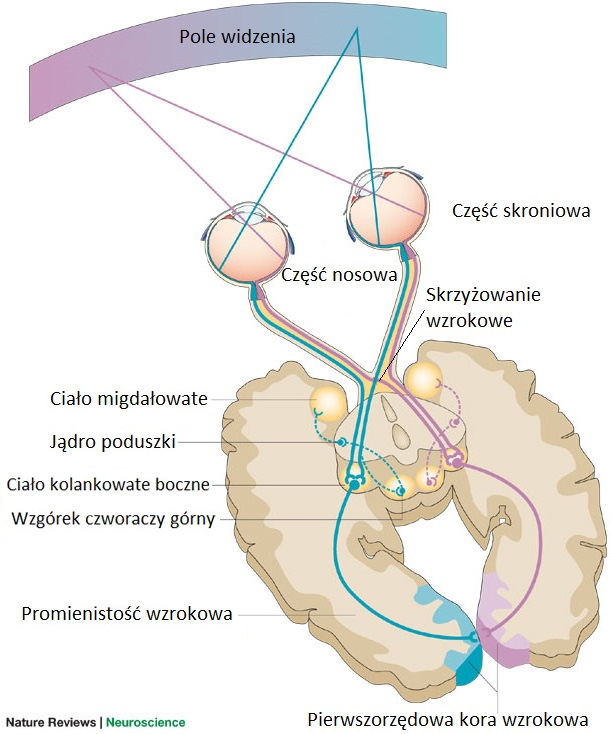
\includegraphics[scale=0.5]{schemat_ukladu.jpg}
		\end{center}
		\caption{Schemat układu wzrokowego \citep{hannula}.}
		\label{rys:sch_u_wz}
	\end{figure}
	\section{Lokalne potencjały polowe}
	Sygnał rejestrowany bezpośrednio z kory i warstw podkorowych nazywany jest elektrokorykogramem. Elektrokortykografia jest metodą inwazyjną i tylko w  wyjątkowych okolicznościach przeprowadza się ją na ludziach. Elektrody umieszczone są tuż obok neuronów -- zbiera się w ten sposób zapis aktywności mózgu z niewielkiego obszaru. Zapis ten zwany jest lokalnymi potencjałami polowymi (ang. \textit{Local Field Potentials}). W odróżnieniu od sygnału z powierzchni głowy, w LFP rejestruje się nie tylko potencjał postsynaptyczny (Rysunek \ref{rys:epsp}), ale także czynnościowy (Rysunek \ref{rys:pot_spoczy}).
	
	Potencjały postsynaptyczne są to potencjały docierające do dendrytu komórki nerwowej. Występują dwa rodzaje:
	\begin{itemize}
		\item potencjały pobudzające EPSP (z ang. \textit{Excitatory Post-Synaptic Potentials})
		\item potencjały hamujące IPSP (z ang. \textit{Inhibitory Post-Synaptic Potentials}) 
	\end{itemize}
	Pierwsze z nich zwiększają szansę na wywołanie potencjału czynnościowego, a drugie tę szansę zmniejszają. Do neuronu dociera równocześnie wiele potencjałów. W chwili, gdy ich suma przekroczy pewną wartość graniczną, neuron zostaje pobudzony. Generuje potencjał czynnościowy, który propaguje się wzdłuż aksonu.
	\begin{figure}[htbp]
		\begin{center}
			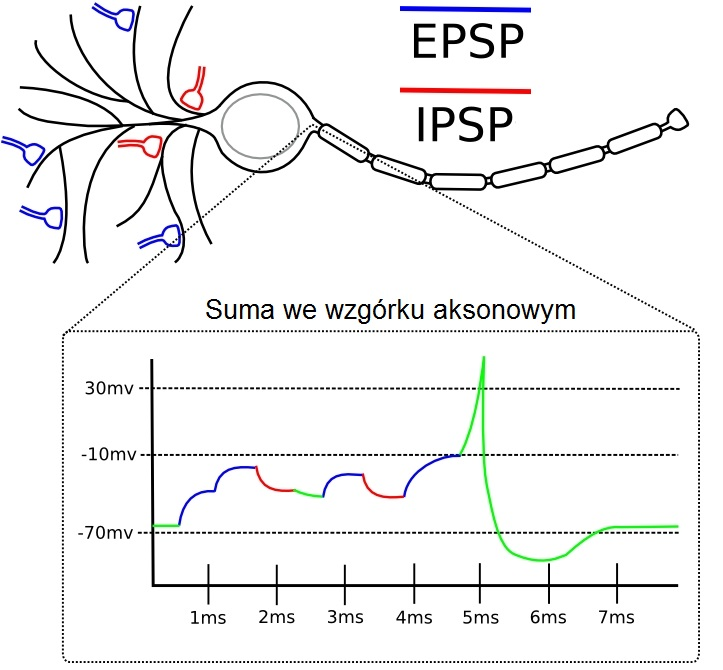
\includegraphics[scale=0.5]{epsp.jpg}
		\end{center}
		\caption{Schemat potencjałów postsynaptycznych \citep{versace}.}
		\label{rys:epsp}
	\end{figure}
	\begin{figure}[htbp]
		\begin{center}
			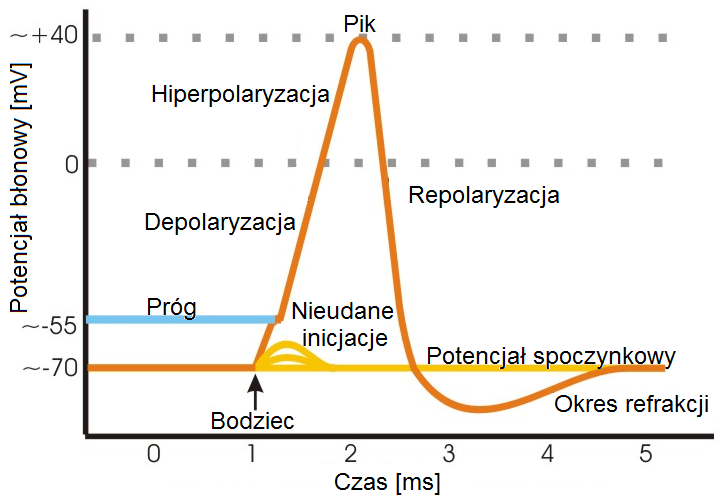
\includegraphics[scale=0.5]{pot_spoczy.png}
		\end{center}
		\caption{Schemat potencjału czynnościowego.}
		\label{rys:pot_spoczy}
	\end{figure}
	\newpage
	\section{Warstwowa budowa struktur}
	Zarówno kora wzrokowa jak i wzgórek czworaczy górny charakteryzują się warstwową budową. Poszczególne warstwy różnią się funkcją oraz połączeniami do innych struktur. 
	Można je rozpoznać za pomocą badania mikroskopowego wybarwionych i wypreparowanych tkanek. Jak pokazały badania, w obrębie pierwszorzędowej kory wzrokowej jak i wzgórka czworaczego górnego na pewnej głębokości obserwuje się odwrócenie polaryzacji na wykresach uśrednionych potencjałów wywołanych \citep{maier2, SC_warstwy}.
	\subsection{Kora wzrokowa}
	Na Rysunku \ref{rys:warstwy} przedstawiono schematyczną strukturę warstwową pierwszorzędowej kory wzrokowej u makaka rezusa.
	\begin{figure}[htbp]
		\begin{center}
			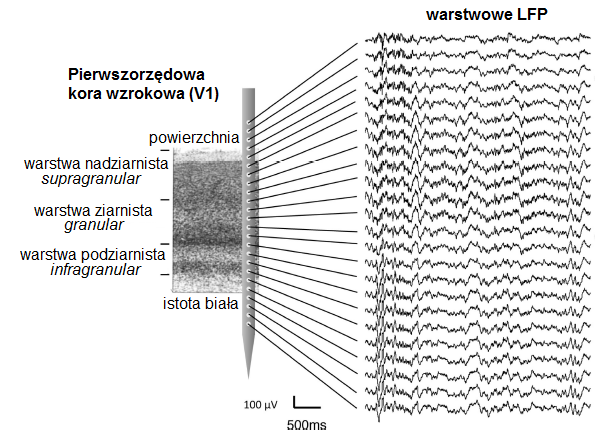
\includegraphics[scale=0.55]{warstwy.png}
		\end{center}
		\caption{Struktura warstwowa pierwszorzędowej kory wzrokowej \citep{kora_warstwy}.}
		\label{rys:warstwy}
	\end{figure}
	\FloatBarrier
	\subsection{Wzgórek czworaczy górny}
	Na Rysunku \ref{rys:SC_warstwy} przedstawiono schematyczną strukturę wzgórka czworaczego górnego u fretki. 
	%\begin{itemize}
	%	\item[SZ] - \textit{stratum zonale}
	%	\item[SGS] - \textit{stratum griseum superficiale}
	%	\item[SO] - \textit{stratum opticum}
	%	\item[SGI] - \textit{stratum griseum intermediale}
	%	\item[ISO] - istota szara okołowodociągowa
	%\end{itemize}
	\begin{figure}[htbp]
		\begin{center}
			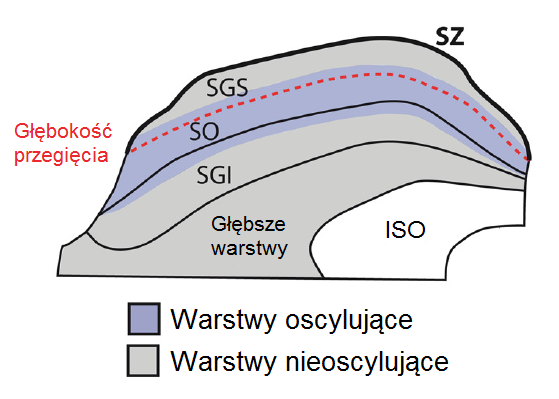
\includegraphics[scale=0.55]{SC_warstwy.png}
		\end{center}
		\caption{Struktura warstwowa wzgórka czworaczego górnego \citep{SC_warstwy}. Skrótami oznaczono: SZ -- \textit{stratum zonale}, SGS -- \textit{stratum griseum superficiale}, SO -- \textit{stratum opticum}, SGI -- \textit{stratum griseum intermediale}, ISO -- istota szara okołowodociągowa.}
		\label{rys:SC_warstwy}
	\end{figure}
	\chapter{Pochodzenie danych doświadczalnych}
	\section{Dane doświadczalne}
	Dane wykorzystane w niniejszej pracy pochodzą z eksperymentów przeprowadzonych w Pracowni Neurobiologii Widzenia Instytutu Biologii Doświadczalnej PAN im. Marcelego Nenckiego w Warszawie. Zostały zebrane przez zespół doświadczalny składający się z dra Andrzeja Foika i mgr inż. Katarzyny Żeber.
	
	W każdym doświadczeniu wykorzystano 2 szczury z gatunku Wistar, po jednym z każdego eksperymentu. Szczury zostały znieczulone dootrzewnowym zastrzykiem z uretanu (2 ml/kg). W mózgu każdego ze zwierząt umieszczono 4 elektrody:
	\begin{itemize}
		\item 1 po stronie ipsilateralnej względem bodźca -- w korze wzrokowej (CxI)
		\item 3 po stronie konralateralnej względem bodźca:
		\begin{itemize}
			\item w korze wzrokowej (CxC)
			\item we wzgórku czworaczym górnym (SC)
			\item w jądrze kolankowatym bocznym (LGN)
		\end{itemize}
	\end{itemize}
	Na każdej elektrodzie znajdowało się od 7 do 16 kontaktów. Oba zestawy danych zawierały różne liczby kanałów. W eksperymencie A do rejestracji aktywności kory wzrokowej wykorzystano 16 kontaktów dla każdej półkuli, a w eksperymencie B -- 8 kontaktów (kontakty były rozmieszczone 2-krotnie rzadziej.) W obu eksperymentach informację ze wzgórka czworaczego zbierano za pomocą 7 kontaktów, a z jądra kolankowatego bocznego -- 8 kontaktów. 
	\section{Procedury eksperymentów}
	Zastosowano dwie różne procedury eksperymentalne opisane poniżej.
	\subsection{Eksperyment A}
	Co 15 minut prezentowano serię bodźców w postaci błyskającego światła, którego źródło umieszczono blisko jednego oka. Jako próbę kontrolną przyjęto pierwszą rejestrację, zakładając, że jest to odpowiedź w stanie nieprzyzwyczajonym do stymulacji. Błyski trwały 2 ms i pojawiały się z różną częstotliwością (przerwy wynosiły od 2 do 2,13 s) 300 razy. Sygnał zbierano co godzinę.
	\subsection{Eksperyment B}
	Czterokrotnie przez pół sekundy stymulowano lewe oko prądem elektrycznym za pomocą niewielkiej elektrody umieszczonej na gałce ocznej. Amplituda prądu wynosiła 2 mA, a częstotliwość 100 Hz. Następnie stymulowano to samo oko bodźcem świetlnym w seriach po 200 błysków (takich jak w eksperymencie A) i co godzinę rejestrowano odpowiedź.
	\FloatBarrier
	Na Rysunku \ref{rys:porownanie_paradygmatow} przedstawiono szkic przebiegów czasowych obu warunków doświadczalnych. 
	\begin{figure}
		%% Created by tikzDevice version 0.7.0 on 2015-06-24 21:37:33
% !TEX encoding = UTF-8 Unicode
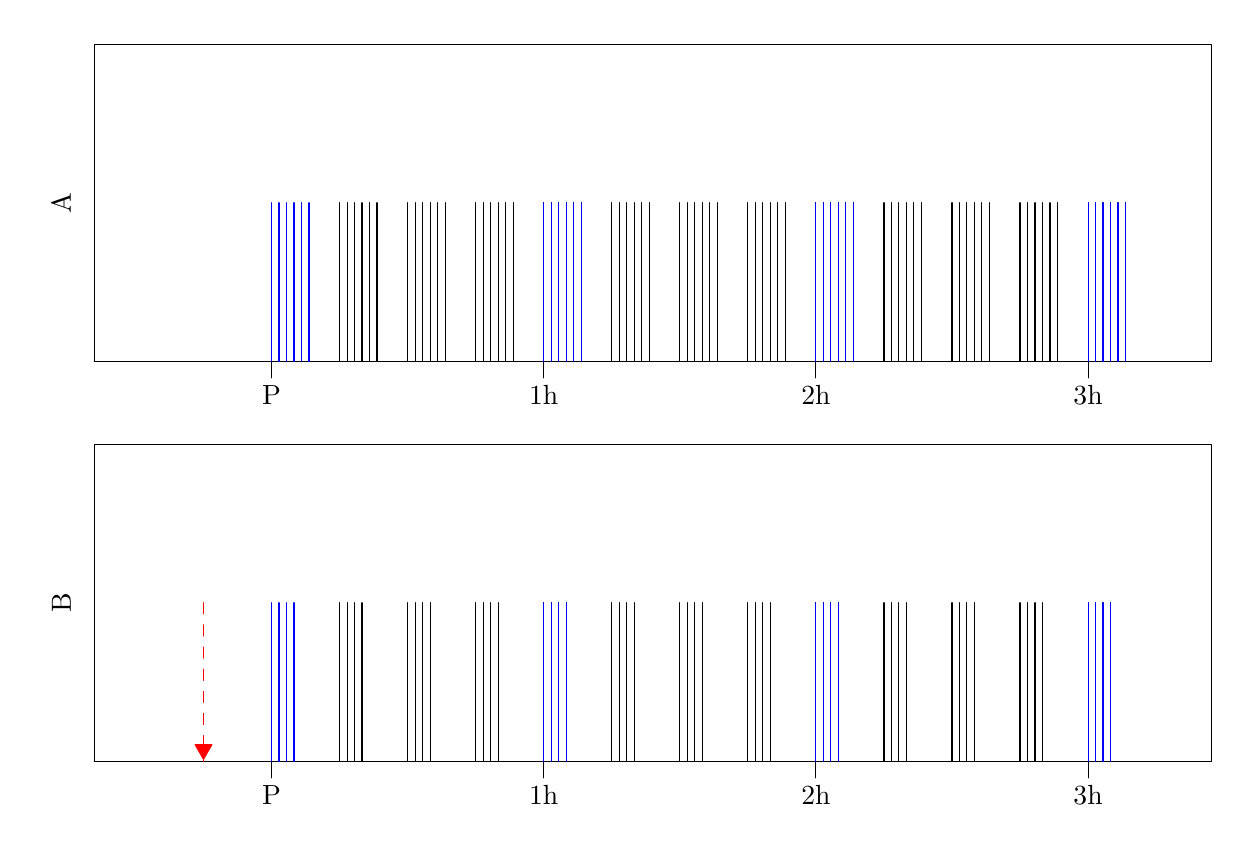
\begin{tikzpicture}[x=1pt,y=1pt]
\definecolor[named]{fillColor}{rgb}{1.00,1.00,1.00}
\path[use as bounding box,fill=fillColor,fill opacity=0.00] (0,0) rectangle (433.62,289.08);
\begin{scope}
\path[clip] (  0.00,  0.00) rectangle (433.62,289.08);
\definecolor[named]{drawColor}{rgb}{0.00,0.00,0.00}

\path[draw=drawColor,line width= 0.4pt,line join=round,line cap=round] ( 24.00,168.54) --
	(427.62,168.54) --
	(427.62,283.08) --
	( 24.00,283.08) --
	( 24.00,168.54);
\end{scope}
\begin{scope}
\path[clip] (  0.00,144.54) rectangle (433.62,289.08);
\definecolor[named]{drawColor}{rgb}{0.00,0.00,0.00}

\node[text=drawColor,rotate= 90.00,anchor=base,inner sep=0pt, outer sep=0pt, scale=  1.00] at ( 15.60,225.81) {A};
\end{scope}
\begin{scope}
\path[clip] (  0.00,  0.00) rectangle (433.62,289.08);
\definecolor[named]{drawColor}{rgb}{0.00,0.00,0.00}

\path[draw=drawColor,line width= 0.4pt,line join=round,line cap=round] ( 88.12,168.54) -- (383.17,168.54);

\path[draw=drawColor,line width= 0.4pt,line join=round,line cap=round] ( 88.12,168.54) -- ( 88.12,162.54);

\path[draw=drawColor,line width= 0.4pt,line join=round,line cap=round] (186.47,168.54) -- (186.47,162.54);

\path[draw=drawColor,line width= 0.4pt,line join=round,line cap=round] (284.82,168.54) -- (284.82,162.54);

\path[draw=drawColor,line width= 0.4pt,line join=round,line cap=round] (383.17,168.54) -- (383.17,162.54);

\node[text=drawColor,anchor=base,inner sep=0pt, outer sep=0pt, scale=  1.00] at ( 88.12,152.94) {P};

\node[text=drawColor,anchor=base,inner sep=0pt, outer sep=0pt, scale=  1.00] at (186.47,152.94) {1h};

\node[text=drawColor,anchor=base,inner sep=0pt, outer sep=0pt, scale=  1.00] at (284.82,152.94) {2h};

\node[text=drawColor,anchor=base,inner sep=0pt, outer sep=0pt, scale=  1.00] at (383.17,152.94) {3h};
\end{scope}
\begin{scope}
\path[clip] ( 24.00,168.54) rectangle (427.62,283.08);
\definecolor[named]{drawColor}{rgb}{0.00,0.00,1.00}

\path[draw=drawColor,line width= 0.4pt,line join=round,line cap=round] ( 88.12, 66.73) -- ( 88.12,225.81);

\path[draw=drawColor,line width= 0.4pt,line join=round,line cap=round] ( 90.83, 66.73) -- ( 90.83,225.81);

\path[draw=drawColor,line width= 0.4pt,line join=round,line cap=round] ( 93.53, 66.73) -- ( 93.53,225.81);

\path[draw=drawColor,line width= 0.4pt,line join=round,line cap=round] ( 96.24, 66.73) -- ( 96.24,225.81);

\path[draw=drawColor,line width= 0.4pt,line join=round,line cap=round] ( 98.94, 66.73) -- ( 98.94,225.81);

\path[draw=drawColor,line width= 0.4pt,line join=round,line cap=round] (101.65, 66.73) -- (101.65,225.81);
\definecolor[named]{drawColor}{rgb}{0.00,0.00,0.00}

\path[draw=drawColor,line width= 0.4pt,line join=round,line cap=round] (112.71, 66.73) -- (112.71,225.81);

\path[draw=drawColor,line width= 0.4pt,line join=round,line cap=round] (115.41, 66.73) -- (115.41,225.81);

\path[draw=drawColor,line width= 0.4pt,line join=round,line cap=round] (118.12, 66.73) -- (118.12,225.81);

\path[draw=drawColor,line width= 0.4pt,line join=round,line cap=round] (120.82, 66.73) -- (120.82,225.81);

\path[draw=drawColor,line width= 0.4pt,line join=round,line cap=round] (123.53, 66.73) -- (123.53,225.81);

\path[draw=drawColor,line width= 0.4pt,line join=round,line cap=round] (126.23, 66.73) -- (126.23,225.81);

\path[draw=drawColor,line width= 0.4pt,line join=round,line cap=round] (137.30, 66.73) -- (137.30,225.81);

\path[draw=drawColor,line width= 0.4pt,line join=round,line cap=round] (140.00, 66.73) -- (140.00,225.81);

\path[draw=drawColor,line width= 0.4pt,line join=round,line cap=round] (142.71, 66.73) -- (142.71,225.81);

\path[draw=drawColor,line width= 0.4pt,line join=round,line cap=round] (145.41, 66.73) -- (145.41,225.81);

\path[draw=drawColor,line width= 0.4pt,line join=round,line cap=round] (148.12, 66.73) -- (148.12,225.81);

\path[draw=drawColor,line width= 0.4pt,line join=round,line cap=round] (150.82, 66.73) -- (150.82,225.81);

\path[draw=drawColor,line width= 0.4pt,line join=round,line cap=round] (161.88, 66.73) -- (161.88,225.81);

\path[draw=drawColor,line width= 0.4pt,line join=round,line cap=round] (164.59, 66.73) -- (164.59,225.81);

\path[draw=drawColor,line width= 0.4pt,line join=round,line cap=round] (167.29, 66.73) -- (167.29,225.81);

\path[draw=drawColor,line width= 0.4pt,line join=round,line cap=round] (170.00, 66.73) -- (170.00,225.81);

\path[draw=drawColor,line width= 0.4pt,line join=round,line cap=round] (172.70, 66.73) -- (172.70,225.81);

\path[draw=drawColor,line width= 0.4pt,line join=round,line cap=round] (175.41, 66.73) -- (175.41,225.81);

\path[draw=drawColor,line width= 0.4pt,line join=round,line cap=round] (186.47, 66.73) -- (186.47,225.81);

\path[draw=drawColor,line width= 0.4pt,line join=round,line cap=round] (189.18, 66.73) -- (189.18,225.81);

\path[draw=drawColor,line width= 0.4pt,line join=round,line cap=round] (191.88, 66.73) -- (191.88,225.81);

\path[draw=drawColor,line width= 0.4pt,line join=round,line cap=round] (194.58, 66.73) -- (194.58,225.81);

\path[draw=drawColor,line width= 0.4pt,line join=round,line cap=round] (197.29, 66.73) -- (197.29,225.81);

\path[draw=drawColor,line width= 0.4pt,line join=round,line cap=round] (199.99, 66.73) -- (199.99,225.81);
\definecolor[named]{drawColor}{rgb}{0.00,0.00,1.00}

\path[draw=drawColor,line width= 0.4pt,line join=round,line cap=round] (186.47, 66.73) -- (186.47,225.81);

\path[draw=drawColor,line width= 0.4pt,line join=round,line cap=round] (189.18, 66.73) -- (189.18,225.81);

\path[draw=drawColor,line width= 0.4pt,line join=round,line cap=round] (191.88, 66.73) -- (191.88,225.81);

\path[draw=drawColor,line width= 0.4pt,line join=round,line cap=round] (194.58, 66.73) -- (194.58,225.81);

\path[draw=drawColor,line width= 0.4pt,line join=round,line cap=round] (197.29, 66.73) -- (197.29,225.81);

\path[draw=drawColor,line width= 0.4pt,line join=round,line cap=round] (199.99, 66.73) -- (199.99,225.81);
\definecolor[named]{drawColor}{rgb}{0.00,0.00,0.00}

\path[draw=drawColor,line width= 0.4pt,line join=round,line cap=round] (211.06, 66.73) -- (211.06,225.81);

\path[draw=drawColor,line width= 0.4pt,line join=round,line cap=round] (213.76, 66.73) -- (213.76,225.81);

\path[draw=drawColor,line width= 0.4pt,line join=round,line cap=round] (216.47, 66.73) -- (216.47,225.81);

\path[draw=drawColor,line width= 0.4pt,line join=round,line cap=round] (219.17, 66.73) -- (219.17,225.81);

\path[draw=drawColor,line width= 0.4pt,line join=round,line cap=round] (221.88, 66.73) -- (221.88,225.81);

\path[draw=drawColor,line width= 0.4pt,line join=round,line cap=round] (224.58, 66.73) -- (224.58,225.81);

\path[draw=drawColor,line width= 0.4pt,line join=round,line cap=round] (235.64, 66.73) -- (235.64,225.81);

\path[draw=drawColor,line width= 0.4pt,line join=round,line cap=round] (238.35, 66.73) -- (238.35,225.81);

\path[draw=drawColor,line width= 0.4pt,line join=round,line cap=round] (241.05, 66.73) -- (241.05,225.81);

\path[draw=drawColor,line width= 0.4pt,line join=round,line cap=round] (243.76, 66.73) -- (243.76,225.81);

\path[draw=drawColor,line width= 0.4pt,line join=round,line cap=round] (246.46, 66.73) -- (246.46,225.81);

\path[draw=drawColor,line width= 0.4pt,line join=round,line cap=round] (249.17, 66.73) -- (249.17,225.81);

\path[draw=drawColor,line width= 0.4pt,line join=round,line cap=round] (260.23, 66.73) -- (260.23,225.81);

\path[draw=drawColor,line width= 0.4pt,line join=round,line cap=round] (262.94, 66.73) -- (262.94,225.81);

\path[draw=drawColor,line width= 0.4pt,line join=round,line cap=round] (265.64, 66.73) -- (265.64,225.81);

\path[draw=drawColor,line width= 0.4pt,line join=round,line cap=round] (268.35, 66.73) -- (268.35,225.81);

\path[draw=drawColor,line width= 0.4pt,line join=round,line cap=round] (271.05, 66.73) -- (271.05,225.81);

\path[draw=drawColor,line width= 0.4pt,line join=round,line cap=round] (273.75, 66.73) -- (273.75,225.81);

\path[draw=drawColor,line width= 0.4pt,line join=round,line cap=round] (284.82, 66.73) -- (284.82,225.81);

\path[draw=drawColor,line width= 0.4pt,line join=round,line cap=round] (287.52, 66.73) -- (287.52,225.81);

\path[draw=drawColor,line width= 0.4pt,line join=round,line cap=round] (290.23, 66.73) -- (290.23,225.81);

\path[draw=drawColor,line width= 0.4pt,line join=round,line cap=round] (292.93, 66.73) -- (292.93,225.81);

\path[draw=drawColor,line width= 0.4pt,line join=round,line cap=round] (295.64, 66.73) -- (295.64,225.81);

\path[draw=drawColor,line width= 0.4pt,line join=round,line cap=round] (298.34, 66.73) -- (298.34,225.81);
\definecolor[named]{drawColor}{rgb}{0.00,0.00,1.00}

\path[draw=drawColor,line width= 0.4pt,line join=round,line cap=round] (284.82, 66.73) -- (284.82,225.81);

\path[draw=drawColor,line width= 0.4pt,line join=round,line cap=round] (287.52, 66.73) -- (287.52,225.81);

\path[draw=drawColor,line width= 0.4pt,line join=round,line cap=round] (290.23, 66.73) -- (290.23,225.81);

\path[draw=drawColor,line width= 0.4pt,line join=round,line cap=round] (292.93, 66.73) -- (292.93,225.81);

\path[draw=drawColor,line width= 0.4pt,line join=round,line cap=round] (295.64, 66.73) -- (295.64,225.81);

\path[draw=drawColor,line width= 0.4pt,line join=round,line cap=round] (298.34, 66.73) -- (298.34,225.81);
\definecolor[named]{drawColor}{rgb}{0.00,0.00,0.00}

\path[draw=drawColor,line width= 0.4pt,line join=round,line cap=round] (309.41, 66.73) -- (309.41,225.81);

\path[draw=drawColor,line width= 0.4pt,line join=round,line cap=round] (312.11, 66.73) -- (312.11,225.81);

\path[draw=drawColor,line width= 0.4pt,line join=round,line cap=round] (314.81, 66.73) -- (314.81,225.81);

\path[draw=drawColor,line width= 0.4pt,line join=round,line cap=round] (317.52, 66.73) -- (317.52,225.81);

\path[draw=drawColor,line width= 0.4pt,line join=round,line cap=round] (320.22, 66.73) -- (320.22,225.81);

\path[draw=drawColor,line width= 0.4pt,line join=round,line cap=round] (322.93, 66.73) -- (322.93,225.81);

\path[draw=drawColor,line width= 0.4pt,line join=round,line cap=round] (333.99, 66.73) -- (333.99,225.81);

\path[draw=drawColor,line width= 0.4pt,line join=round,line cap=round] (336.70, 66.73) -- (336.70,225.81);

\path[draw=drawColor,line width= 0.4pt,line join=round,line cap=round] (339.40, 66.73) -- (339.40,225.81);

\path[draw=drawColor,line width= 0.4pt,line join=round,line cap=round] (342.11, 66.73) -- (342.11,225.81);

\path[draw=drawColor,line width= 0.4pt,line join=round,line cap=round] (344.81, 66.73) -- (344.81,225.81);

\path[draw=drawColor,line width= 0.4pt,line join=round,line cap=round] (347.52, 66.73) -- (347.52,225.81);

\path[draw=drawColor,line width= 0.4pt,line join=round,line cap=round] (358.58, 66.73) -- (358.58,225.81);

\path[draw=drawColor,line width= 0.4pt,line join=round,line cap=round] (361.28, 66.73) -- (361.28,225.81);

\path[draw=drawColor,line width= 0.4pt,line join=round,line cap=round] (363.99, 66.73) -- (363.99,225.81);

\path[draw=drawColor,line width= 0.4pt,line join=round,line cap=round] (366.69, 66.73) -- (366.69,225.81);

\path[draw=drawColor,line width= 0.4pt,line join=round,line cap=round] (369.40, 66.73) -- (369.40,225.81);

\path[draw=drawColor,line width= 0.4pt,line join=round,line cap=round] (372.10, 66.73) -- (372.10,225.81);

\path[draw=drawColor,line width= 0.4pt,line join=round,line cap=round] (383.17, 66.73) -- (383.17,225.81);

\path[draw=drawColor,line width= 0.4pt,line join=round,line cap=round] (385.87, 66.73) -- (385.87,225.81);

\path[draw=drawColor,line width= 0.4pt,line join=round,line cap=round] (388.58, 66.73) -- (388.58,225.81);

\path[draw=drawColor,line width= 0.4pt,line join=round,line cap=round] (391.28, 66.73) -- (391.28,225.81);

\path[draw=drawColor,line width= 0.4pt,line join=round,line cap=round] (393.99, 66.73) -- (393.99,225.81);

\path[draw=drawColor,line width= 0.4pt,line join=round,line cap=round] (396.69, 66.73) -- (396.69,225.81);
\definecolor[named]{drawColor}{rgb}{0.00,0.00,1.00}

\path[draw=drawColor,line width= 0.4pt,line join=round,line cap=round] (383.17, 66.73) -- (383.17,225.81);

\path[draw=drawColor,line width= 0.4pt,line join=round,line cap=round] (385.87, 66.73) -- (385.87,225.81);

\path[draw=drawColor,line width= 0.4pt,line join=round,line cap=round] (388.58, 66.73) -- (388.58,225.81);

\path[draw=drawColor,line width= 0.4pt,line join=round,line cap=round] (391.28, 66.73) -- (391.28,225.81);

\path[draw=drawColor,line width= 0.4pt,line join=round,line cap=round] (393.99, 66.73) -- (393.99,225.81);

\path[draw=drawColor,line width= 0.4pt,line join=round,line cap=round] (396.69, 66.73) -- (396.69,225.81);
\end{scope}
\begin{scope}
\path[clip] (  0.00,  0.00) rectangle (433.62,289.08);
\definecolor[named]{drawColor}{rgb}{0.00,0.00,0.00}

\path[draw=drawColor,line width= 0.4pt,line join=round,line cap=round] ( 24.00, 24.00) --
	(427.62, 24.00) --
	(427.62,138.54) --
	( 24.00,138.54) --
	( 24.00, 24.00);
\end{scope}
\begin{scope}
\path[clip] (  0.00,  0.00) rectangle (433.62,144.54);
\definecolor[named]{drawColor}{rgb}{0.00,0.00,0.00}

\node[text=drawColor,rotate= 90.00,anchor=base,inner sep=0pt, outer sep=0pt, scale=  1.00] at ( 15.60, 81.27) {B};
\end{scope}
\begin{scope}
\path[clip] (  0.00,  0.00) rectangle (433.62,289.08);
\definecolor[named]{drawColor}{rgb}{0.00,0.00,0.00}

\path[draw=drawColor,line width= 0.4pt,line join=round,line cap=round] ( 88.12, 24.00) -- (383.17, 24.00);

\path[draw=drawColor,line width= 0.4pt,line join=round,line cap=round] ( 88.12, 24.00) -- ( 88.12, 18.00);

\path[draw=drawColor,line width= 0.4pt,line join=round,line cap=round] (186.47, 24.00) -- (186.47, 18.00);

\path[draw=drawColor,line width= 0.4pt,line join=round,line cap=round] (284.82, 24.00) -- (284.82, 18.00);

\path[draw=drawColor,line width= 0.4pt,line join=round,line cap=round] (383.17, 24.00) -- (383.17, 18.00);

\node[text=drawColor,anchor=base,inner sep=0pt, outer sep=0pt, scale=  1.00] at ( 88.12,  8.40) {P};

\node[text=drawColor,anchor=base,inner sep=0pt, outer sep=0pt, scale=  1.00] at (186.47,  8.40) {1h};

\node[text=drawColor,anchor=base,inner sep=0pt, outer sep=0pt, scale=  1.00] at (284.82,  8.40) {2h};

\node[text=drawColor,anchor=base,inner sep=0pt, outer sep=0pt, scale=  1.00] at (383.17,  8.40) {3h};
\end{scope}
\begin{scope}
\path[clip] ( 24.00, 24.00) rectangle (427.62,138.54);
\definecolor[named]{drawColor}{rgb}{0.00,0.00,1.00}

\path[draw=drawColor,line width= 0.4pt,line join=round,line cap=round] ( 88.12,  0.00) -- ( 88.12, 81.27);

\path[draw=drawColor,line width= 0.4pt,line join=round,line cap=round] ( 90.83,  0.00) -- ( 90.83, 81.27);

\path[draw=drawColor,line width= 0.4pt,line join=round,line cap=round] ( 93.53,  0.00) -- ( 93.53, 81.27);

\path[draw=drawColor,line width= 0.4pt,line join=round,line cap=round] ( 96.24,  0.00) -- ( 96.24, 81.27);
\definecolor[named]{drawColor}{rgb}{0.00,0.00,0.00}

\path[draw=drawColor,line width= 0.4pt,line join=round,line cap=round] (112.71,  0.00) -- (112.71, 81.27);

\path[draw=drawColor,line width= 0.4pt,line join=round,line cap=round] (115.41,  0.00) -- (115.41, 81.27);

\path[draw=drawColor,line width= 0.4pt,line join=round,line cap=round] (118.12,  0.00) -- (118.12, 81.27);

\path[draw=drawColor,line width= 0.4pt,line join=round,line cap=round] (120.82,  0.00) -- (120.82, 81.27);

\path[draw=drawColor,line width= 0.4pt,line join=round,line cap=round] (137.30,  0.00) -- (137.30, 81.27);

\path[draw=drawColor,line width= 0.4pt,line join=round,line cap=round] (140.00,  0.00) -- (140.00, 81.27);

\path[draw=drawColor,line width= 0.4pt,line join=round,line cap=round] (142.71,  0.00) -- (142.71, 81.27);

\path[draw=drawColor,line width= 0.4pt,line join=round,line cap=round] (145.41,  0.00) -- (145.41, 81.27);

\path[draw=drawColor,line width= 0.4pt,line join=round,line cap=round] (161.88,  0.00) -- (161.88, 81.27);

\path[draw=drawColor,line width= 0.4pt,line join=round,line cap=round] (164.59,  0.00) -- (164.59, 81.27);

\path[draw=drawColor,line width= 0.4pt,line join=round,line cap=round] (167.29,  0.00) -- (167.29, 81.27);

\path[draw=drawColor,line width= 0.4pt,line join=round,line cap=round] (170.00,  0.00) -- (170.00, 81.27);

\path[draw=drawColor,line width= 0.4pt,line join=round,line cap=round] (186.47,  0.00) -- (186.47, 81.27);

\path[draw=drawColor,line width= 0.4pt,line join=round,line cap=round] (189.18,  0.00) -- (189.18, 81.27);

\path[draw=drawColor,line width= 0.4pt,line join=round,line cap=round] (191.88,  0.00) -- (191.88, 81.27);

\path[draw=drawColor,line width= 0.4pt,line join=round,line cap=round] (194.58,  0.00) -- (194.58, 81.27);
\definecolor[named]{drawColor}{rgb}{0.00,0.00,1.00}

\path[draw=drawColor,line width= 0.4pt,line join=round,line cap=round] (186.47,  0.00) -- (186.47, 81.27);

\path[draw=drawColor,line width= 0.4pt,line join=round,line cap=round] (189.18,  0.00) -- (189.18, 81.27);

\path[draw=drawColor,line width= 0.4pt,line join=round,line cap=round] (191.88,  0.00) -- (191.88, 81.27);

\path[draw=drawColor,line width= 0.4pt,line join=round,line cap=round] (194.58,  0.00) -- (194.58, 81.27);
\definecolor[named]{drawColor}{rgb}{0.00,0.00,0.00}

\path[draw=drawColor,line width= 0.4pt,line join=round,line cap=round] (211.06,  0.00) -- (211.06, 81.27);

\path[draw=drawColor,line width= 0.4pt,line join=round,line cap=round] (213.76,  0.00) -- (213.76, 81.27);

\path[draw=drawColor,line width= 0.4pt,line join=round,line cap=round] (216.47,  0.00) -- (216.47, 81.27);

\path[draw=drawColor,line width= 0.4pt,line join=round,line cap=round] (219.17,  0.00) -- (219.17, 81.27);

\path[draw=drawColor,line width= 0.4pt,line join=round,line cap=round] (235.64,  0.00) -- (235.64, 81.27);

\path[draw=drawColor,line width= 0.4pt,line join=round,line cap=round] (238.35,  0.00) -- (238.35, 81.27);

\path[draw=drawColor,line width= 0.4pt,line join=round,line cap=round] (241.05,  0.00) -- (241.05, 81.27);

\path[draw=drawColor,line width= 0.4pt,line join=round,line cap=round] (243.76,  0.00) -- (243.76, 81.27);

\path[draw=drawColor,line width= 0.4pt,line join=round,line cap=round] (260.23,  0.00) -- (260.23, 81.27);

\path[draw=drawColor,line width= 0.4pt,line join=round,line cap=round] (262.94,  0.00) -- (262.94, 81.27);

\path[draw=drawColor,line width= 0.4pt,line join=round,line cap=round] (265.64,  0.00) -- (265.64, 81.27);

\path[draw=drawColor,line width= 0.4pt,line join=round,line cap=round] (268.35,  0.00) -- (268.35, 81.27);

\path[draw=drawColor,line width= 0.4pt,line join=round,line cap=round] (284.82,  0.00) -- (284.82, 81.27);

\path[draw=drawColor,line width= 0.4pt,line join=round,line cap=round] (287.52,  0.00) -- (287.52, 81.27);

\path[draw=drawColor,line width= 0.4pt,line join=round,line cap=round] (290.23,  0.00) -- (290.23, 81.27);

\path[draw=drawColor,line width= 0.4pt,line join=round,line cap=round] (292.93,  0.00) -- (292.93, 81.27);
\definecolor[named]{drawColor}{rgb}{0.00,0.00,1.00}

\path[draw=drawColor,line width= 0.4pt,line join=round,line cap=round] (284.82,  0.00) -- (284.82, 81.27);

\path[draw=drawColor,line width= 0.4pt,line join=round,line cap=round] (287.52,  0.00) -- (287.52, 81.27);

\path[draw=drawColor,line width= 0.4pt,line join=round,line cap=round] (290.23,  0.00) -- (290.23, 81.27);

\path[draw=drawColor,line width= 0.4pt,line join=round,line cap=round] (292.93,  0.00) -- (292.93, 81.27);
\definecolor[named]{drawColor}{rgb}{0.00,0.00,0.00}

\path[draw=drawColor,line width= 0.4pt,line join=round,line cap=round] (309.41,  0.00) -- (309.41, 81.27);

\path[draw=drawColor,line width= 0.4pt,line join=round,line cap=round] (312.11,  0.00) -- (312.11, 81.27);

\path[draw=drawColor,line width= 0.4pt,line join=round,line cap=round] (314.81,  0.00) -- (314.81, 81.27);

\path[draw=drawColor,line width= 0.4pt,line join=round,line cap=round] (317.52,  0.00) -- (317.52, 81.27);

\path[draw=drawColor,line width= 0.4pt,line join=round,line cap=round] (333.99,  0.00) -- (333.99, 81.27);

\path[draw=drawColor,line width= 0.4pt,line join=round,line cap=round] (336.70,  0.00) -- (336.70, 81.27);

\path[draw=drawColor,line width= 0.4pt,line join=round,line cap=round] (339.40,  0.00) -- (339.40, 81.27);

\path[draw=drawColor,line width= 0.4pt,line join=round,line cap=round] (342.11,  0.00) -- (342.11, 81.27);

\path[draw=drawColor,line width= 0.4pt,line join=round,line cap=round] (358.58,  0.00) -- (358.58, 81.27);

\path[draw=drawColor,line width= 0.4pt,line join=round,line cap=round] (361.28,  0.00) -- (361.28, 81.27);

\path[draw=drawColor,line width= 0.4pt,line join=round,line cap=round] (363.99,  0.00) -- (363.99, 81.27);

\path[draw=drawColor,line width= 0.4pt,line join=round,line cap=round] (366.69,  0.00) -- (366.69, 81.27);

\path[draw=drawColor,line width= 0.4pt,line join=round,line cap=round] (383.17,  0.00) -- (383.17, 81.27);

\path[draw=drawColor,line width= 0.4pt,line join=round,line cap=round] (385.87,  0.00) -- (385.87, 81.27);

\path[draw=drawColor,line width= 0.4pt,line join=round,line cap=round] (388.58,  0.00) -- (388.58, 81.27);

\path[draw=drawColor,line width= 0.4pt,line join=round,line cap=round] (391.28,  0.00) -- (391.28, 81.27);
\definecolor[named]{drawColor}{rgb}{0.00,0.00,1.00}

\path[draw=drawColor,line width= 0.4pt,line join=round,line cap=round] (383.17,  0.00) -- (383.17, 81.27);

\path[draw=drawColor,line width= 0.4pt,line join=round,line cap=round] (385.87,  0.00) -- (385.87, 81.27);

\path[draw=drawColor,line width= 0.4pt,line join=round,line cap=round] (388.58,  0.00) -- (388.58, 81.27);

\path[draw=drawColor,line width= 0.4pt,line join=round,line cap=round] (391.28,  0.00) -- (391.28, 81.27);
\definecolor[named]{drawColor}{rgb}{1.00,0.00,0.00}

\path[draw=drawColor,line width= 0.4pt,dash pattern=on 4pt off 4pt ,line join=round,line cap=round] ( 63.54, 81.27) -- ( 63.54,  0.00);
\definecolor[named]{fillColor}{rgb}{1.00,0.00,0.00}

\path[draw=drawColor,line width= 0.4pt,line join=round,line cap=round,fill=fillColor] ( 63.54, 24.74) --
	( 66.57, 29.99) --
	( 60.51, 29.99) --
	cycle;
\end{scope}
\end{tikzpicture}

		\begin{center}
			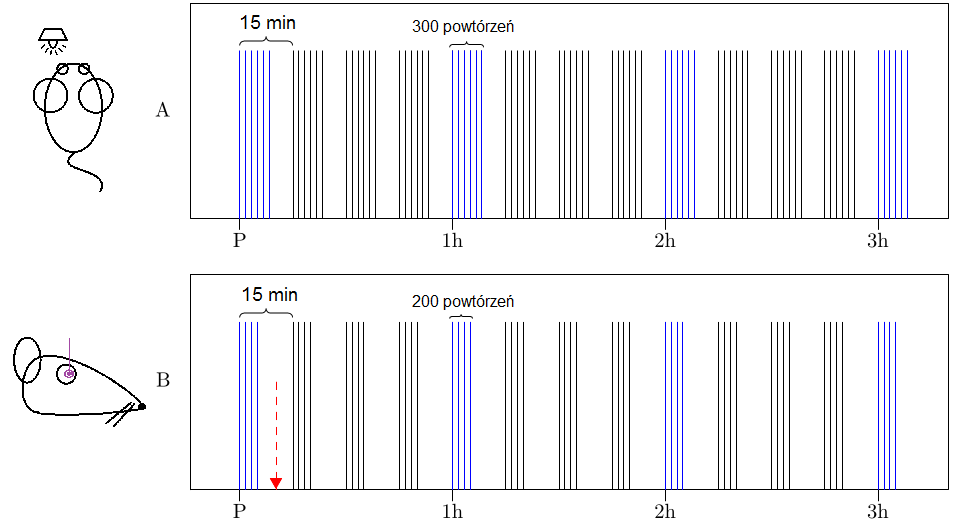
\includegraphics[width=\columnwidth]{przebieg.png}
		\end{center}
		\caption{Przebiegi czasowe obu warunków doświadczalnych. Wykres A odnosi się do eksperymentu A, a wykres B -- do eksperymentu B. Pionowe kreski oznaczają stymulację bodźcem świetlnym (w eksperymencie A było 300 powtórzeń, a w eksperymencie B -- 200). Na niebiesko zaznaczono bodźce, na które odpowiedzi badano, a na czarno -- pozostałe. Czerwona strzałka oznacza moment wystąpienia stymulacji elektrycznej.}
		\label{rys:porownanie_paradygmatow}
	\end{figure}
	\FloatBarrier
	\section{Przygotowanie danych do analizy}
	Sygnał został zarejestrowany z częstotliwością 20 kHz, odfiltrowany pasmowo-przepustowo w przedziale 0,3 - 10 kHz oraz wzmocniony 500-krotnie przy użyciu wzmacniacza prądu zmiennego firmy A-M Systems\textsuperscript{TM} (\texttt{https://www.a-msystems.com/}).
	
	W tej pracy uznano, że tak wysoka częstość próbkowania nie jest potrzebna do dalszej analizy, dlatego zdecydowano się zredukować ją do częstości 250 Hz. W tym celu trzykrotnie na przemian filtrowano sygnał dolnoprzepustowym filtrem Butterwortha II rzędu (częstości odcięcia: 2,5 kHz i 500 Hz) oraz I rzędu (częstość odcięcia: 100 Hz) i decymowano (ang. \textit{downsampling}). Kolejnym krokiem było odfiltrowanie artefaktów pochodzących od napięcia sieciowego (pasmowo-zaporowy filtr Butterwortha I rzędu w przedziale 49,5-50,5 Hz) i usunięcie niskich częstości (górnoprzepustowy filtr Butterwortha I rzędu o częstości odcięcia 1 Hz). Następnie każdą próbkę znormalizowano poprzez odjęcie średniej z całego zapisu dla danego kanału i podzielenie przez odchylenie standardowe.
	
	Filtry Butterwortha zostały wybrane ze względu na to, że tylko w niewielkim stopniu zniekształcają sygnał, ponieważ dają gładką i monotoniczną funkcję odpowiedzi skokowej. Odbywa się to jednak kosztem niskiej skuteczności filtracji. Filtrowano za pomocą funkcji \texttt{filtfilt}, ponieważ nie zmienia fazy sygnału wejściowego.
	
	Tak przygotowanie dane pocięto na odcinki od -0,2 s do 1 s (gdzie 0 było momentem wystąpienia bodźca) i uśredniono po realizacjach.
	
	Do dalszej analizy wybrano po 4 kanały z kory wzrokowej (zarówno kontra- i ispilateralnej względem bodźca) i wzgórka czworaczego oraz jeden kanał z ciała kolankowatego bocznego. Zmniejszenie liczby kanałów było niezbędne z dwóch powodów:
	\begin{itemize}
		\item część kontaktów na elektrodach nie działała poprawnie -- rejestrował się szum, a nie właściwy sygnał
		\item kanały warstw leżących jedna nad drugą były bardzo podobne
	\end{itemize}
	Wyboru dokonano na podstawie analizy uśrednionych potencjałów, patrz Sekcja \ref{sec:zast_pot}.
	\chapter{Metodologia}
	\section{Uśrednianie potencjałów wywołanych}
	\subsection{Opis metody}
	VEP (z ang. \textit{Visual Evoked Potential}) jest szczególnym przypadkiem potencjałów wywołanych stanu ustalonego, gdzie stymulacja odbywa się za pomocą fali świetlnej. W założeniu spontaniczna aktywność ECoG jest procesem stochastycznym (niezależnym, stacjonarnym szumem o średniej zero), a odpowiedź mózgu na każdy z kolejnych bodźców jest niezmienna. Wtedy sygnał mierzony w $i$-tej realizacji możemy wyrazić jako:
	\begin{equation}
		x_i(t) = s(t) + n_i(t),
	\end{equation}
	gdzie $s(t)$ jest rzeczywistym sygnałem, a $n_i(t)$ -- składową szumu. Po uśrednieniu~$N$ realizacji otrzymuje się:
	\begin{equation}
		\bar{x}(t) = \frac{1}{N} \sum_{i=1}^{N} x_i(t) = s(t) + \frac{1}{N}\sum_{i=1}^{N} n_i(t).
	\end{equation}
	Dla szumu o średniej zero, wartość oczekiwana wynosi:
	\begin{equation}
		E\left[ \frac{1}{N}\sum_{i=1}^{N} n_i(t)\right] = 0, 
	\end{equation}
	z czego wynika, że dla uśrednionego sygnału $E\left[ \bar{x}(t) \right] = s(t).$
	
	Na Rysunku \ref{rys:gabor} przedstawiono kolejno:
	\begin{itemize}
		\item funkcję Gabora przed dodaniem szumu
		\item funkcję Gabora z nałożonym szumem
		\item sygnał uśredniony.
	\end{itemize}
	Widać, że na ostatnim wykresie udało się odzyskać pierwotny kształt.
	\begin{figure}[h]
		\begin{center}
			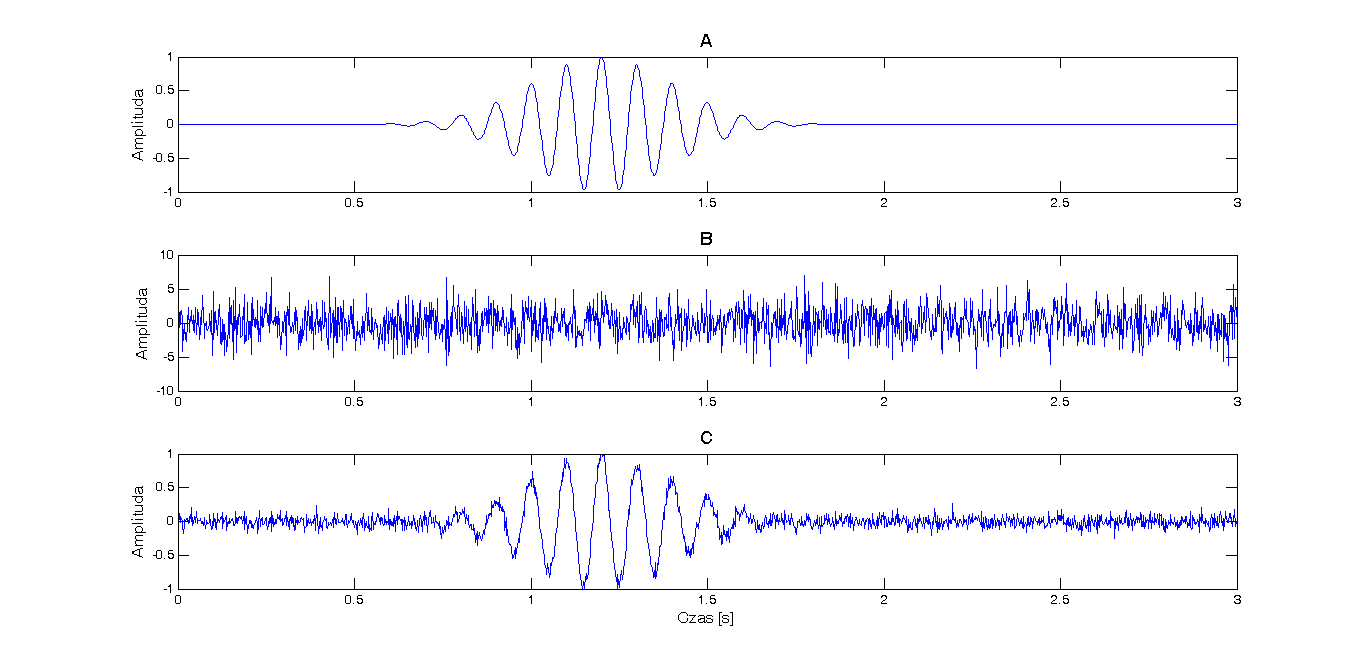
\includegraphics[scale = 0.7]{gabor.png}
		\end{center}
		\caption{Na wykresie A narysowano funkcję Gabora o częstotliwości 10 Hz, odchyleniu standardowym $\sigma_g$~=~0.2 i amplitudzie $A$~=~1. Wykres B przedstawia tę samą funkcję co wykres A po dodaniu 30 składowych szumowych z rozkładu normalnego o średniej $m_{sz}$ = 0 i odchyleniu standardowym $\sigma_{sz}$ = 0.4. Wykres C to 1000 uśrednionych sygnałów z wykresu~B.}
		\label{rys:gabor}
	\end{figure}
	\subsection{Zastosowanie metody}\label{sec:zast_pot}
	Dane z każdego zestawu danych uśredniono po realizacjach i oddzielenie analizowano kanały odpowiadające każdej strukturze mózgu. W pierwszej kolejności odrzucono kanały, w których nie zaobserwowano potencjału wywołanego. Następnie szukano ,,przegięcia'', czyli odwrócenia potencjału w okolicy odpowiedzi na bodziec (czas 0-0,1 s). Jeśli to było możliwe, wybierano kanały bez artefaktu w momencie wystąpienia bodźca (Rysunek \ref{rys:16_kanalow}).
	\subsection{Statystyka}\label{statystyka}
	Żeby sprawdzić, czy wzrost amplitudy potencjału wywołanego między kontrolą a odpowiedzią na bodziec po każdej kolejnej godzinie treningu jest istotny statystycznie, zastosowano metodę bootstrapu. Spośród fragmentów [0; 0,1] s dla wszystkich czasów treningu, dwukrotnie losowano 1000 razy z powtórzeniami po 300 lub 200 fragmentów (odpowiednio dla eksperymentu A i B). Wylosowane fragmenty sygnałów uśredniano po realizacjach uzyskując dwa średnie potencjały bootstrapowe. Dla wyliczonych potencjałów liczono amplitudę \emph{peak-to-peak} i odejmowano uzyskując 1000-elementowy rozkład różnic. Następnie liczono różnicę dla każdej godziny treningu względem kontroli i porównywano z wartościami z bootstrapu. Za próg istotności statystycznej przyjęto $\alpha$ = 0,05. Jednakże ze względu na problem wielokrotnych porównań, zastosowano poprawkę Bonferroniego. Dla każdej struktury mózgowej danego szczura testowano 12 hipotez. Zatem faktyczny próg wynosił $\frac{0,05}{12}=0,0041(6)$.
	\begin{figure}[h]
		\begin{center}
			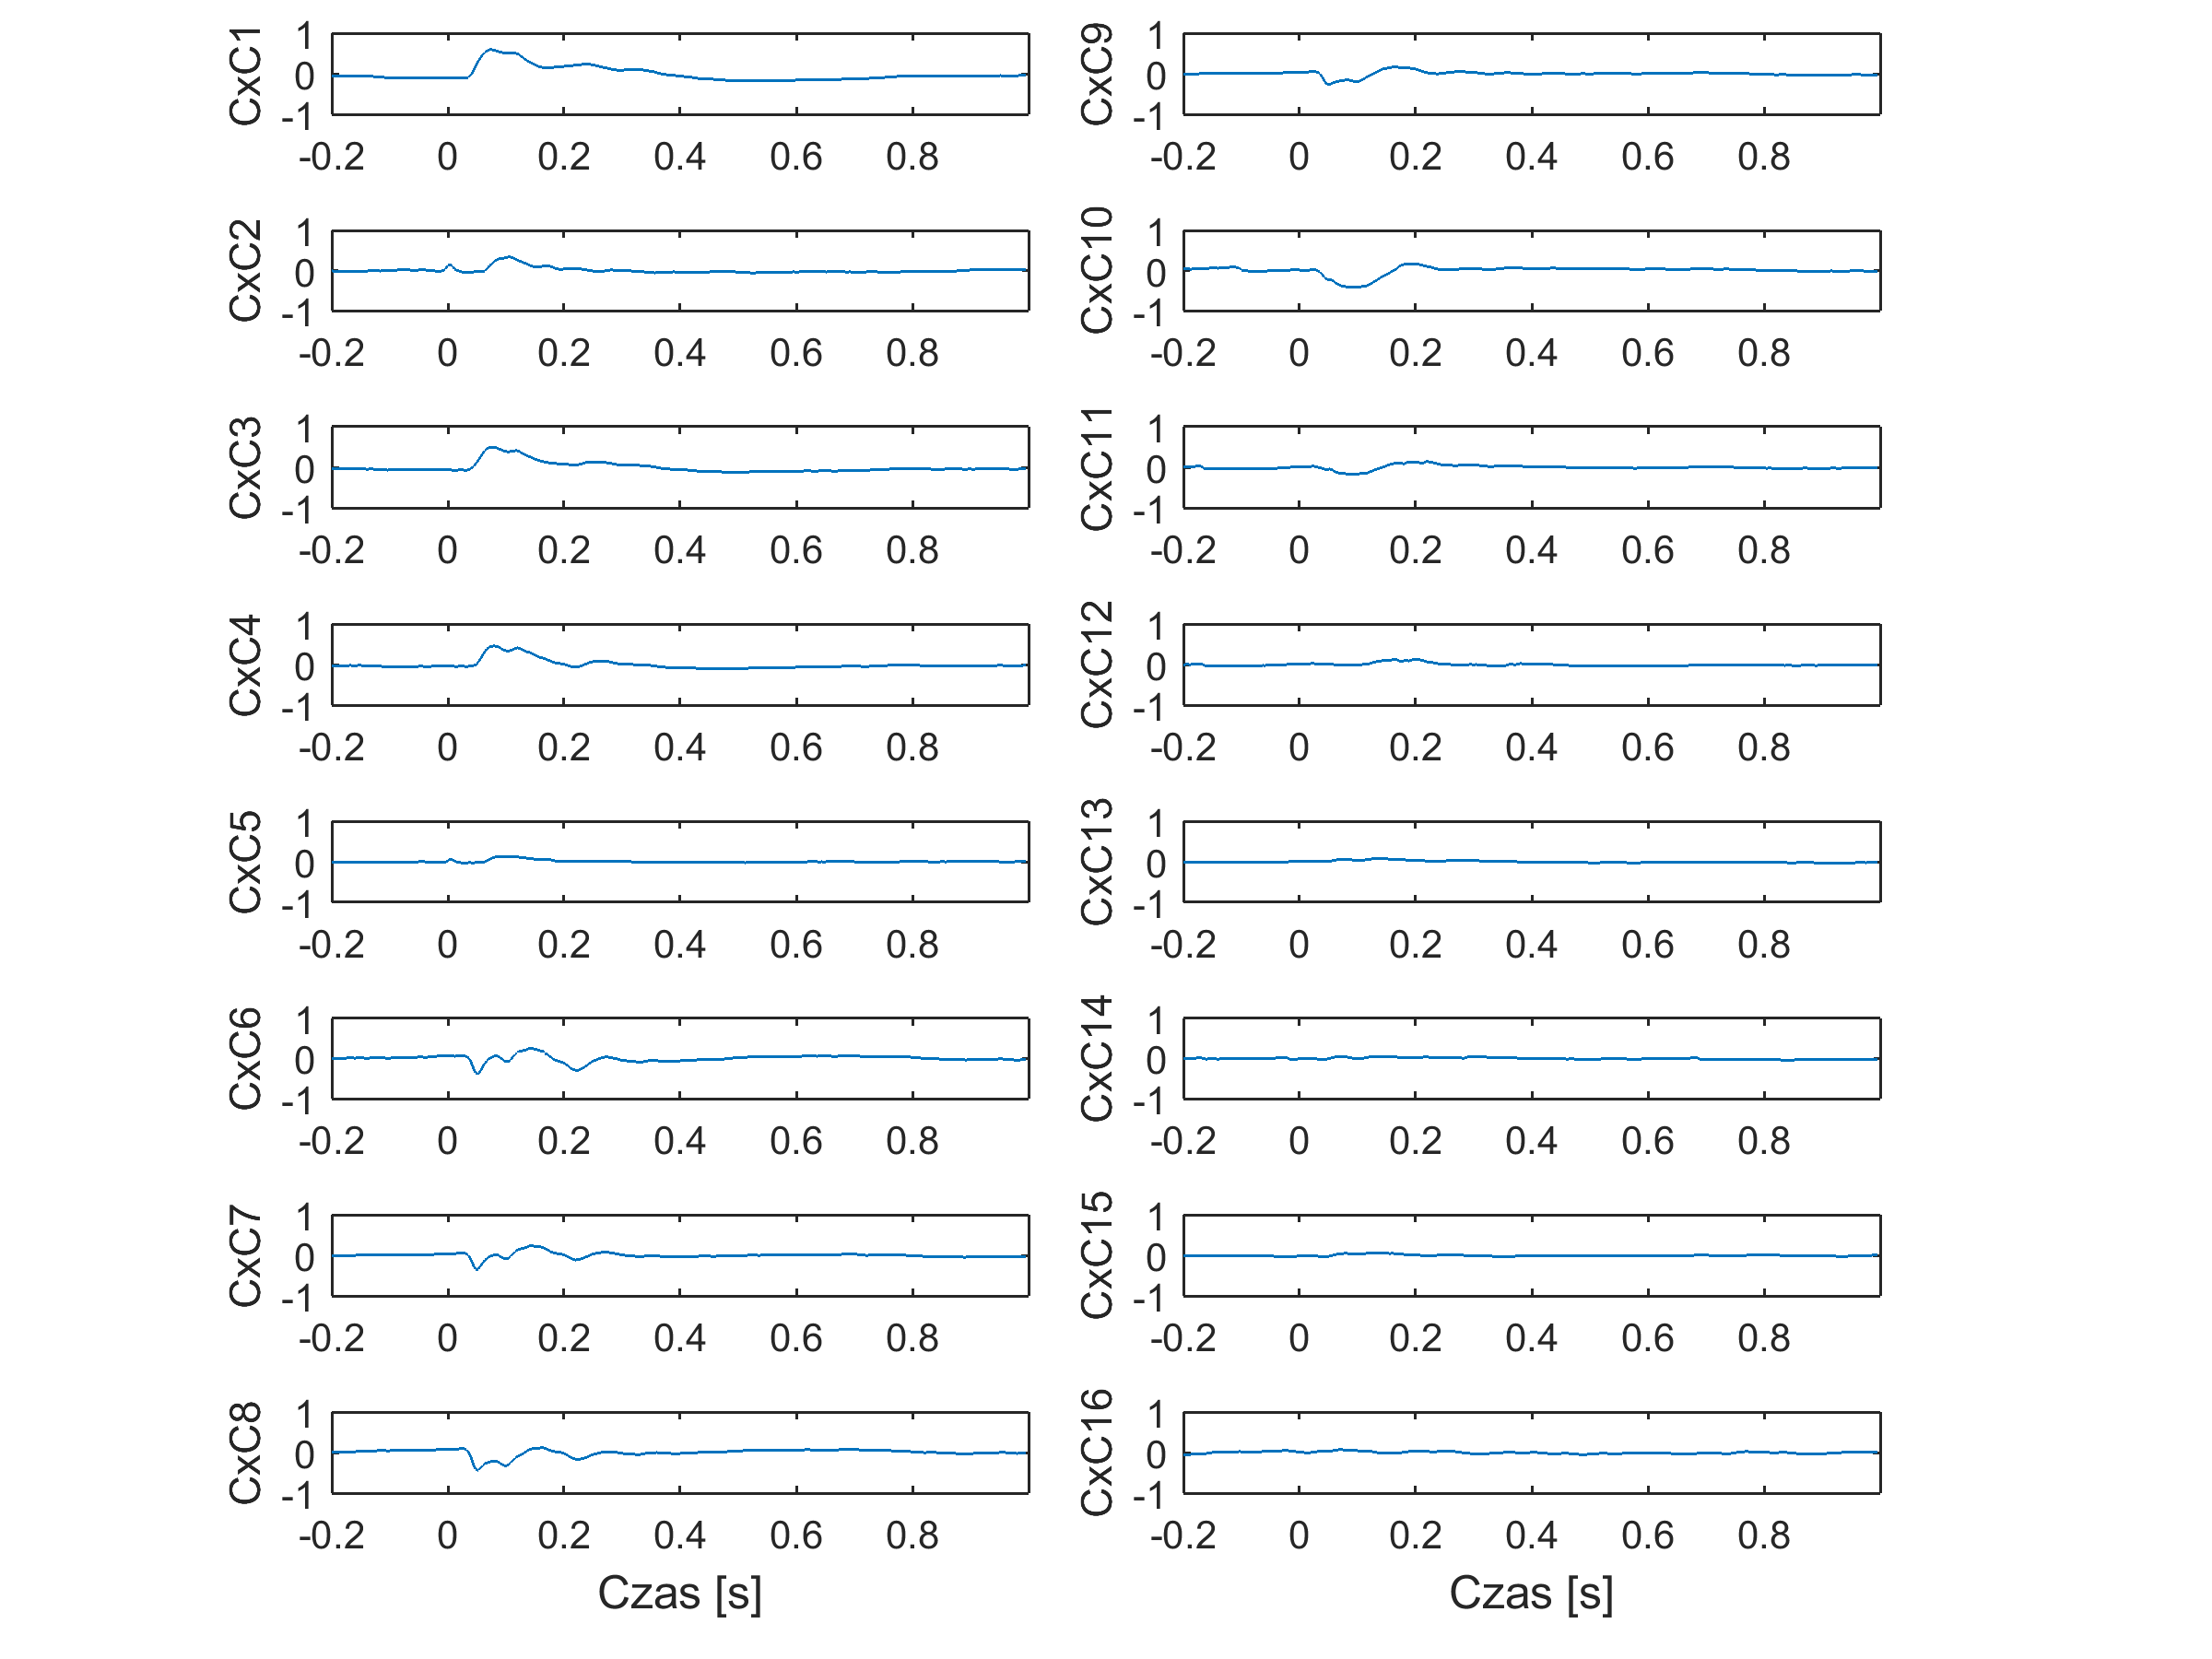
\includegraphics[width=\columnwidth]{16_kanalow.png}
		\end{center}
		\caption{Uśrednione potencjały wywołane z CxC dla danych kontrolnych z eksperymentu~A. Na kanale CxC2 widoczny jest artefakt od bodźca (pik w 0 s), natomiast na kanałach CxC12 -- CxC16 brak widocznej odpowiedzi na bodziec. Na kanale 5 można zaobserwować odwrócenie potencjału. Do dalszej analizy wybrano kanały CxC1, CxC4, CxC8 i CxC10.}
		\label{rys:16_kanalow}
	\end{figure}
	\newpage
	\section{Wielokanałowy model autoregresyjny}
	Sygnały pochodzące z rejestracji aktywności mózgu mogą być opisywane przez model AR (ang. \textit{autoregressive model}). Założeniem tego modelu jest to, $p + 1$ próbka powstaje jako kombinacja liniowa poprzednich $p$ próbek i niezależnej składowej losowej o średniej 0:
	\begin{equation}
		x(t) =  \sum_{i=1}^{p}a_ix(t-i) + e(t),
	\end{equation}
	gdzie $a_i$ jest $i$-tym współczynnikiem, a $e(t)$ -- składową szumową. \newline
	Jeśli podczas eksperymentu rejestruje się dane równocześnie z kilku źródeł, można przypuszczać, że są ze sobą związane. Wtedy sygnał z każdego źródła w $i$-tej chwili czasu traktuje się jak złożenie liniowe $p$ poprzednich próbek wszystkich źródeł:
	\begin{equation}
		\sum_{i=1}^{p}A(t)X(t-i) = E(t).
	\end{equation}
	Po przetransformowaniu powyższego równania do dziedziny częstości za pomocą transformacji~$Z$, otrzymuje się:
	\begin{equation}
		A(z)X(z) = E(z),
	\end{equation}
	gdzie podstawienie $z = e^{2\pi if\Delta t}$ daje przejście do funkcji zależnej od częstości.
	
	Macierz wariancji szumów $V$ można zapisać:
	\begin{equation}
		V = E(f)*E(f)^{+},
	\end{equation}
	Znak $^{+}$ oznacza transpozycję macierzy połączoną ze sprzężeniem zespolonym jej elementów.
	Dla określenia rzędu modelu ($p$) stosuje się różnego rodzaju kryteria. Jednym z nich jest kryterium Akaikego \citep[s. 79]{jarek}:
	\begin{equation}
		AIC(p) = ln(det(V))+2\frac{pk^2}{N}.
	\end{equation}
	\section{Połączenia funkcjonalne}
	Zależności między dostępnymi kanałami (dane z kilku źródeł zbierane równocześnie) można badać na wiele sposobów. Jedną z podstawowych miar podobieństwa między kanałami jest koherencja. Wadą tej funkcji jest to, że nie pozwala stwierdzić kierunku oddziaływania między danymi źródłowymi. Żeby móc odpowiedzieć na pytanie, który kanał generuje informację, a który ją tylko odbiera, skorzystano z kierunkowej funkcji przejścia, bazującej na przyczynowości w sensie Grangera.
	
	\subsection{Przyczynowość w sensie Grangera}
	Definicja przyczynowości bazuje na przewidywalności szeregów czasowych. Przy założeniu, że wartość sygnału x da się przewidzieć na podstawie $p$ poprzednich wartości otrzymuje się:
	\begin{equation}
		X(t) = \sum_{i=1}^{p}A_1(i)x(t-i)+E_1(t),
	\end{equation}
	gdzie $A_1$ jest macierzą współczynników, a $E_1$ -- macierzą wartości szumowych.
	
	Macierz wartości szumowych można traktować jako miarę dopasowania -- im czynnik szumowy jest mniejszy, tym dane są lepiej opisywane przez model.
	
	Przy założeniu, że na wartość sygnału x ma również wpływ sygnał y, można zapisać:
	\begin{equation}
		X(t) = \sum_{i=1}^{p}A_1(i)x(t-i)+\sum_{i=1}^{p}A_2(i)y(t-i)+E_2(t).
	\end{equation}
	Jeśli var$(E_1)$ $>$ var$(E_2)$, to można powiedzieć, że w sensie przyczynowości Grangera sygnał x jest zależny od sygnału y. W przypadku gdy obie wartości są porównywalne to znaczy, że dodatkowa informacja o wartościach sygnału y nie wniosła nic do opisu wartości sygnału x, a więc sygnał x jest niezależny od sygnału y.
	\subsection{Kierunkowa funkcja przejścia -- opis metody}
	Kierunkowa funkcja przejścia (z ang. \textit{Direct Transfer Function}) opiera się o założenie, że dane są dobrze opisywane przez wielokanałowy model autoregresyjny (MVAR). Definiuje się ją przez macierz przejścia modelu $H$ daną wzorem: $H = A^{-1}$.
	
	Kierunkowa funkcja przejścia w wersji nieznormalizowanej:
	\begin{equation}
		{NDTF}_{i\to j}^2 (f) = {\left|H_{ij}(f) \right|}^2
	\end{equation}
	Znormalizowana kierunkowa funkcja przejścia:
	\begin{equation}
		{DTF}_{i\to j}^2 (f) = \frac{{\left|H_{ij}(f) \right|}^2}{\sum_{m=1}^{k}{\left|H_{im}(f) \right|}^2 }
	\end{equation}
	\subsection{Zastosowanie metody}
	Dla danych z obu eksperymentów wybrano model 4 rzędu na podstawie kryterium Akaikego. Dla wybranych 13 kanałów policzono NDTF w czasie, gdzie rozmiar okna wynosił 25 próbek, a przesunięcie -- 5. Następnie wybrano trzy zakresy częstości, w których analizowano sygnał: 
	\begin{itemize}
		\item {[1-10]} Hz
		\item {[10-30]} Hz
		\item {[20-40]} Hz
	\end{itemize}
	\subsection{Statystyka}\label{NDTF}
	Istotność statystyczną sprawdzano na postawie bootstrapu. Dla każdej pary kanałów 100-krotnie losowano z powtórzeniami 200 realizacji i obliczano rozkład wartości funkcji NDTF. Następnie dla każdego zakresu, spośród wszystkich częstości w nim zawartych, wybierano najwyższą wartość odpowiadającą 97,5 percentylowi oraz najniższą -- 2,5 percentylowi. Otrzymano w ten sposób 95\%-owe przedziały ufności dla każdego zakresu częstości.
	\chapter{Wyniki}
	\section{Uśrednianie potencjałów}
	Na Rysunku \ref{rys:usrednione_CxC} przedstawiono uśrednianie potencjałów dla danych z eksperymentu A z~kontralateralnej kory wzrokowej przed treningiem wzrokowym. Przed uśrednieniem dane zawierają duży wkład od czynności spontanicznej, która maskuje potencjał wywołany i dopiero po uśrednieniu uwidacznia się kształt odpowiedzi na bodziec. Pomiędzy kanałami CxC4 i CxC8 widoczna jest zmiana polaryzacji.
	\begin{figure}[htbp]
		\begin{center}
			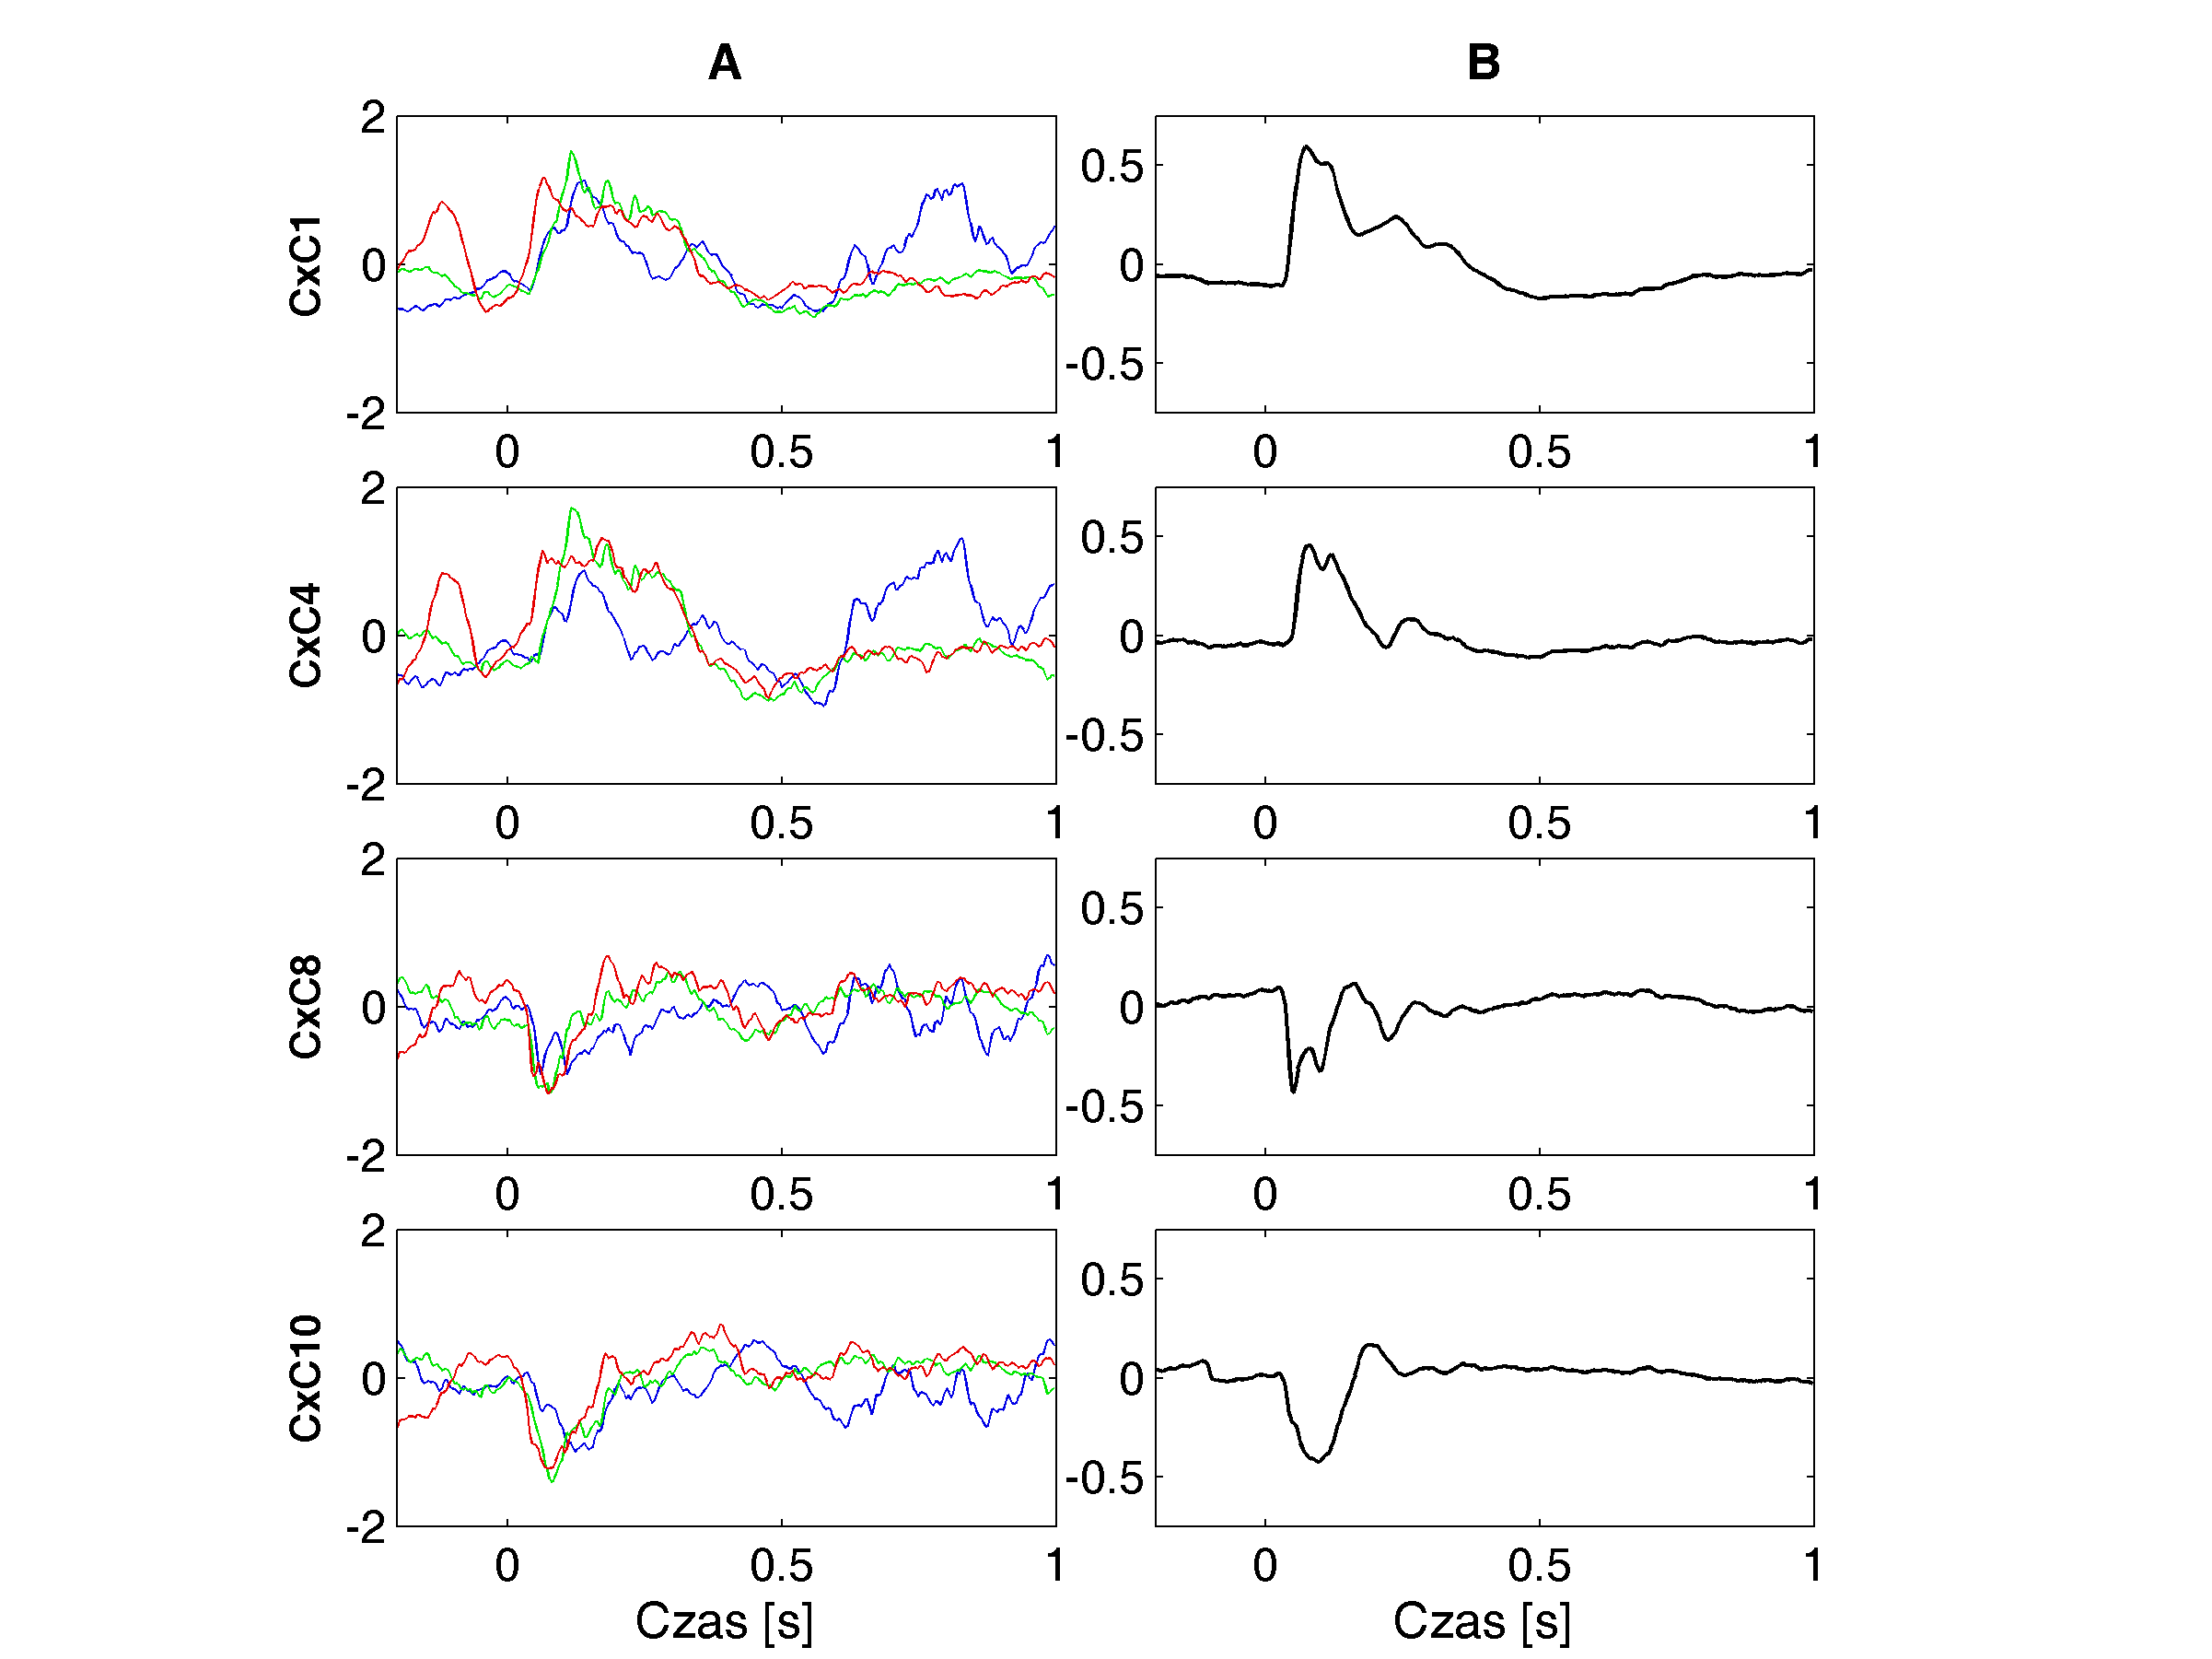
\includegraphics[scale=0.65]{usrednione_CxC.png}
		\end{center}
		\caption{Porównanie pojedynczych i uśrednionych realizacji dla 4 wybranych kanałów z CxC. W kolumnie A przedstawiono 3 pojedyncze powtórzenia, a w kolumnie B -- uśrednione po wszystkich realizacjach potencjały wywołane.}
		\label{rys:usrednione_CxC}
	\end{figure}
	\FloatBarrier
	\subsection{Porównanie uśrednionych potencjałów z CxC}
	Na Rysunkach \ref{rys:kontrola15_CxC} i \ref{rys:beta3_CxC} przedstawiono uśrednione po realizacjach potencjały wywołane dla różnych długości treningu odpowiednio dla danych z eksperymentu A (Rysunek \ref{rys:kontrola15_CxC}) i eksperymentu B (Rysunek \ref{rys:beta3_CxC}).
	\begin{figure}[htbp]
		\begin{center}
			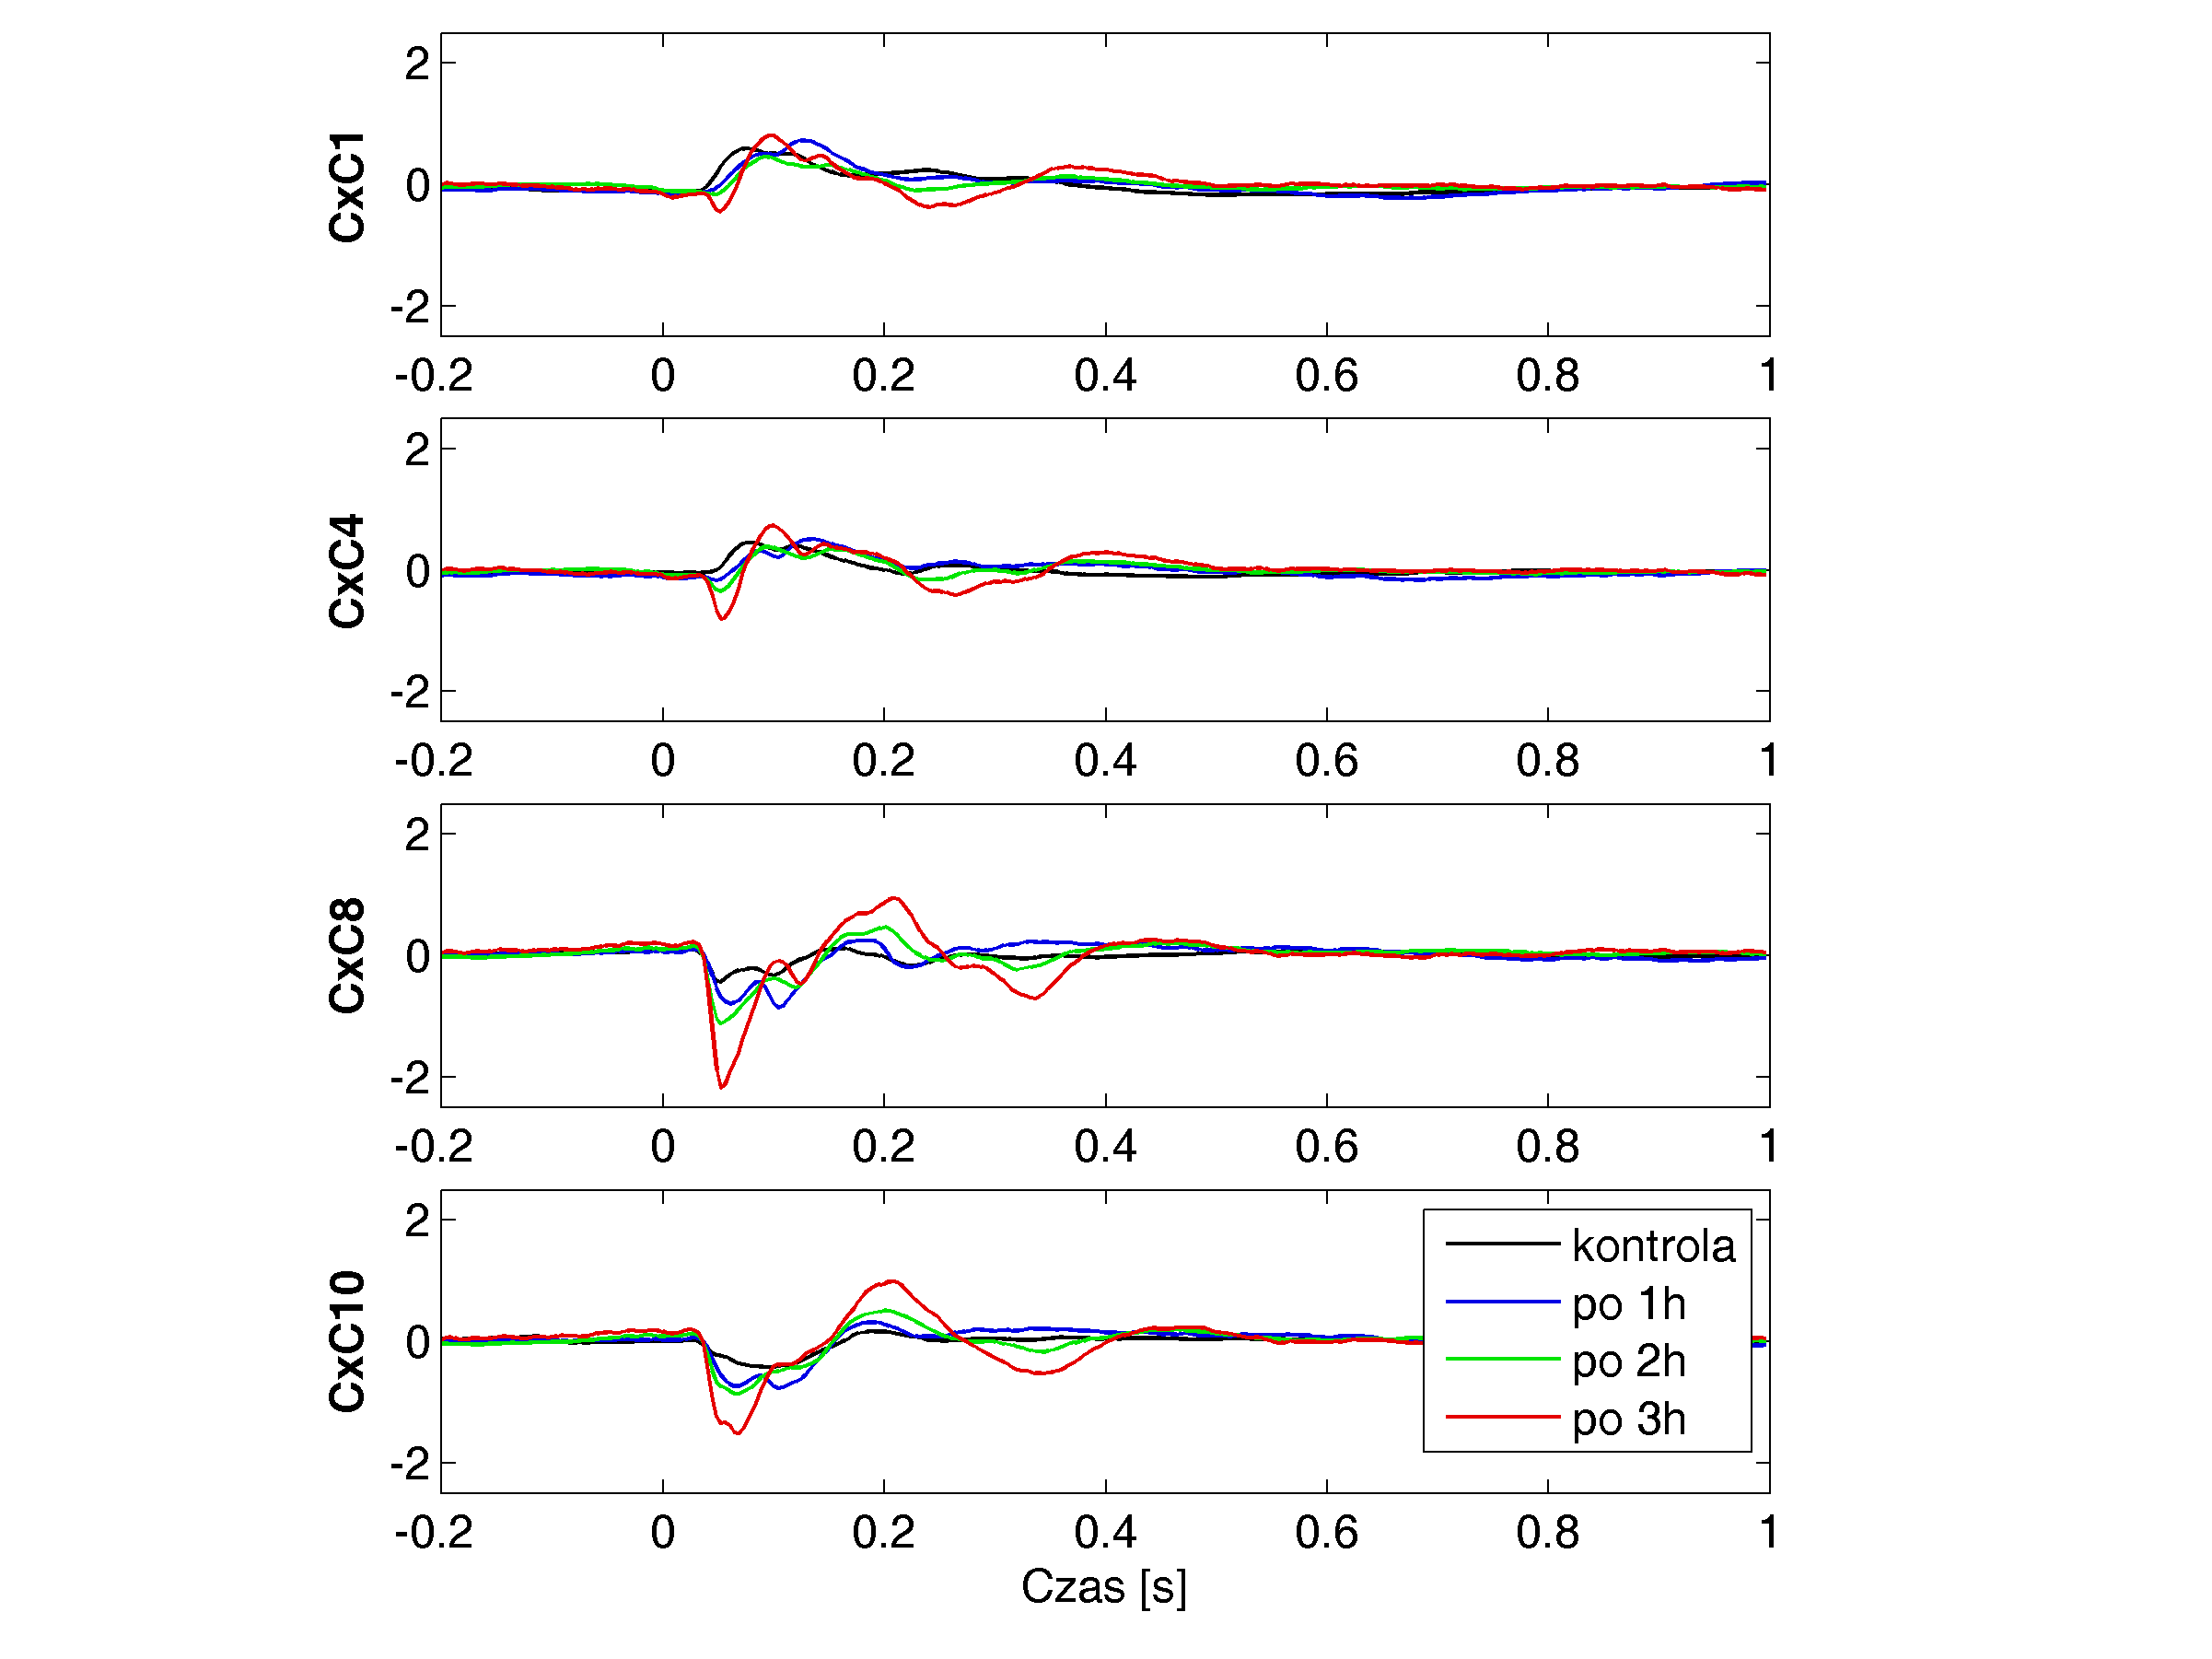
\includegraphics[scale=0.8]{kontrola15_CxC.png}
		\end{center}
		\caption{Eksperyment A: Uśrednione po realizacjach potencjały wywołane. Kolorami zaznaczono kolejne godziny treningu.}
		\label{rys:kontrola15_CxC}
	\end{figure}
	\FloatBarrier
	Na obu wykresach widoczne jest zwiększanie się amplitudy odpowiedzi na bodziec wraz z długością treningu wzrokowego.
	\begin{figure}[h]
		\begin{center}
			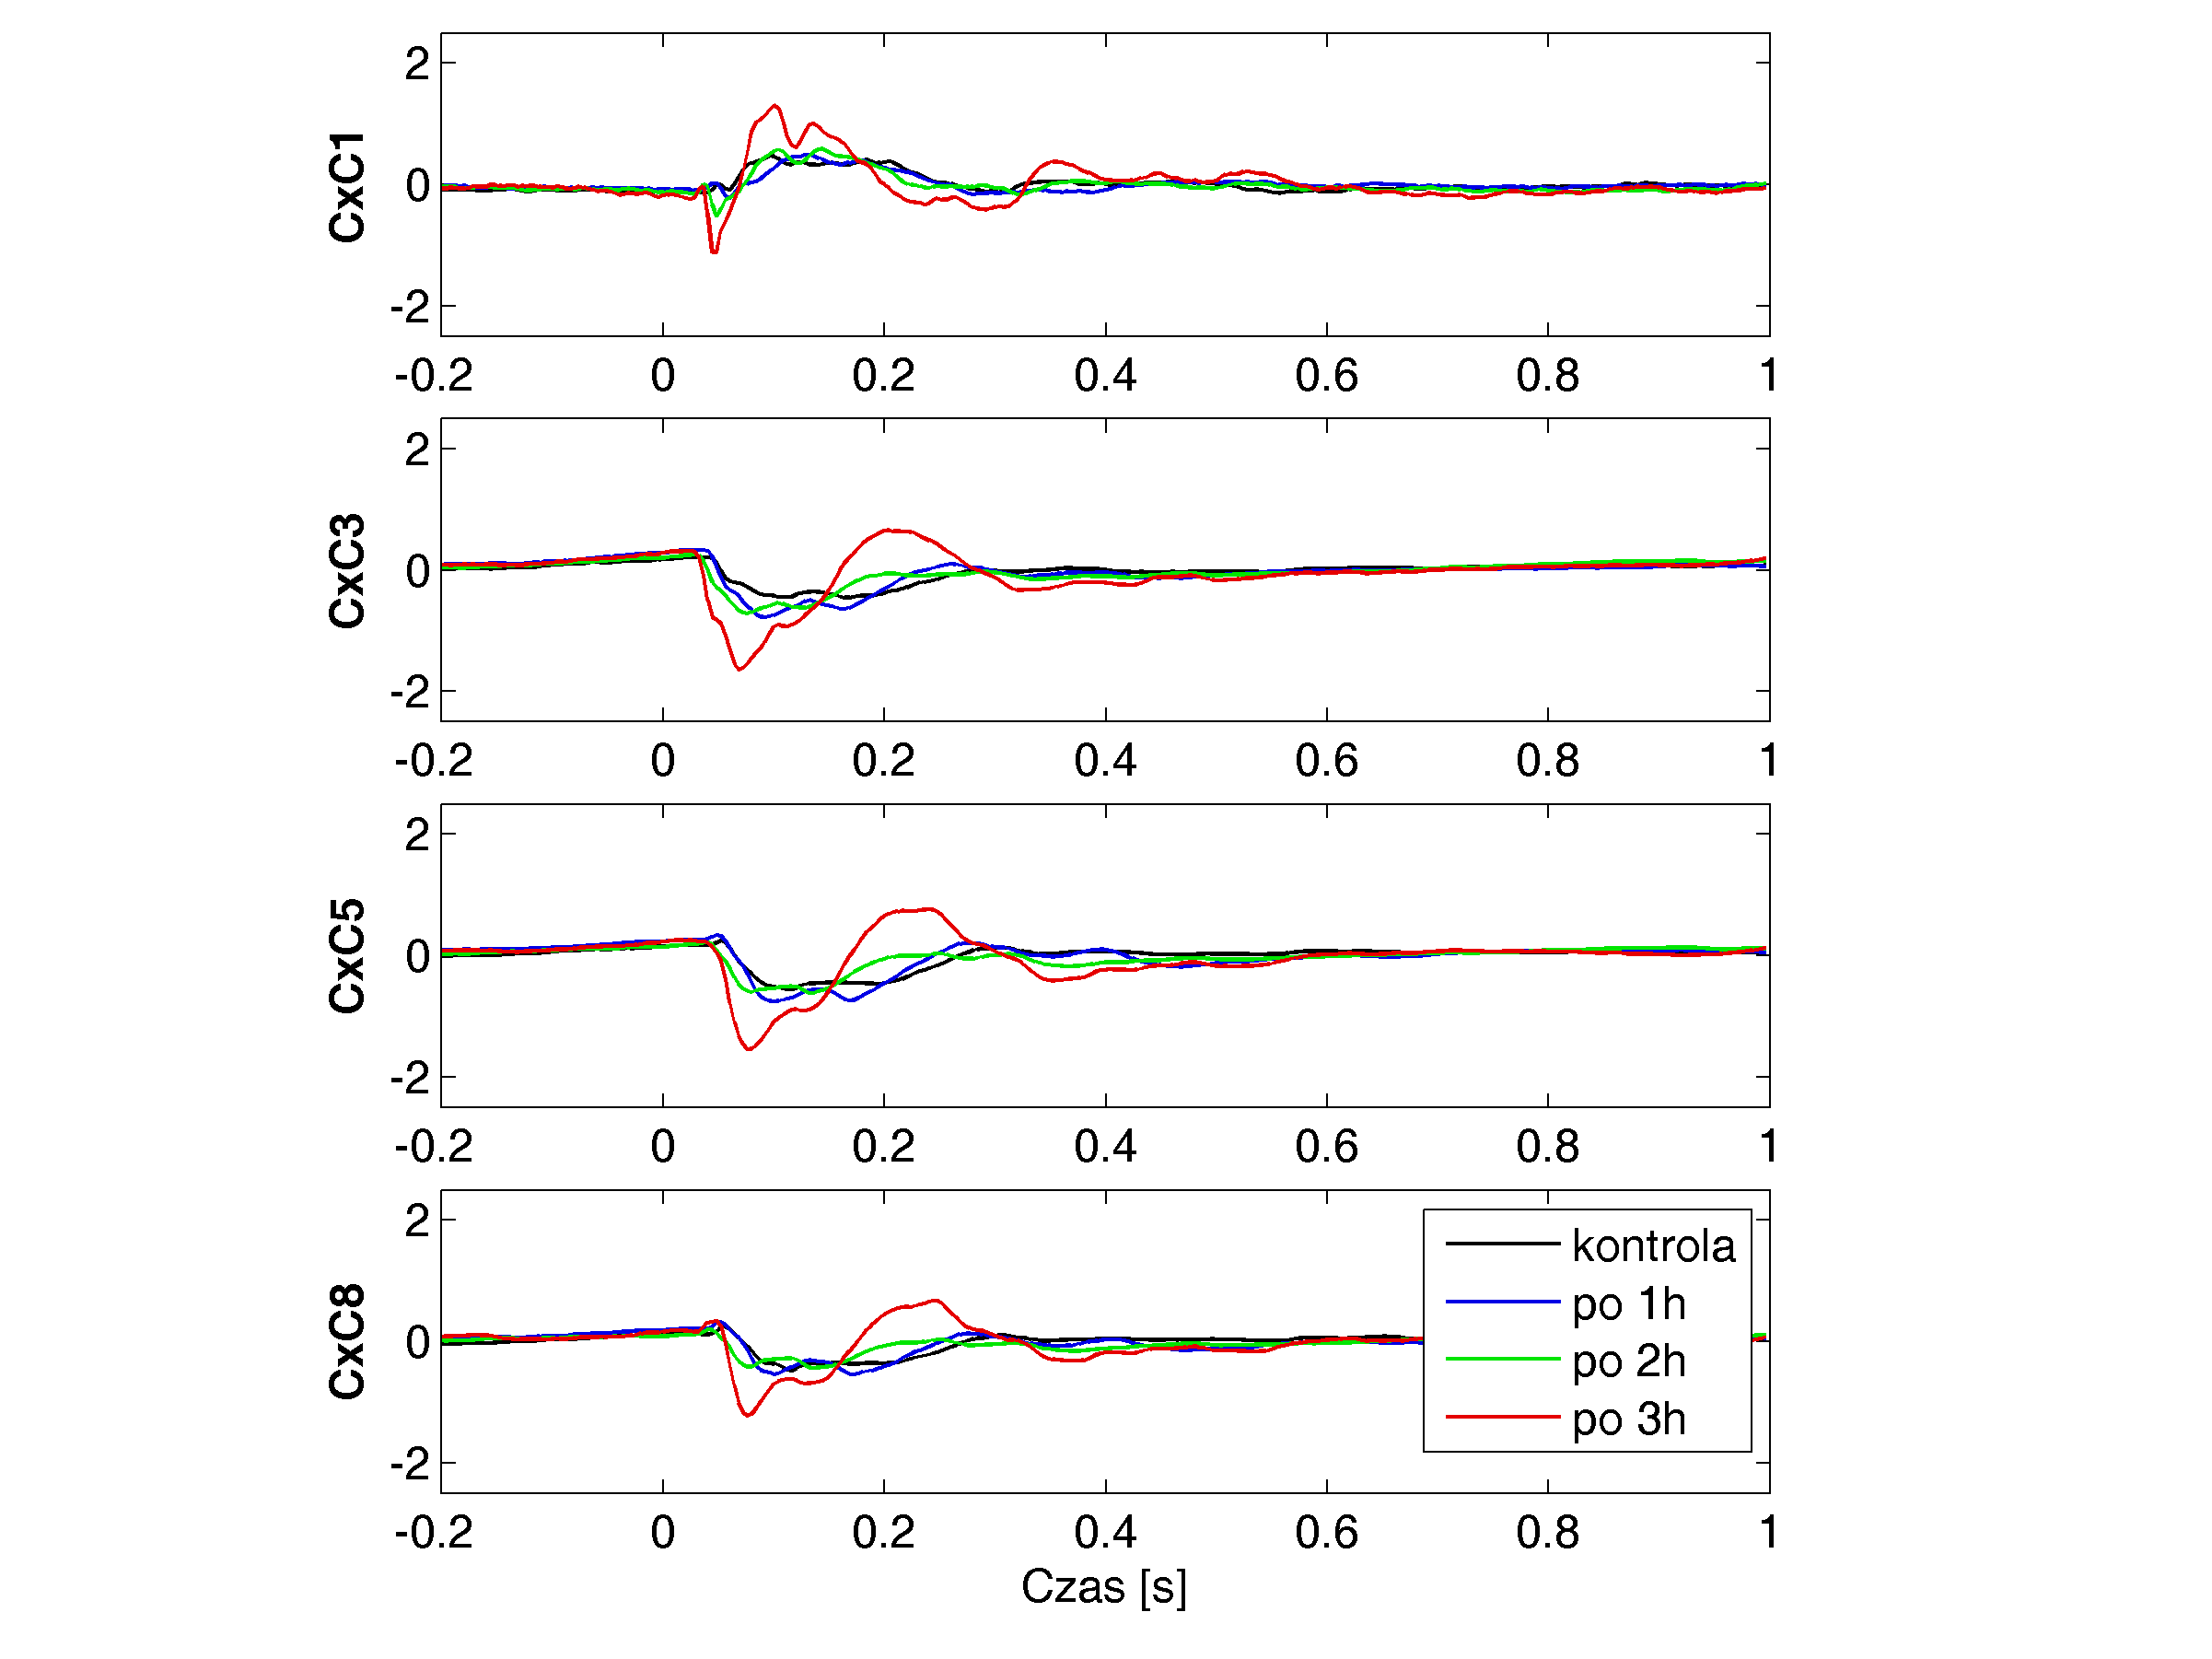
\includegraphics[scale=0.8]{beta3_CxC.png}
		\end{center}
		\caption{Eksperyment B: Uśrednione po realizacjach potencjały wywołane. Kolorami zaznaczono kolejne godziny treningu.}
		\label{rys:beta3_CxC}
	\end{figure}
	\FloatBarrier 
	Aby sprawdzić, czy zwiększenie jest rzeczywiście istotne, przeprowadzono analizę statystyczną zgodnie z opisem zamieszczonym w Sekcji \ref{statystyka}.
		
	Wyniki testów zamieszczono w Tabeli \ref{tab:kontrola_CxC_P} dla eksperymentu A i w Tabeli \ref{tab:beta_CxC_P} dla eksperymentu~B.
	\begin{table}[htdp]
		\caption{P wartości dla CxC z eksperymentu A.}
		\begin{center}
			\begin{tabularx}{0.9\textwidth}{l C C C C}
				\toprule
				\textbf{} & \textbf{CxC1} & \textbf{CxC4} & \textbf{CxC8} & \textbf{CxC10}
				\\
				\midrule
				kontrola vs po 1 h & 0,706 & 0,612 & 0,001 & 0,001\\
				kontrola vs po 2 h & 0,994 & 0,001 & 0,001 & 0,001\\
				kontrola vs po 3 h & 0,001 & 0,001 & 0,001 & 0,001\\
				\bottomrule
			\end{tabularx}
		\end{center}
		\label{tab:kontrola_CxC_P}
	\end{table}
	
	\begin{table}[htdp]
		\caption{P wartości dla CxC z eksperymentu B.}
		\begin{center}
			\begin{tabularx}{0.9\textwidth}{l C C C C}
				\toprule
				\textbf{} & \textbf{CxC1} & \textbf{CxC3} & \textbf{CxC5} & \textbf{CxC6} \\
				\midrule
				kontrola vs po 1 h & 0,955 & 0,001 & 0,001 & 0,001\\
				kontrola vs po 2 h & 0,001 & 0,001 & 0,127 & 0,134\\
				kontrola vs po 3 h & 0,001 & 0,001 & 0,001 & 0,001\\
				\bottomrule
			\end{tabularx}
		\end{center}
		\label{tab:beta_CxC_P}
	\end{table}
	\FloatBarrier
	Na podstawie tych wyników można stwierdzić, że wzrost amplitudy wraz z długością treningu wzrokowego jest istotny statystycznie. Nie da się jednak jednoznacznie określić, że stymulacja elektryczna w eksperymencie B przyczyniła się do zwiększenia amplitudy między kontrolą a kolejnymi rejestracjami.
	\subsection{Porównanie uśrednionych potencjałów z CxI}\label{CxI}
	Na Rysunkach \ref{rys:kontrola15_CxI} i \ref{rys:beta3_CxI} przedstawiono uśrednione potencjały wywołane odpowiednio dla danych z eksperymentu A i B.
	
	W zestawie danych z eksperymentu A są widoczne artefakty od bodźców (Rysunek \ref{rys:kontrola15_CxI}). Natomiast uśrednione potencjały wywołane z eksperymentu B (Rysunek \ref{rys:beta3_CxI}) nie mają typowego kształtu. 
	
	\begin{figure}[h]
		\begin{center}
			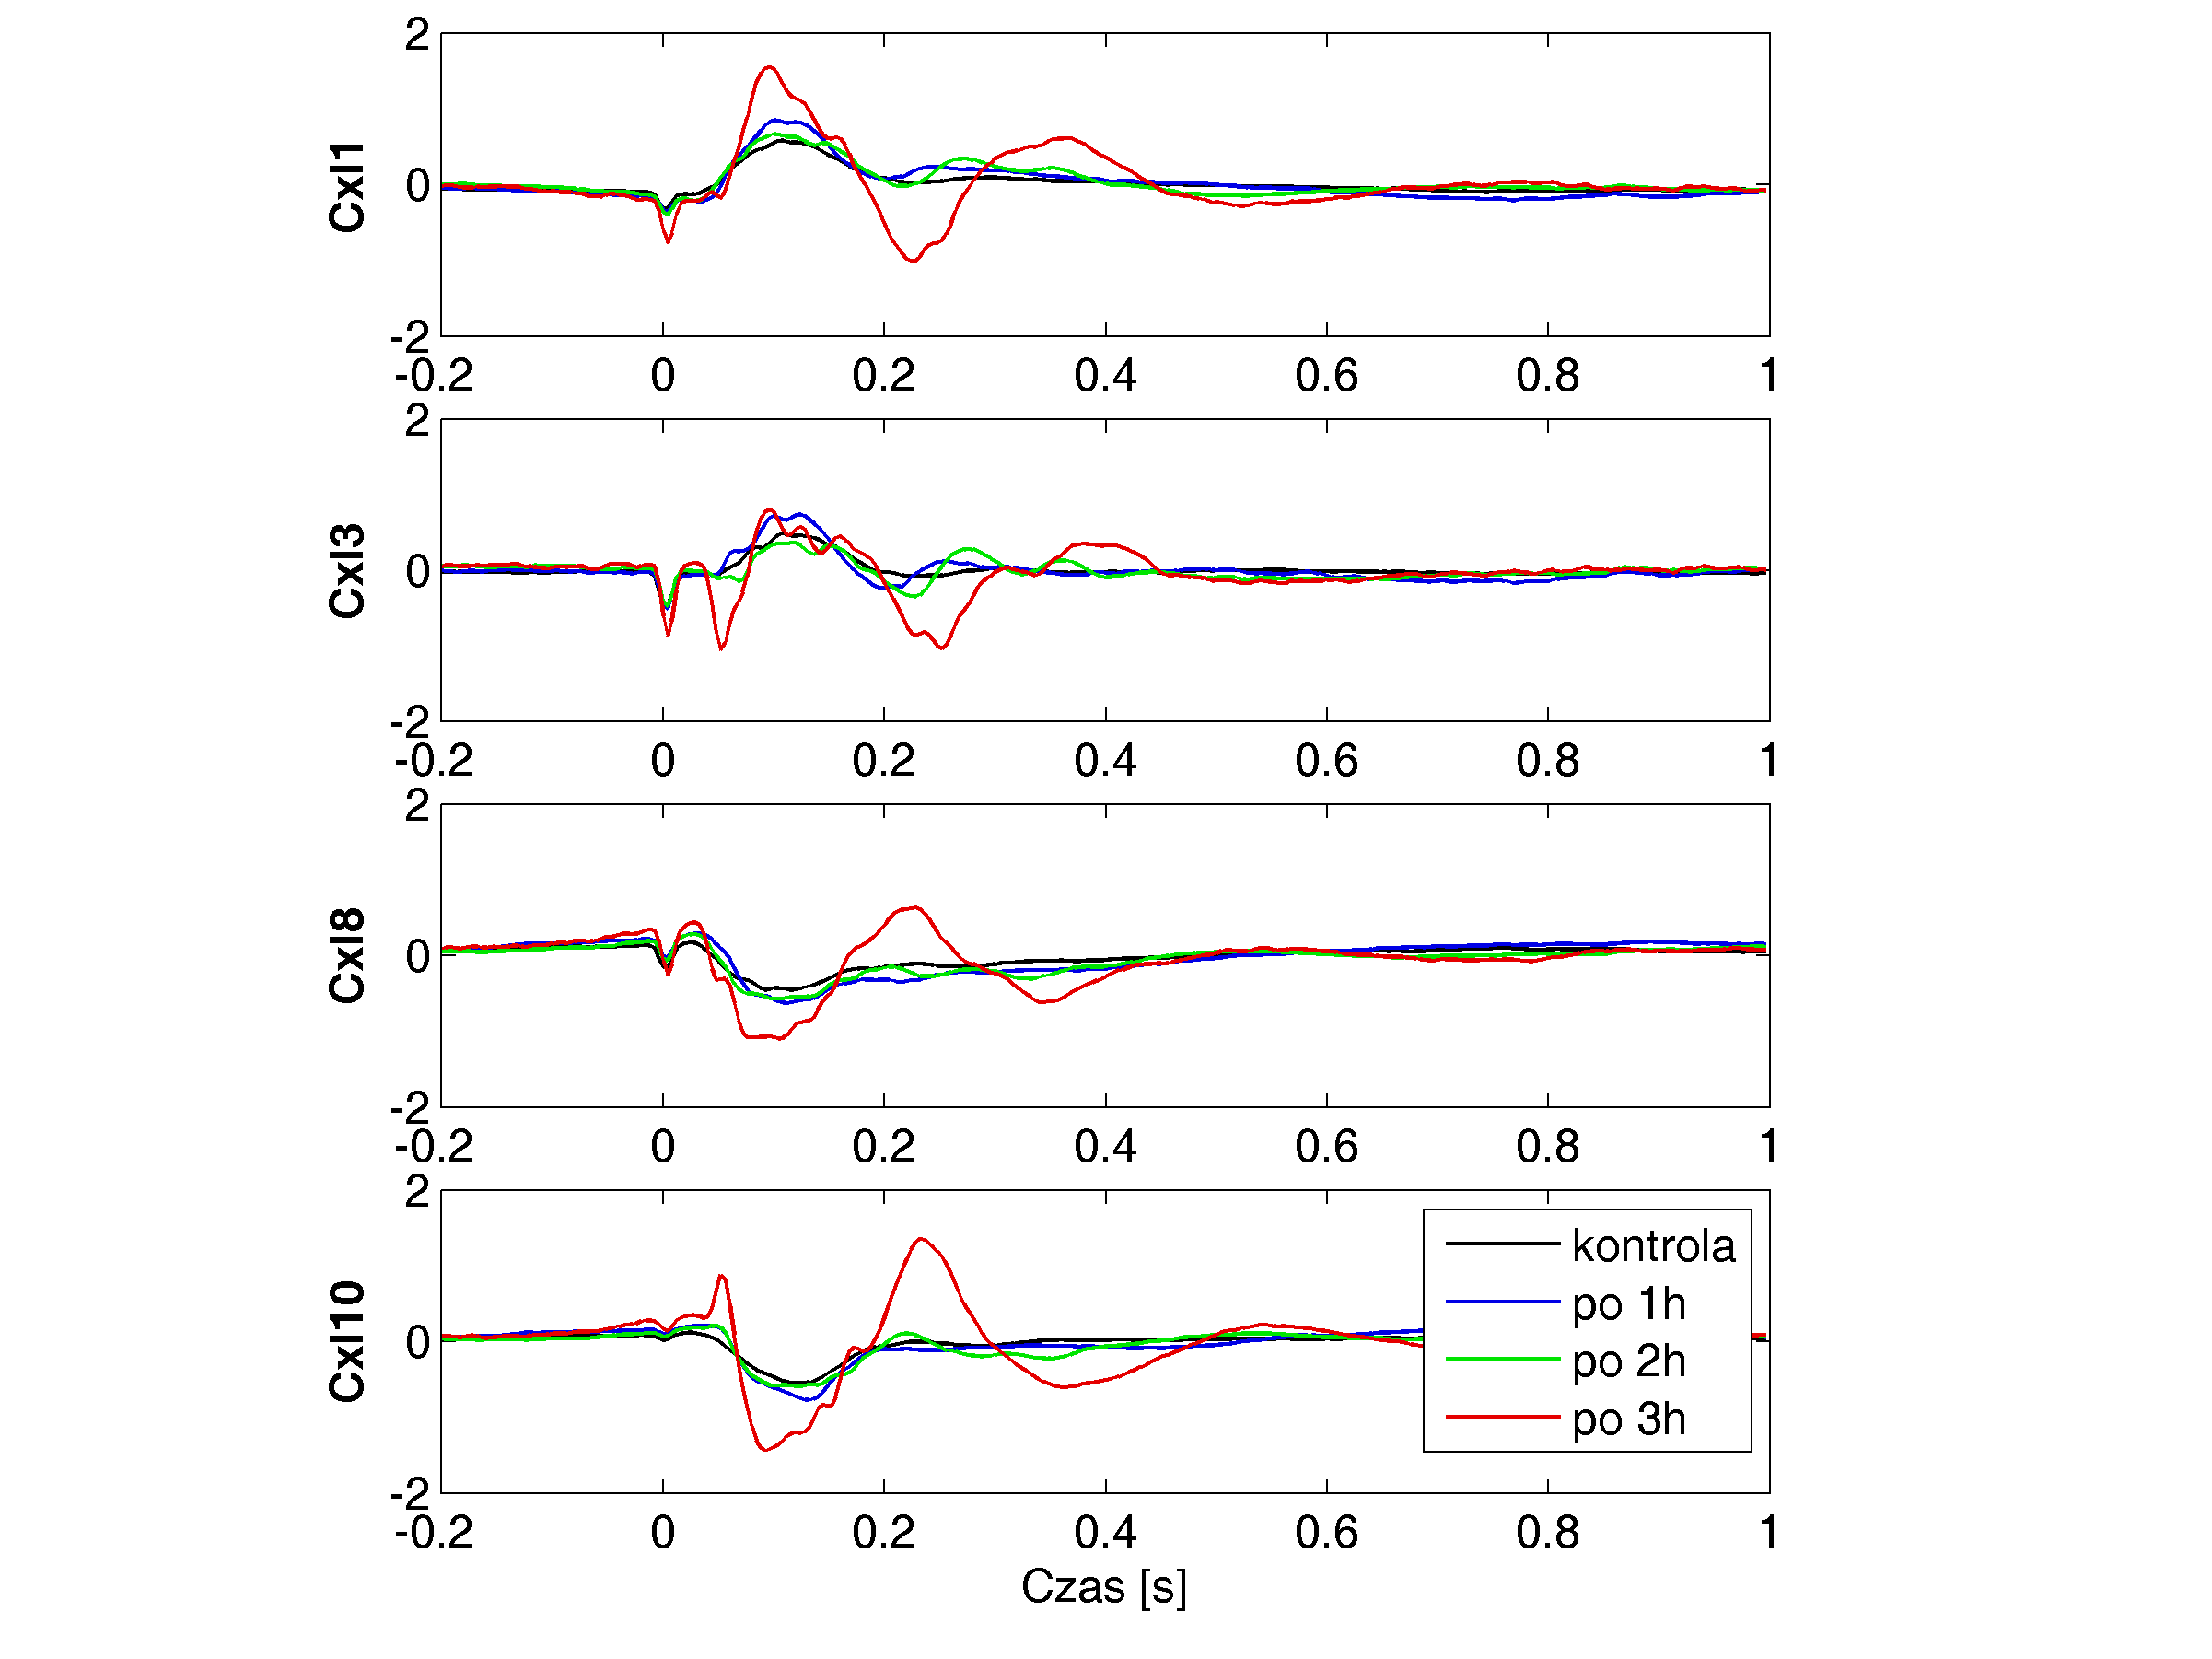
\includegraphics[scale=0.8]{kontrola15_CxI.png}
		\end{center}
		\caption{Eksperyment A: Uśrednione po realizacjach potencjały wywołane. Kolorami zaznaczono kolejne godziny treningu.}
		\label{rys:kontrola15_CxI}
	\end{figure}
	\FloatBarrier
	\begin{figure}[h]
		\begin{center}
			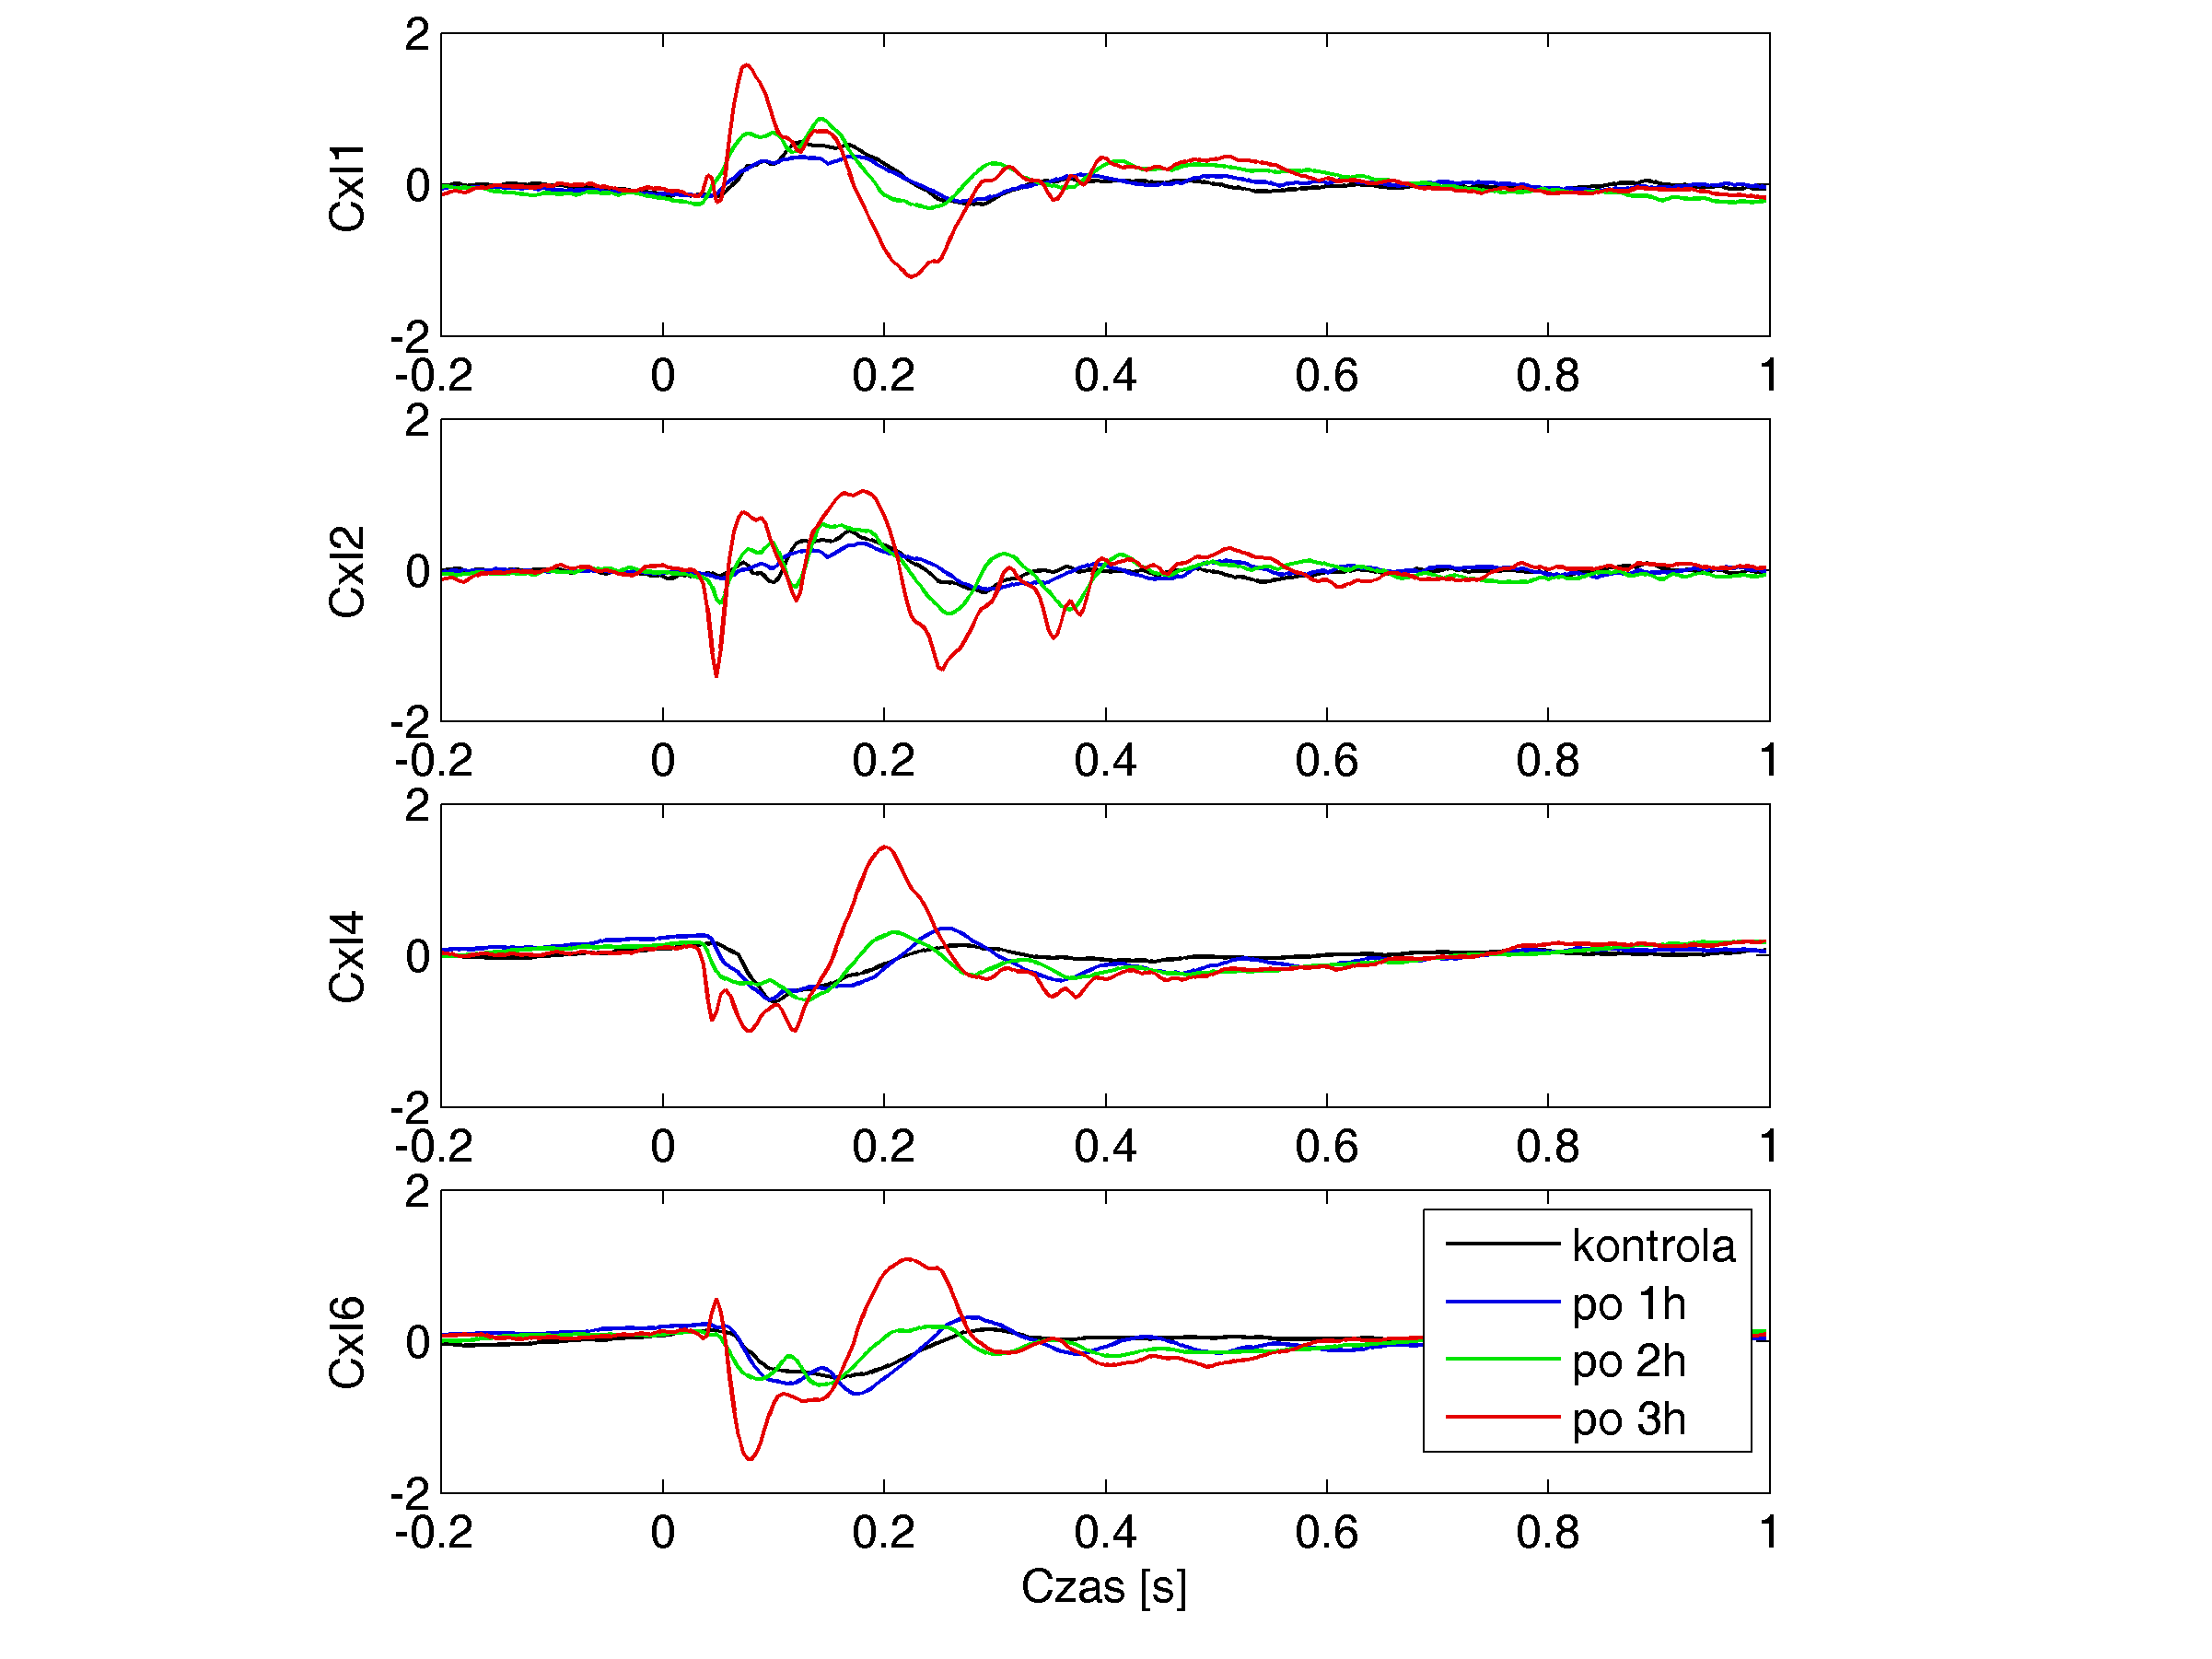
\includegraphics[scale=0.8]{beta3_CxI.png}
		\end{center}
		\caption{Eksperyment B: Uśrednione po realizacjach potencjały wywołane. Kolorami zaznaczono kolejne godziny treningu.}
		\label{rys:beta3_CxI}
	\end{figure}
	\FloatBarrier
	W Tabelach \ref{tab:kontrola_CxI_P} i \ref{tab:beta_CxI_P} zestawiono wartości statystyki dla obu eksperymentów. Dla danych z eksperymentu A wzrost amplitudy jest bardziej istotny statystyczne niż dla danych z eksperymentu B. Jest to prawdopodobnie  spowodowane nietypowym kształtem potencjałów wywołanych dla danych z zestawu B.
	\begin{table}[htdp]
		\caption{P wartości dla CxI z eksperymentu A.}
		\begin{center}
			\begin{tabularx}{0.9\textwidth}{l C C C C}
				\toprule
				\textbf{} & \textbf{CxI1} & \textbf{CxI3} & \textbf{CxI8} & \textbf{CxI10} \\
				\midrule
				kontrola vs po 1 h & 0,001 & 0,001 & 0,001 & 0,002\\
				kontrola vs po 2 h & 0,709 & 0,001 & 0,001 & 0,003\\
				kontrola vs po 3 h & 0,001 & 0,001 & 0,001 & 0,001\\
				\bottomrule
			\end{tabularx}
		\end{center}
		\label{tab:kontrola_CxI_P}
	\end{table}
	\FloatBarrier
		\begin{table}[htdp]
			\caption{P wartości dla CxI z eksperymentu B.}
			\begin{center}
				\begin{tabularx}{0.9\textwidth}{l C C C C}
					\toprule
					\textbf{} & \textbf{CxI1} & \textbf{CxI2} & \textbf{CxI4} & \textbf{CxI6} \\
					\midrule
					kontrola vs po 1 h & 0,506 & 0,670 & 0,115 & 0,001\\
					kontrola vs po 2 h & 0,001 & 0,001 & 1     & 0,042\\
					kontrola vs po 3 h & 0,001 & 0,001 & 0,001 & 0,001\\
					\bottomrule
				\end{tabularx}
			\end{center}
			\label{tab:beta_CxI_P}
		\end{table}
	\FloatBarrier
	\subsection{Porównanie uśrednionych potencjałów z SC}\label{SC}
	Na Rysunkach \ref{rys:kontrola15_SC} i \ref{rys:beta3_SC} przedstawiono uśrednione potencjały wywołane dla obu zestawów danych. Dla danych z eksperymentu A jest widoczne odwrócenie polaryzacji między kanałami SC2 i SC4 (Rysunek \ref{rys:kontrola15_SC}), czego nie udało się zaobserwować dla SC z eksperymentu B (Rysunek \ref{rys:beta3_SC}). Można więc podejrzewać, że elektroda została wbita zbyt głęboko i nie udało się zarejestrować płytszych warstw.
	\begin{figure}[htbp]
		\begin{center}
			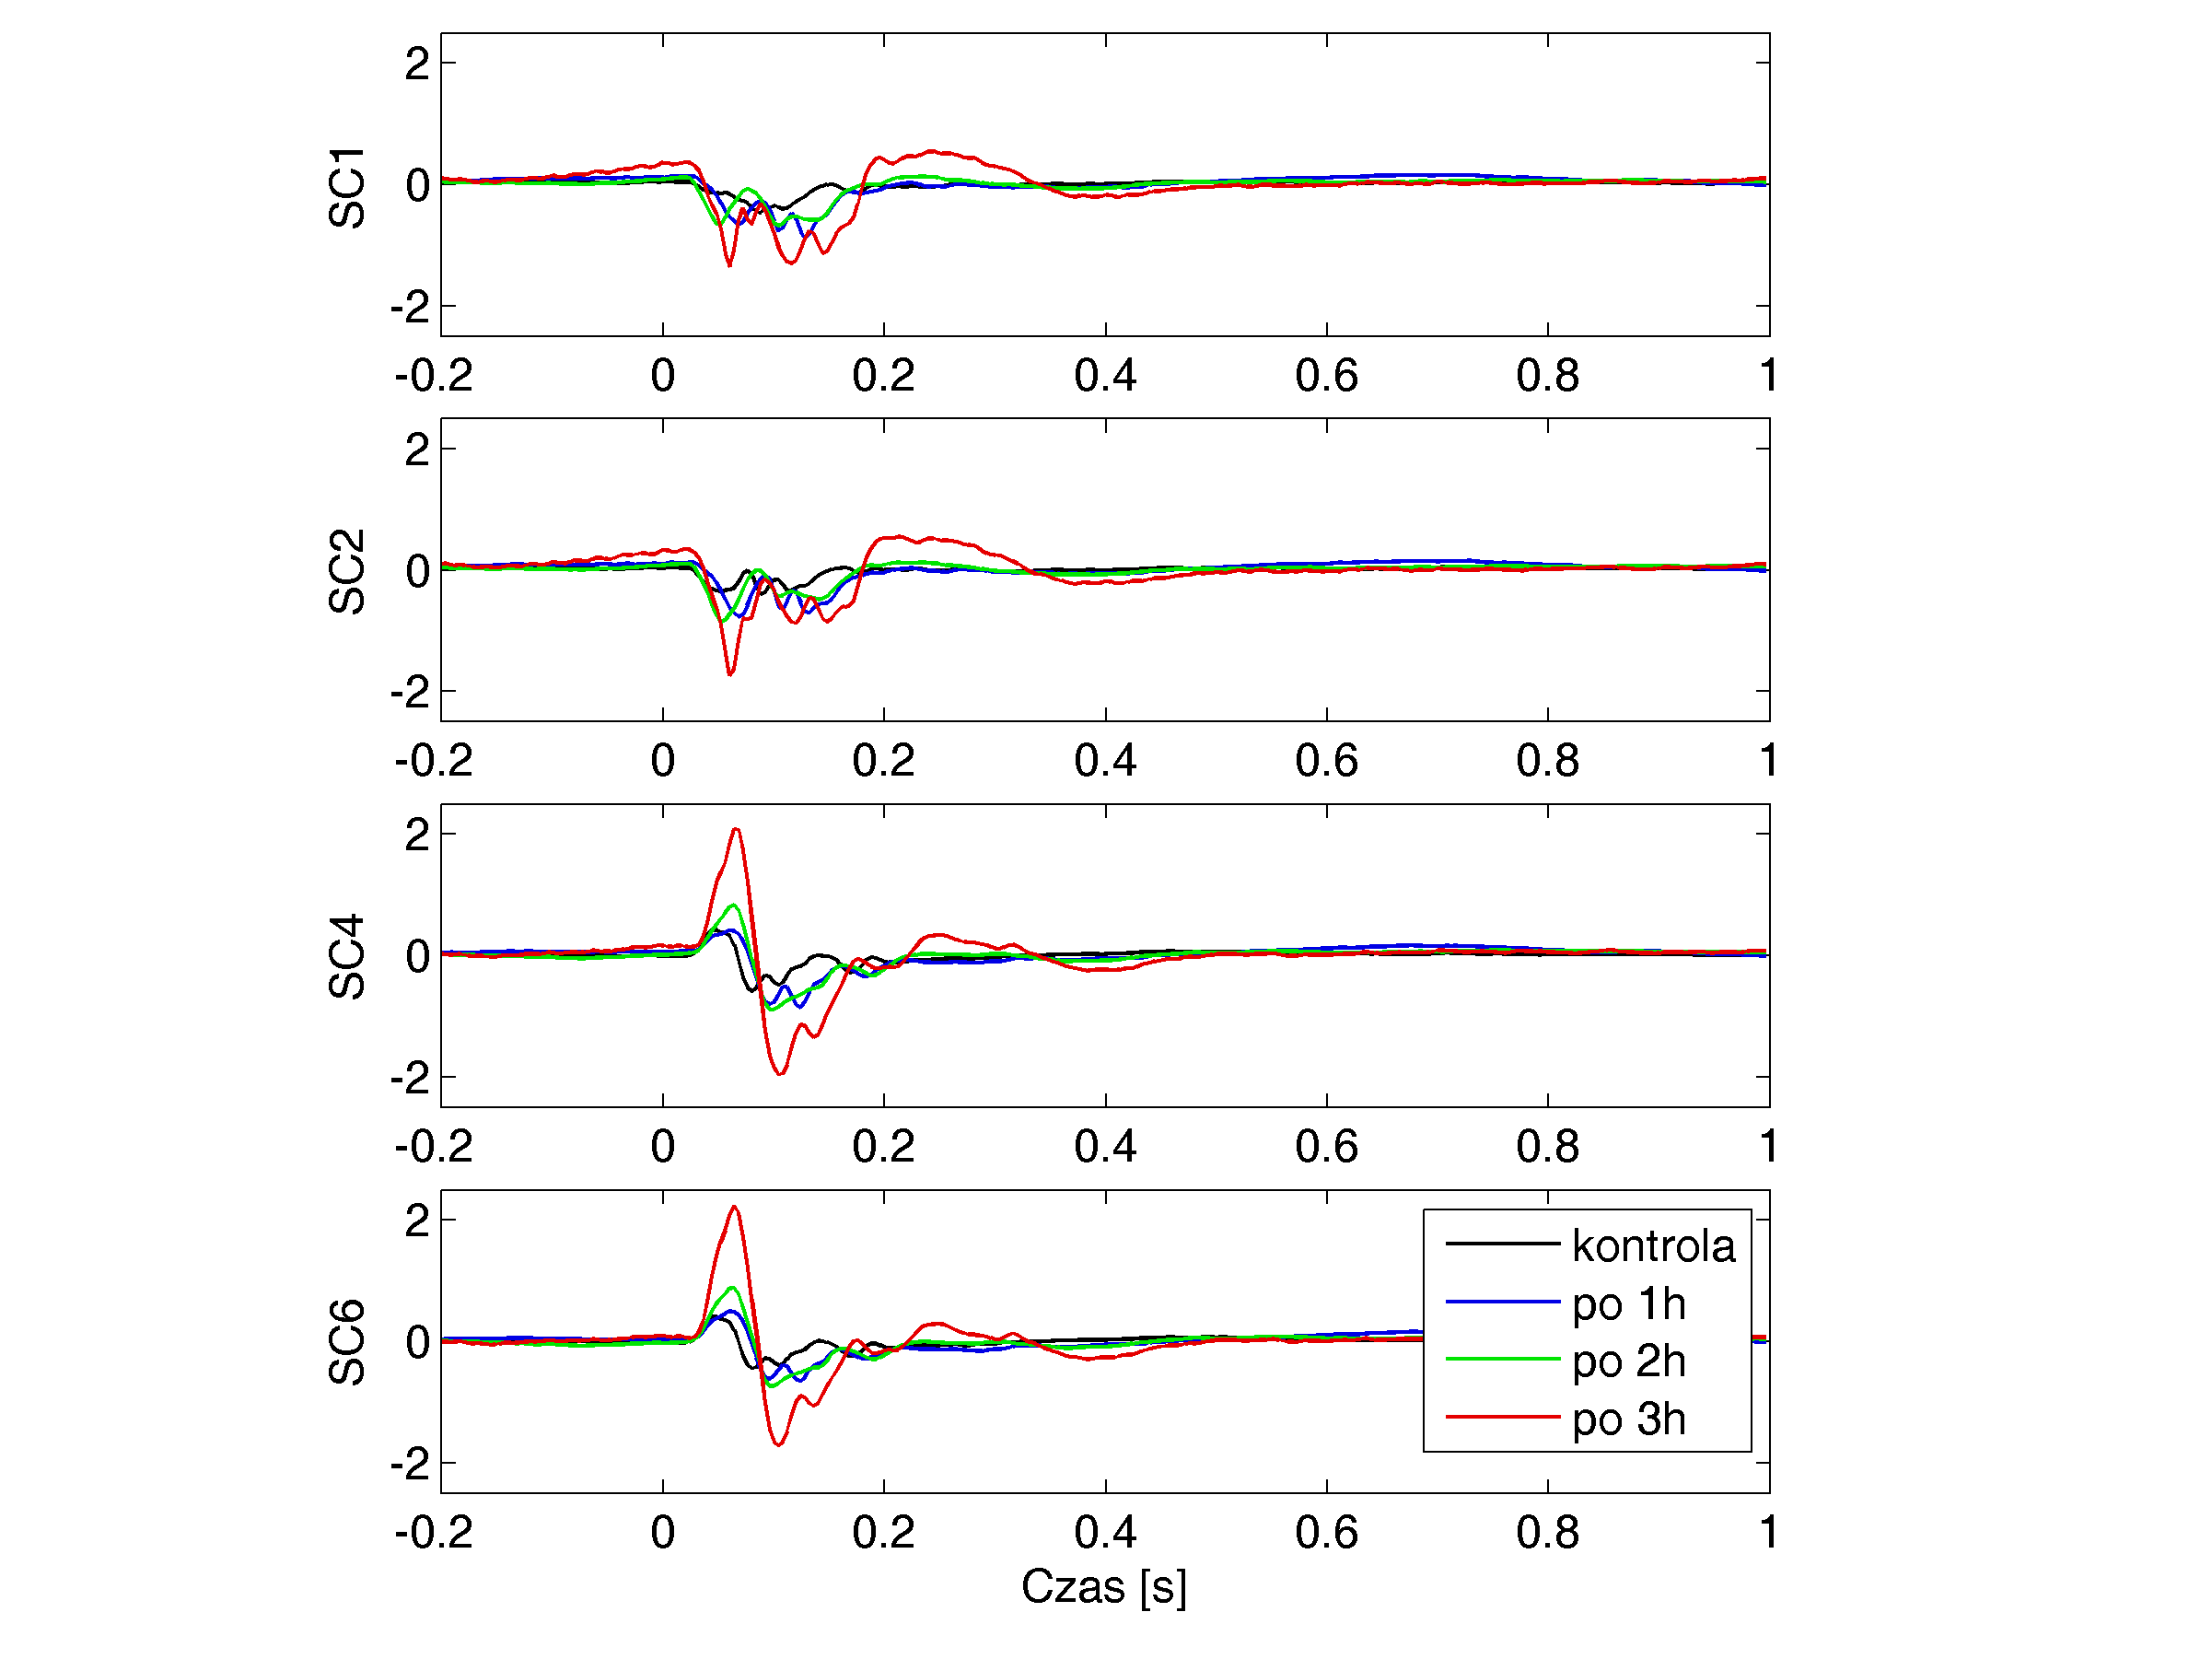
\includegraphics[scale=0.8]{kontrola15_SC.png}
		\end{center}
		\caption{Eksperyment A: Uśrednione po realizacjach potencjały wywołane. Kolorami zaznaczono kolejne godziny treningu.}
		\label{rys:kontrola15_SC}
	\end{figure}
	\begin{figure}[htbp]
		\begin{center}
			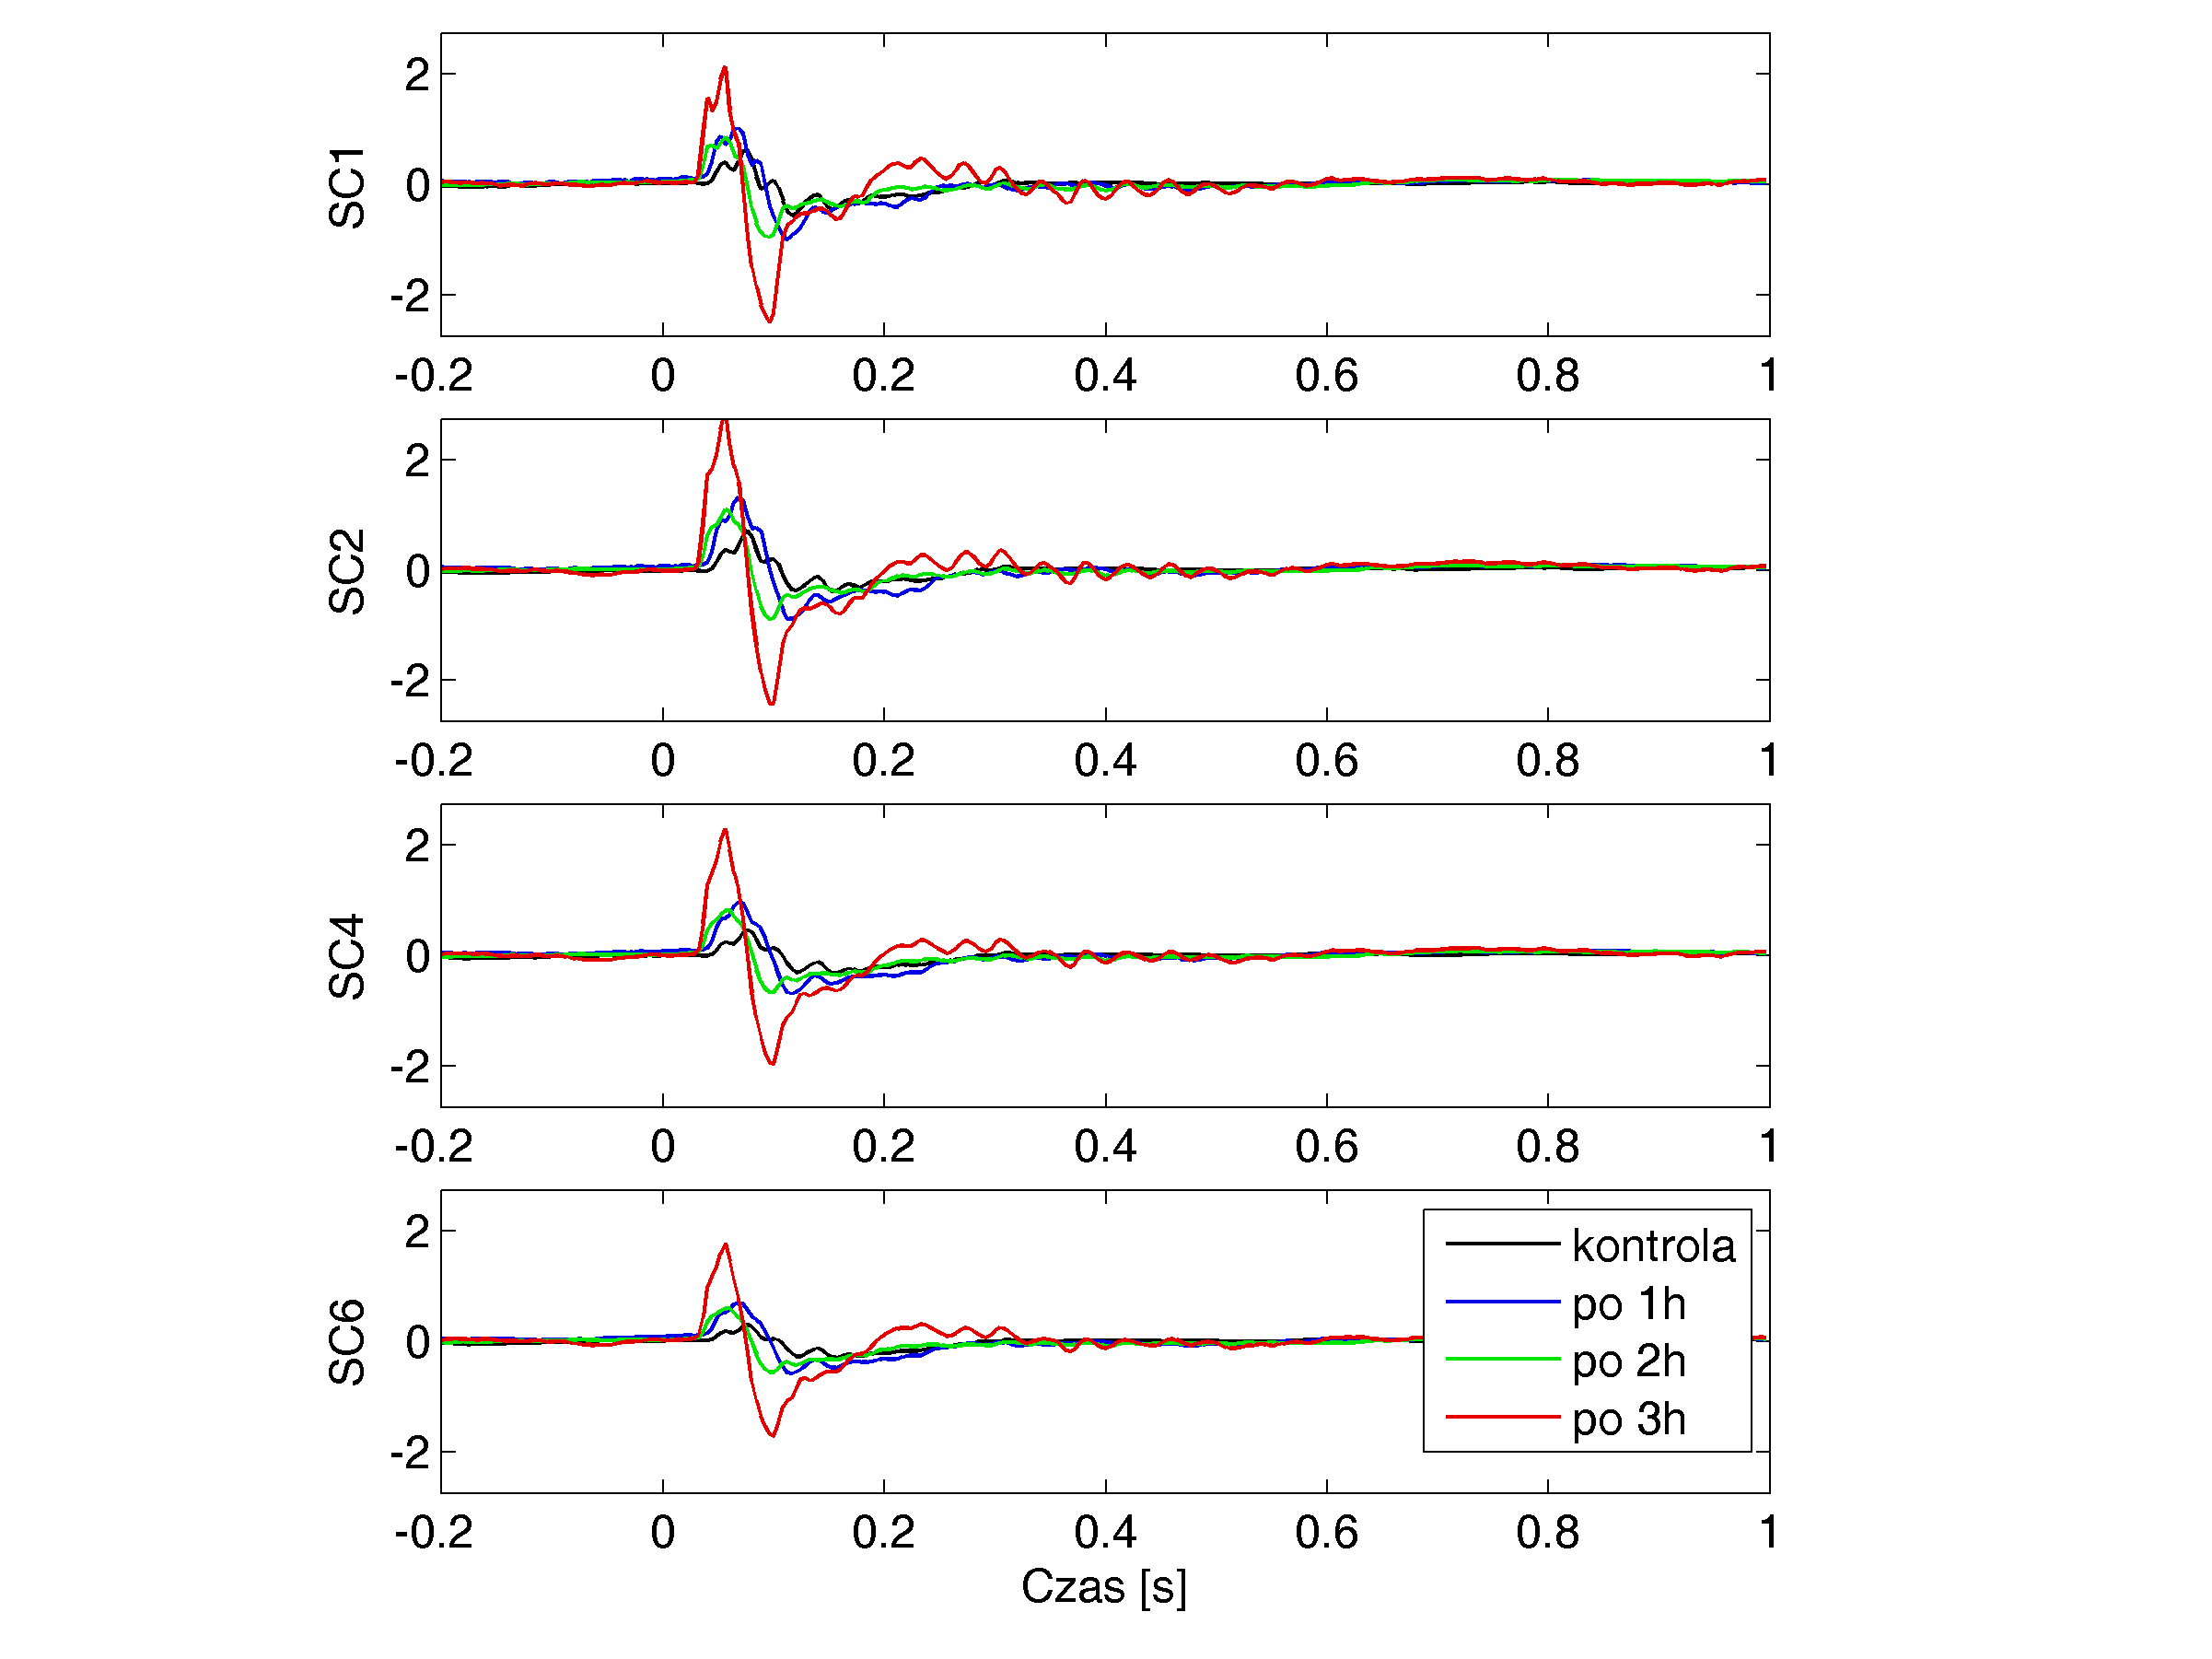
\includegraphics[scale=0.8]{beta3_SC.png}
		\end{center}
		\caption{Eksperyment B: Uśrednione po realizacjach potencjały wywołane. Kolorami zaznaczono kolejne godziny treningu.}
		\label{rys:beta3_SC}
	\end{figure}
	\FloatBarrier
	W Tabelach \ref{tab:kontrola_SC_P} i \ref{tab:beta_SC_P} zamieszono wartości statystyki dla obu zestawów danych. W obu przypadkach widoczny jest istotny wzrost amplitudy.
	\begin{table}[htdp]
		\caption{P wartości dla SC z eksperymentu A.}
		\begin{center}
			\begin{tabularx}{0.9\textwidth}{l C C C C}
				\toprule
				\textbf{} & \textbf{SC1} & \textbf{SC2} & \textbf{SC4} & \textbf{SC6} \\
				\midrule
				kontrola vs po 1 h & 0,001 & 0,001 & 0,03  & 0,007\\
				kontrola vs po 2 h & 0,001 & 0,001 & 0,001 & 0,001\\
				kontrola vs po 3 h & 0,001 & 0,001 & 0,001 & 0,001\\
				\bottomrule
			\end{tabularx}
		\end{center}
		\label{tab:kontrola_SC_P}
	\end{table}
	\begin{table}[htdp]
		\caption{P wartości dla SC z eksperymentu B.}
		\begin{center}
			\begin{tabularx}{0.9\textwidth}{l C C C C}
				\toprule
				\textbf{} & \textbf{SC1} & \textbf{SC2} & \textbf{SC4} & \textbf{SC6} \\
				\midrule
				kontrola vs po 1 h & 0,001 & 0,001 & 0,007  & 0,002\\
				kontrola vs po 2 h & 0,001 & 0,001 & 0,001 & 0,001\\
				kontrola vs po 3 h & 0,001 & 0,001 & 0,001 & 0,001\\
				\bottomrule
			\end{tabularx}
		\end{center}
		\label{tab:beta_SC_P}
	\end{table}
	\FloatBarrier
	\subsection{Porównanie uśrednionych potencjałów z LGN}
	W przypadku jądra kolankowatego bocznego (LGN) dla obu eksperymentów wybrano kanał, który charakteryzował się najwyższą amplitudą (Rysunek \ref{rys:porownanie_LGN}).
	\begin{figure}[h]
		\begin{center}
			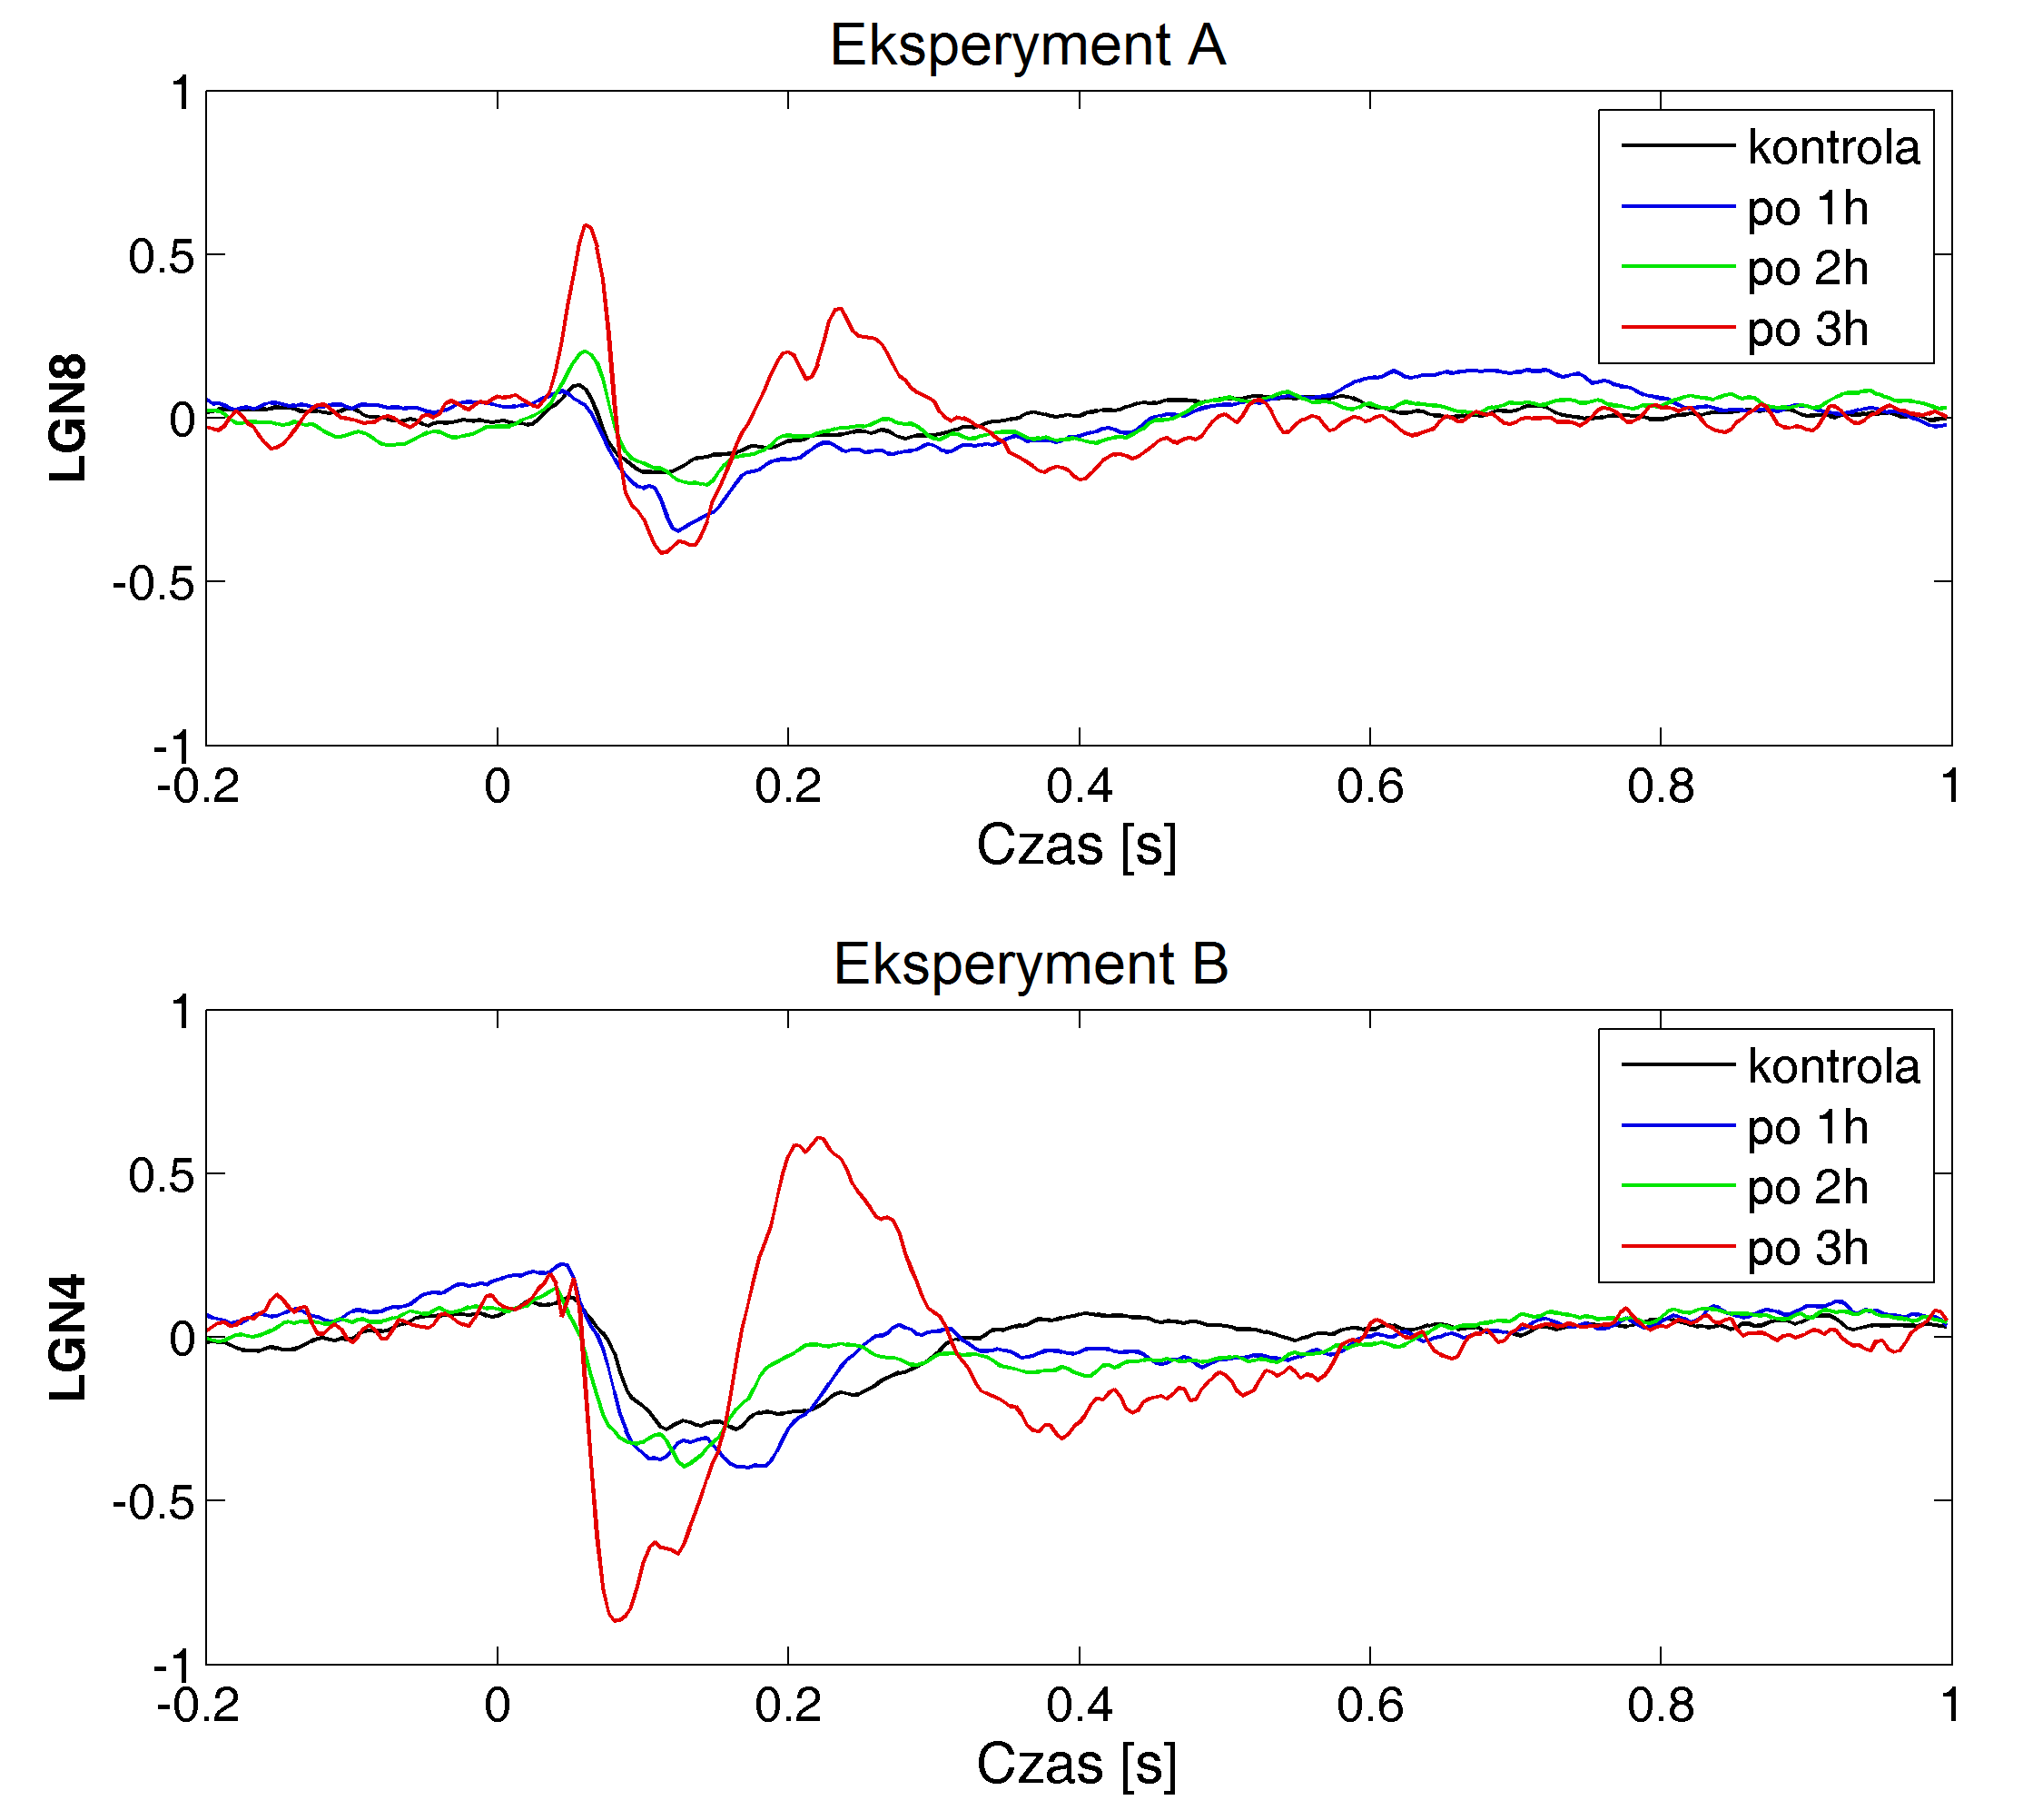
\includegraphics[width=0.7\columnwidth]{porownanie_LGN.png}
		\end{center}
		\caption{Porównanie uśrednionych potencjałów z LGN.}
		\label{rys:porownanie_LGN}
	\end{figure}
	\FloatBarrier
	W Tabeli \ref{tab:oba_LGN_P} przedstawiono wartości p testu statystycznego. P wartości dla danych z eksperymentu B są dużo niższe niż dla danych z eksperymentu A, co może świadczyć o wpływie stymulacji elektrycznej na zwiększenie amplitudy potencjału wywołanego.
	\begin{table}[htdp]
		\caption{P wartości dla LGN z eksperymentu A i B.}
		\begin{center}
			\begin{tabularx}{0.5\textwidth}{l C C}
				\toprule
				\textbf{} & \textbf{A: CxC8} & \textbf{B: CxC4}\\
				\midrule
				kontrola vs po 1 h & 0,201 & 0,001\\
				kontrola vs po 2 h & 0,030 & 0,003\\
				kontrola vs po 3 h & 0,001 & 0,001\\
				\bottomrule
			\end{tabularx}
		\end{center}
		\label{tab:oba_LGN_P}
	\end{table}
	
	\section{Połączenia funkcjonalne}
	W analizie połączeń funkcjonalnych pominięto analizę CxI ze względu na to, że w danych z eksperymentu A pojawiły się artefakty, a dla danych z eksperymentu B potencjały wywołane miały nietypowy przebieg w czasie (Sekcja \ref{CxI}).
	
	Statystykę przeprowadzono zgodnie z opisem zawartym w Sekcji \ref{NDTF}. Niebieskim kolorem zaznaczono 95\%-owe przedziały ufności, w których znajdują się wartości funkcji NDTF danych kontrolnych, a czerwonym przedziały wartości dla kolejnych godzin treningu. Dodatkowo, krzywą w korespondującym kolorze zaznaczono średnie wartości funkcji NDTF dla danego zakresu częstości.	
	Za istotnie różne można uznać te przedziały, które nie pokrywają się z danymi kontrolnymi. Litery A, B i C odpowiadają porównaniom między danymi kontrolnymi a odpowiednio: pierwszą, drugą i trzecią godziną treningu.
	
	%Do analizy połączeń SC wykorzystano tylko dwa głębsze kanały (SC4 i SC6), ponieważ prawdopodobnie nie udało się zarejestrować potencjału z płytszych warstw dla danych z eksperymentu B (Sekcja \ref{SC}).
	\subsection{Połączenia z CxC do LGN}
	Do analizy wykorzystano kanały: z zestawu A: CxC8 i LGN8 oraz z zestawu B: CxC5 i LGN4.
	Na Rysunkach \ref{rys:1_10_CxC_LGN}, \ref{rys:10_30_CxC_LGN} i \ref{rys:20_40_CxC_LGN} przedstawiono wartości funkcji NDTF dla kolejnych zakresów częstości. Dla częstości 1-10 Hz dla danych z eksperymentu A (Rysunek \ref{rys:1_10_kon_CxC_LGN}) wartości funkcji NDTF po kolejnych godzinach treningu nie przekraczają wartości kontrolnych. Natomiast dla danych z eksperymentu B (Rysunek \ref{rys:1_10_beta_CxC_LGN}) występuje  nieznaczny pik zaraz po podaniu bodźca (czas 0-0,1 s) oraz wysoki pik około 0,2 s po 3 godzinach treningu wzrokowego. 
		\begin{figure}[h]
		\begin{subfigure}{.5\textwidth}
			\centering
			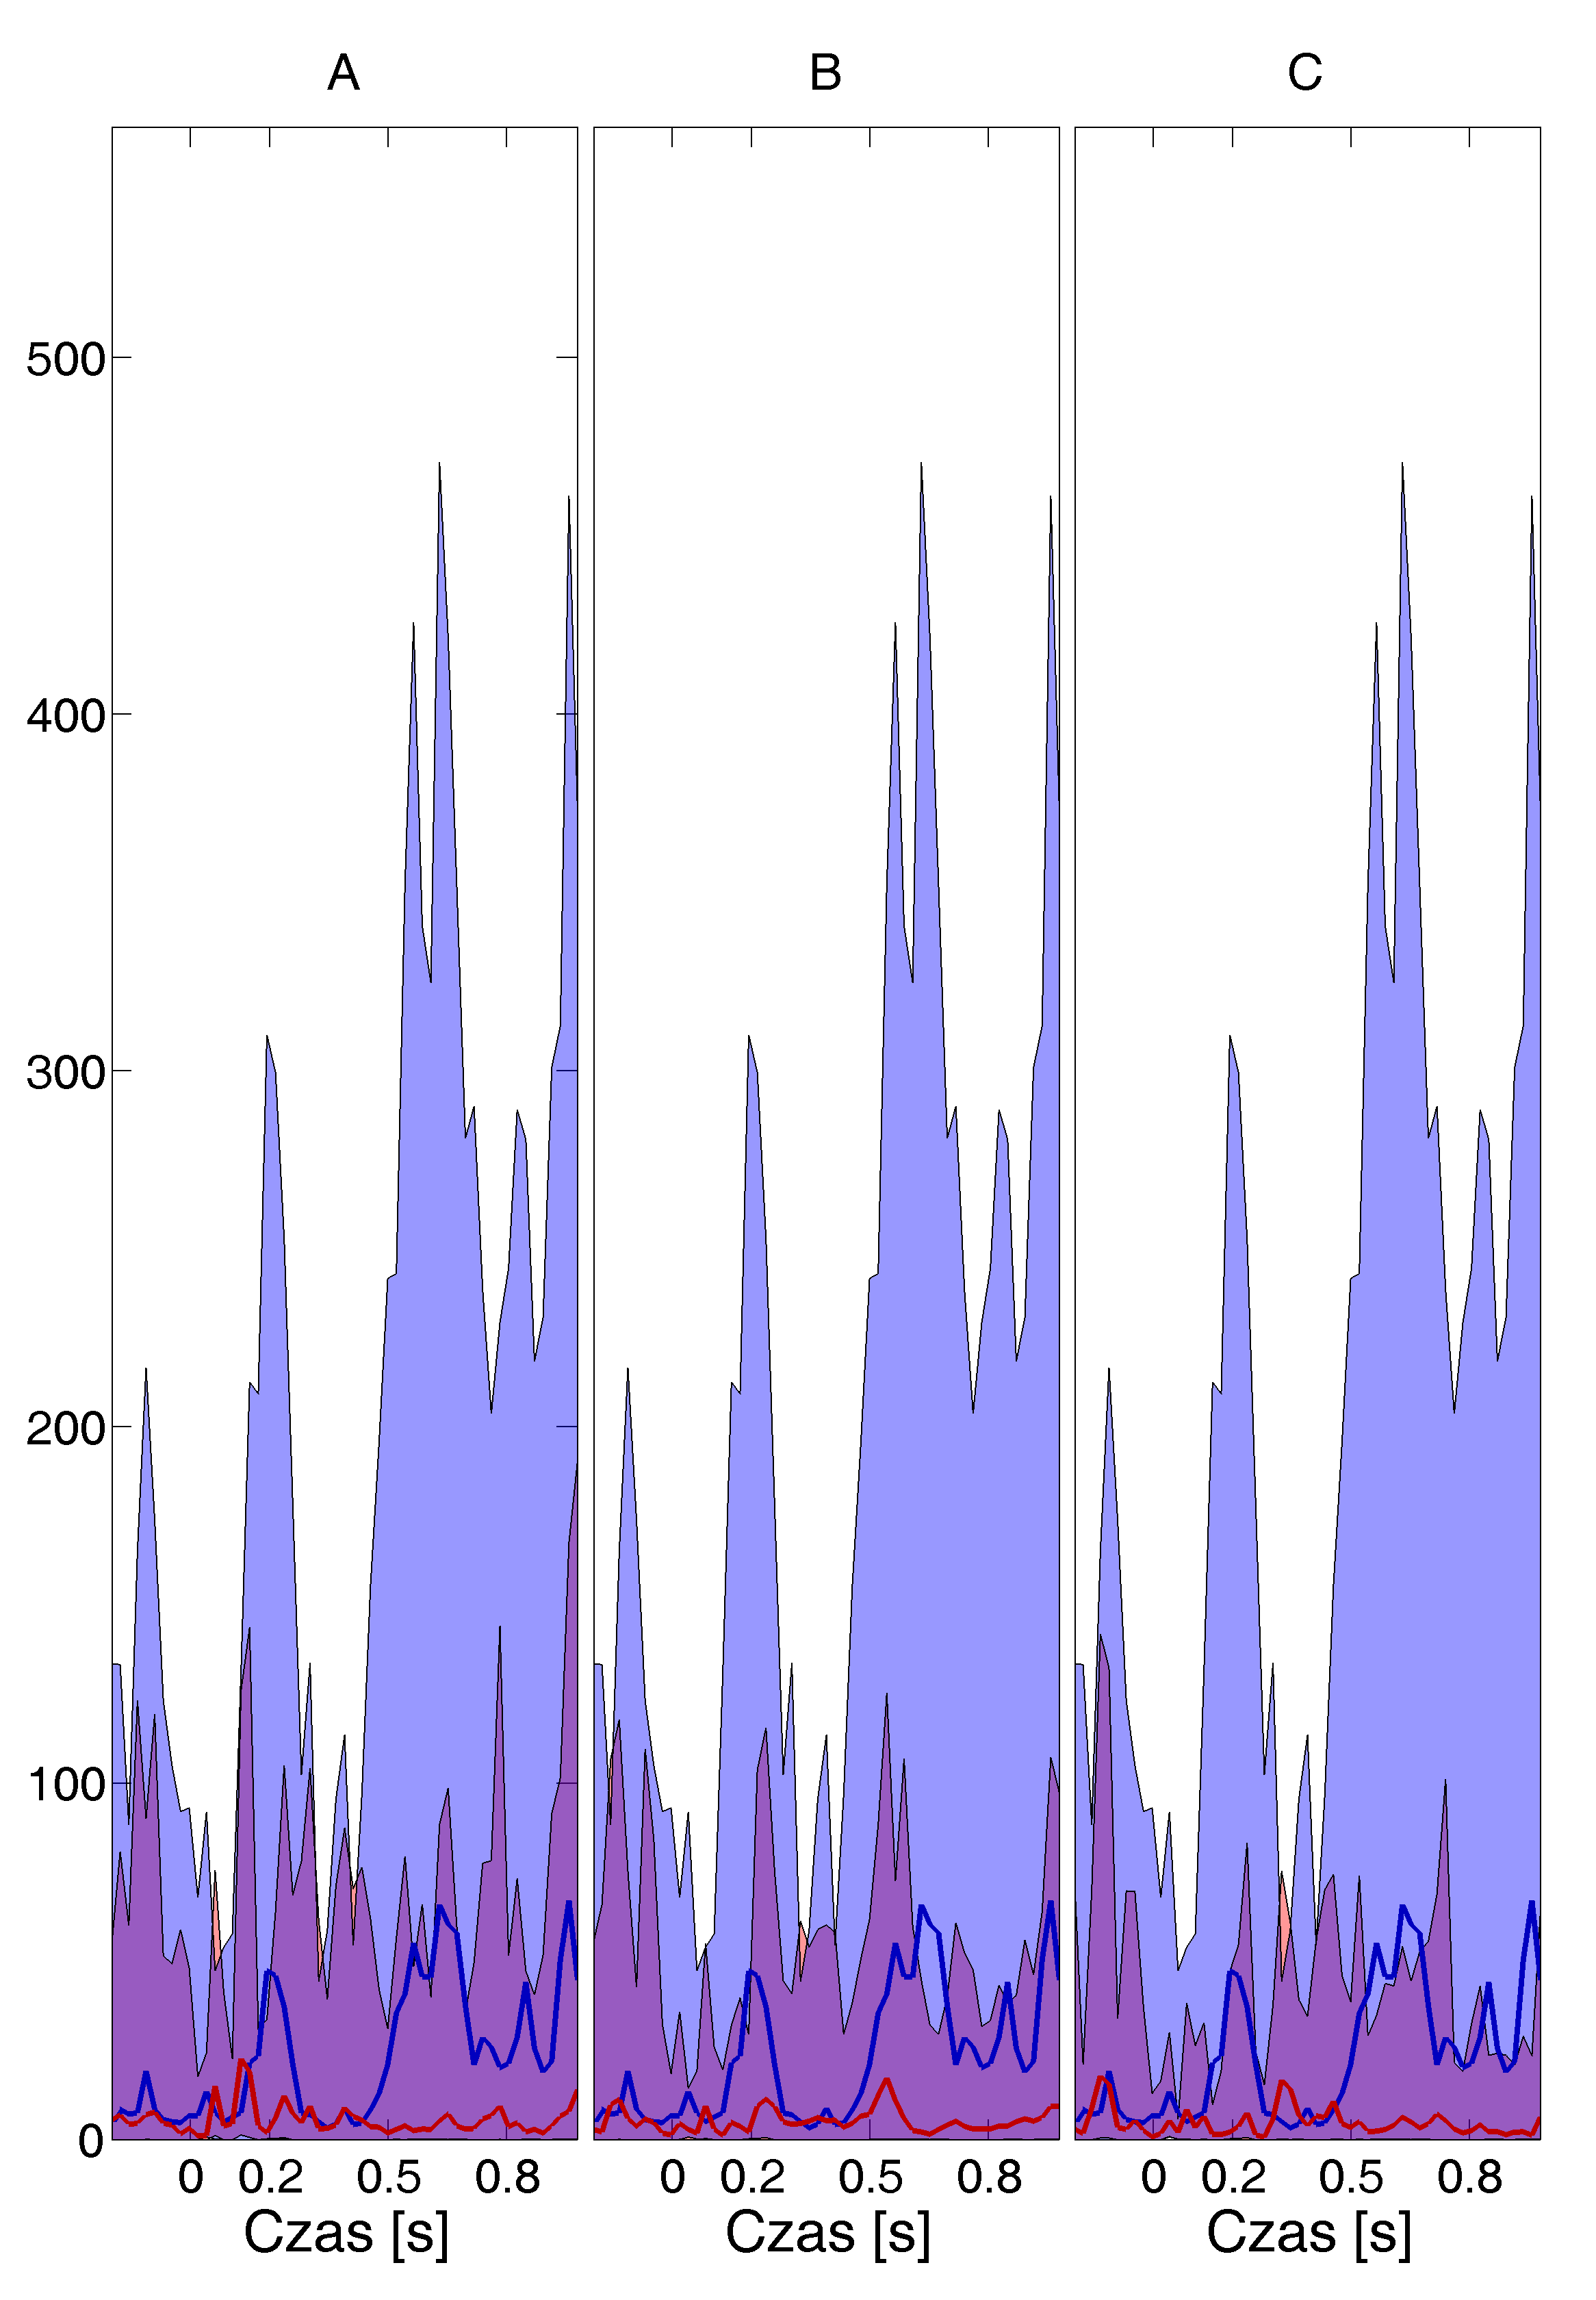
\includegraphics[width=1.\linewidth]{kontrola15_1-10_z_CxC8_do_LGN82.png}
			\caption{Bez stymulacji elektrycznej}
			\label{rys:1_10_kon_CxC_LGN}
		\end{subfigure}%
		\begin{subfigure}{.5\textwidth}
			\centering
			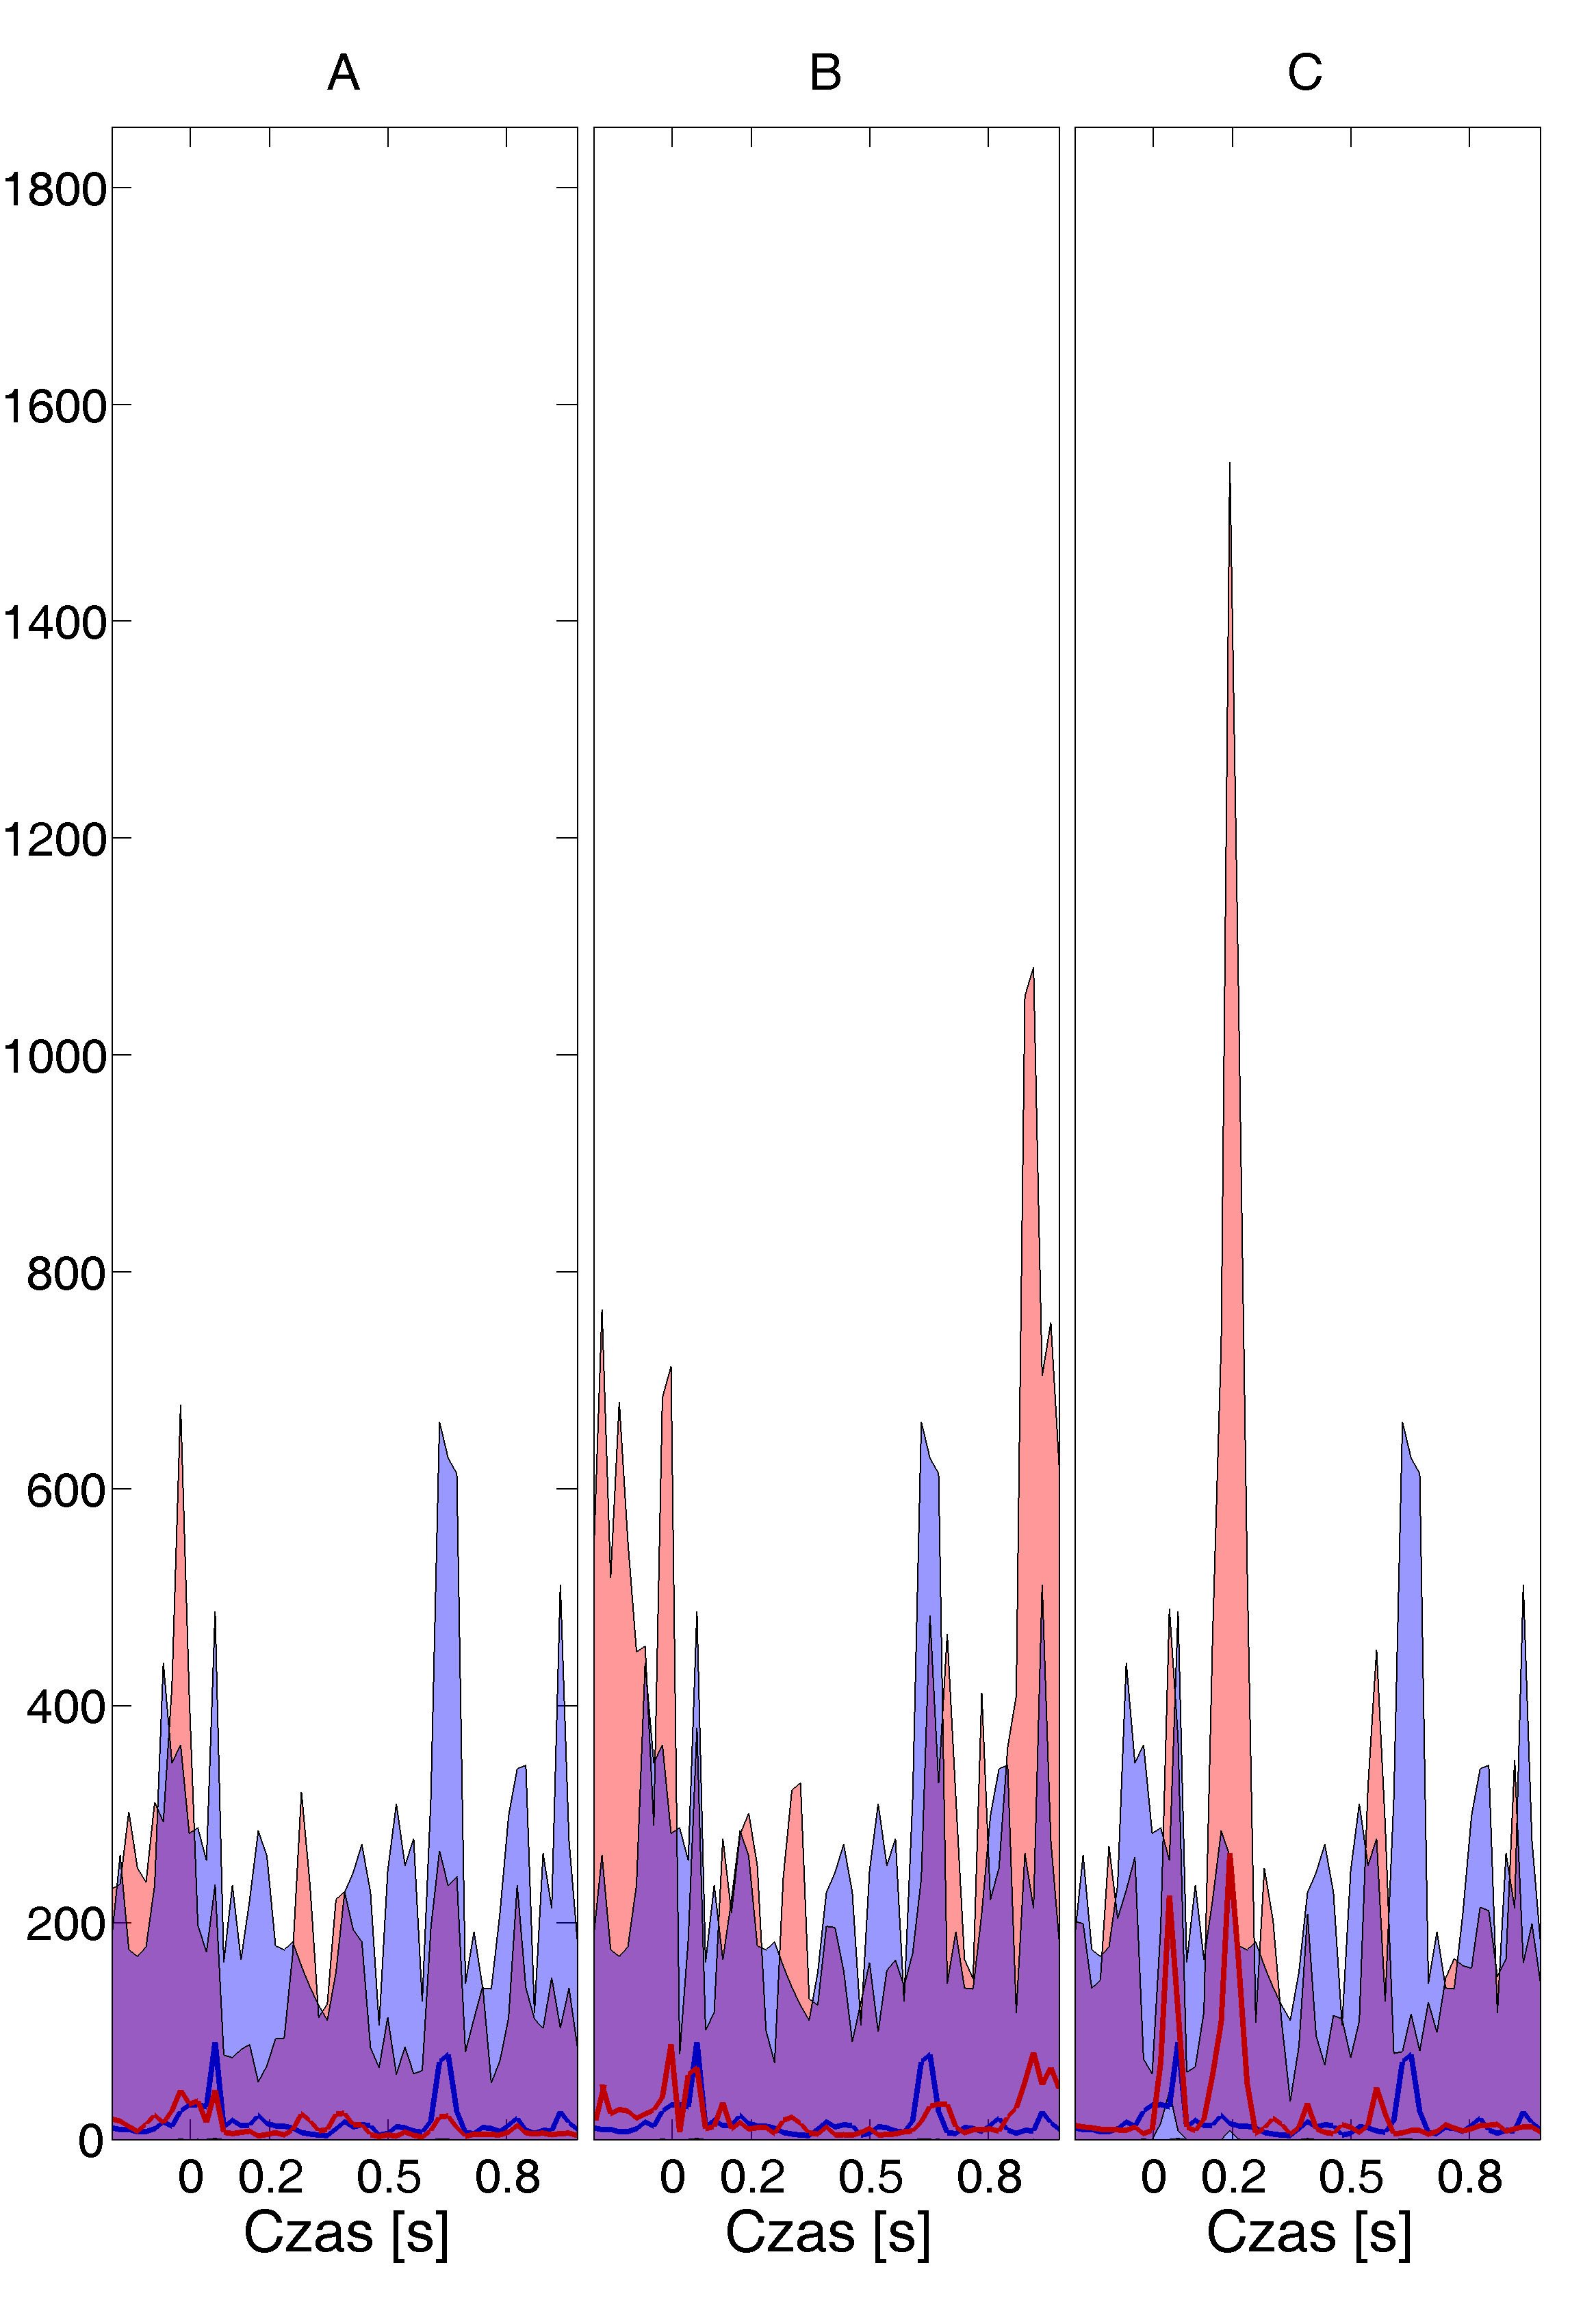
\includegraphics[width=1.\linewidth]{beta3_1-10_z_CxC5_do_LGN42.png}
			\caption{Po stymulacji elektrycznej}
			\label{rys:1_10_beta_CxC_LGN}
		\end{subfigure}
		\caption{Przedstawienie danych z różnych eksperymentów w paśmie 1-10 Hz.}
		\label{rys:1_10_CxC_LGN}
	\end{figure}
	\FloatBarrier
	Dla zakresu częstości 10-30 Hz dla danych z eksperymentu A (Rysunek \ref{rys:10_30_kon_CxC_LGN}) można zauważyć niewielki pik w 0-0,1 s po pierwszej i trzeciej godzinie treningu. Dla eksperymentu B (Rysunek \ref{rys:10_30_beta_CxC_LGN}) różnica wartości funkcji NDTF między danymi kontrolnymi a danymi z kolejnych godzin treningu w czasie 0-0,1 s jest większa niż dla danych z eksperymentu A. Ponadto po trzeciej godzinie treningu pojawia się pik w 0,2 s.
	%Podobne obserwacje można poczynić dla zakresu częstości 10-30 Hz i 20-40 Hz. W obu przypadkach, dla danych z eksperymentu A (Rysunki \ref{rys:10_30_kon_CxC_LGN} i \ref{rys:20_40_kon_CxC_LGN}) wartości funkcji NDTF dla danych po kolejnych godzinach treningu niewiele różnią się od danych kontrolnych, natomiast po stymulacji elektrycznej (Rysunki \ref{rys:10_30_beta_CxC_LGN} i \ref{rys:20_40_beta_CxC_LGN}) widoczne są wyraźne piki w przedziale 0-0,1 s i w 0,2 s po wystąpieniu bodźca. 
	\begin{figure}[h]
		\begin{subfigure}{.5\textwidth}
			\centering
			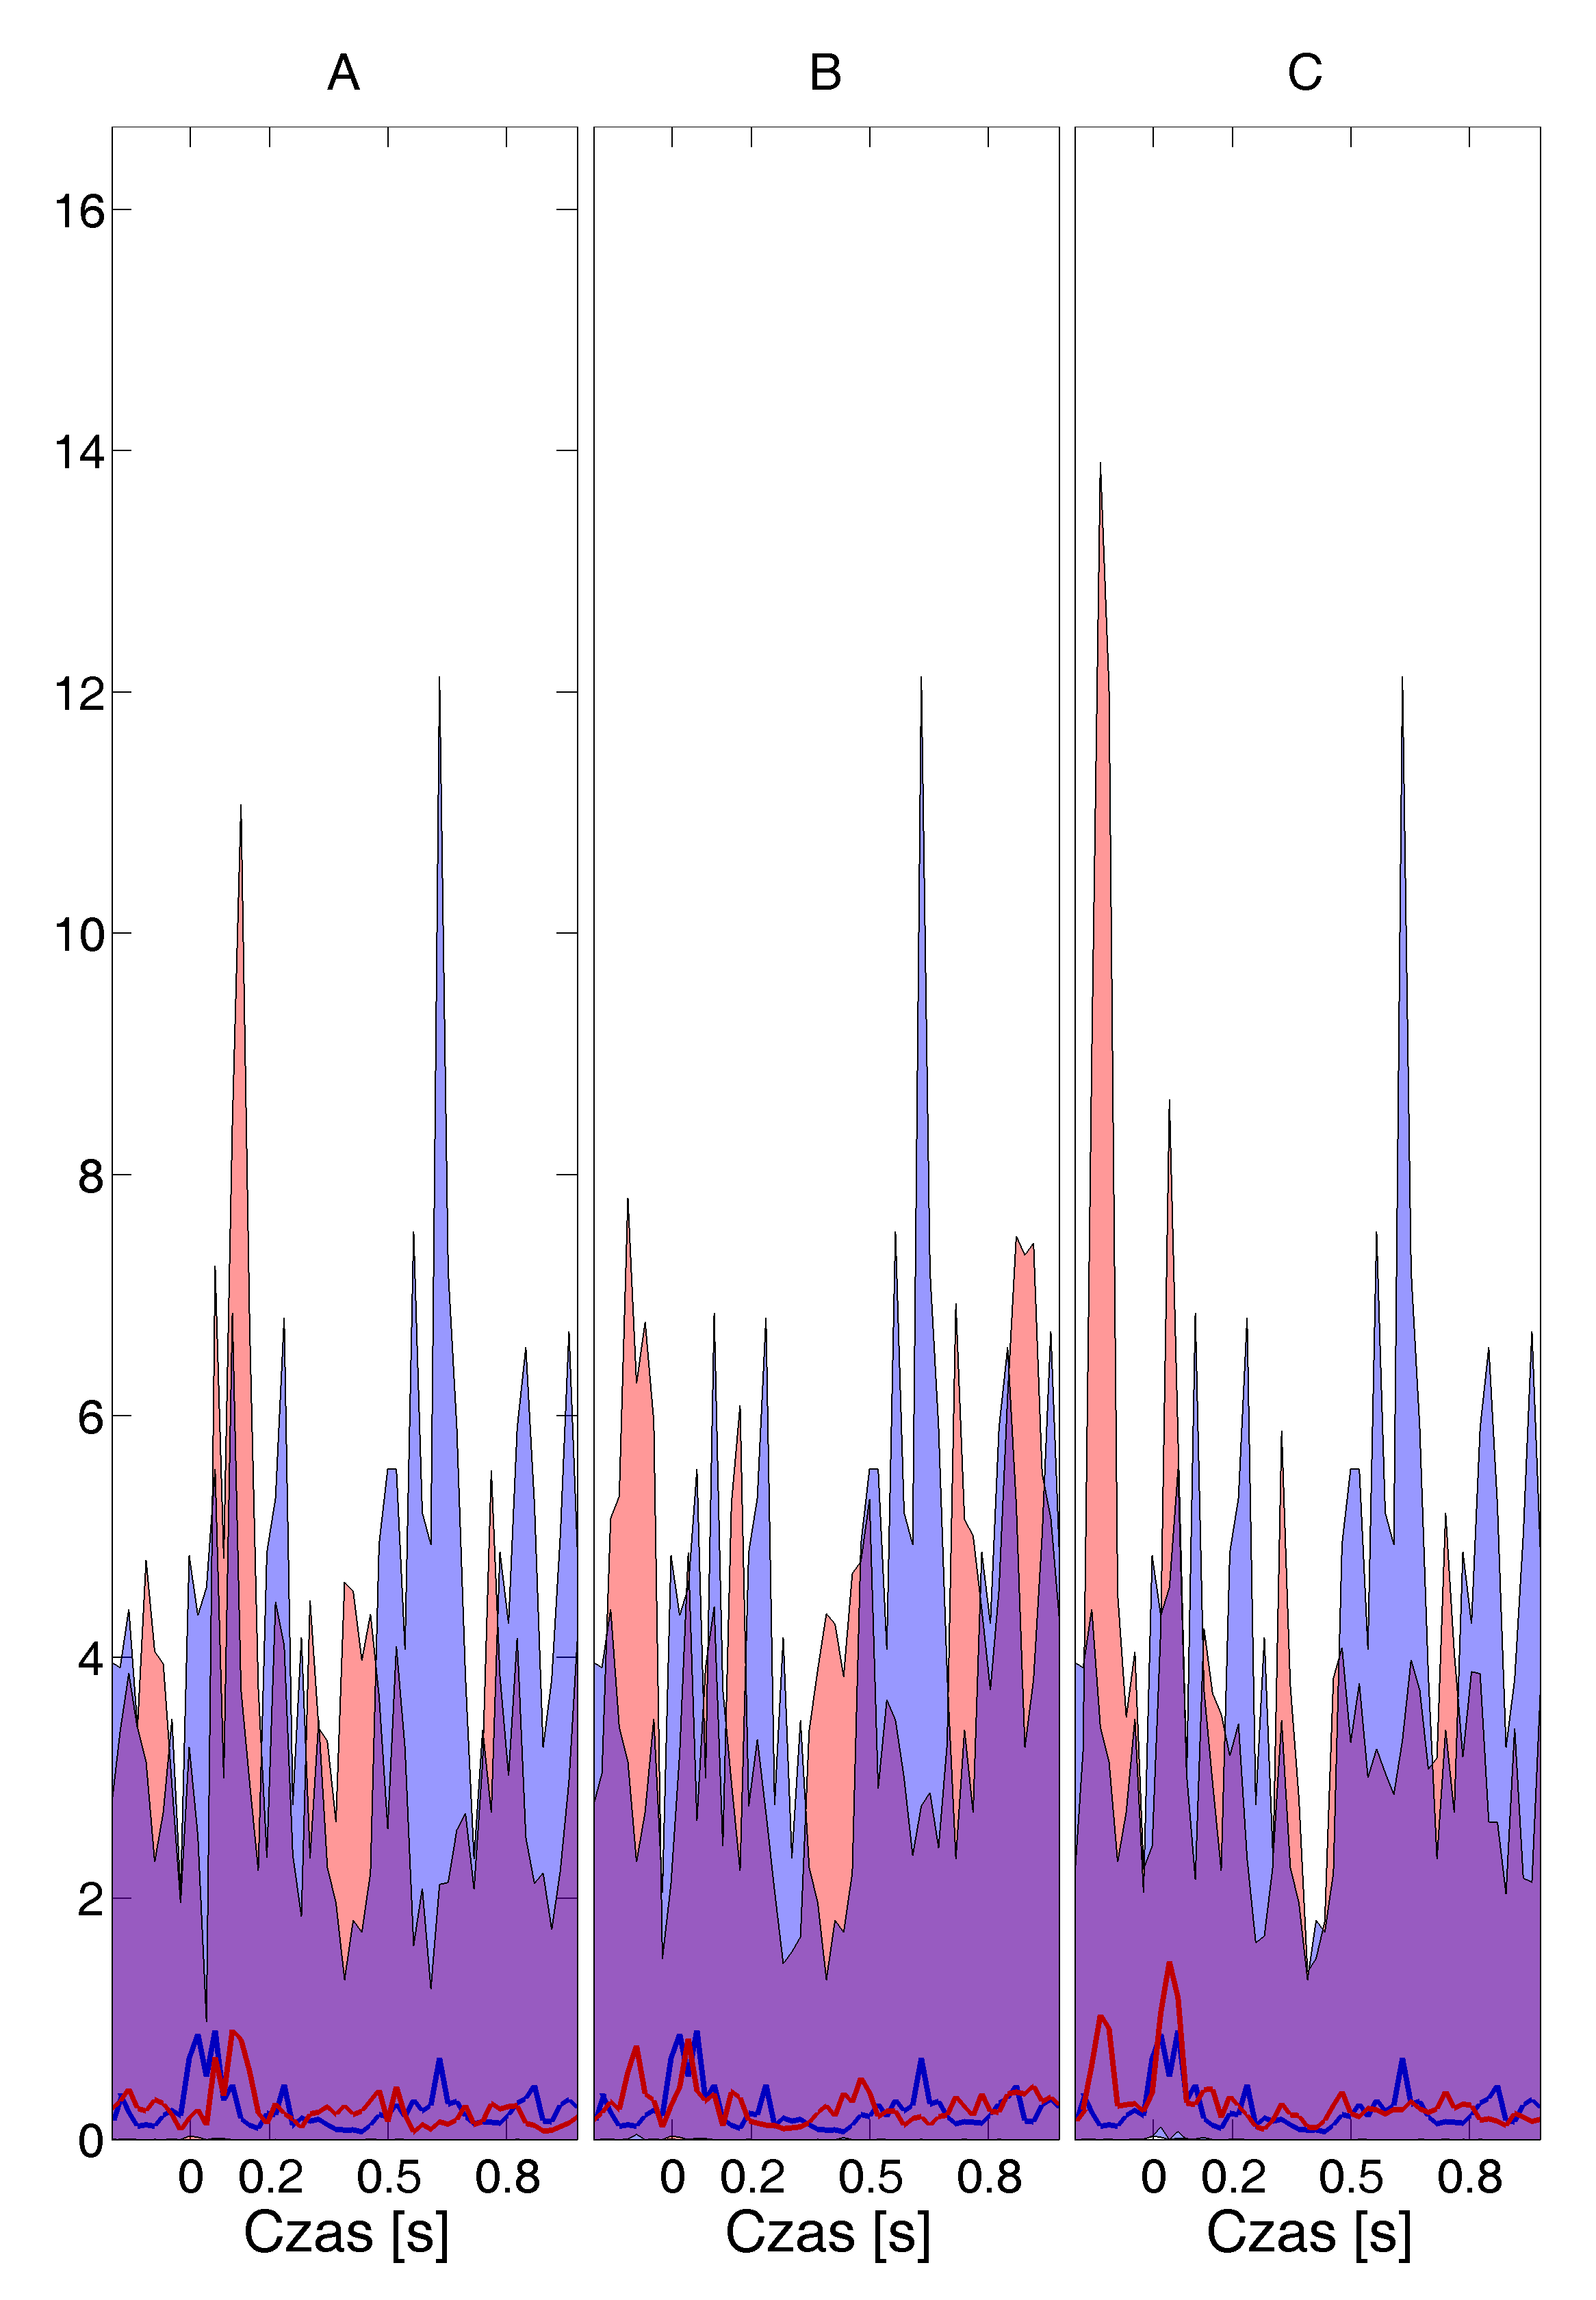
\includegraphics[width=1.\linewidth]{kontrola15_10-30_z_CxC8_do_LGN82.png}
			\caption{Bez stymulacji elektrycznej}
			\label{rys:10_30_kon_CxC_LGN}
		\end{subfigure}%
		\begin{subfigure}{.5\textwidth}
			\centering
			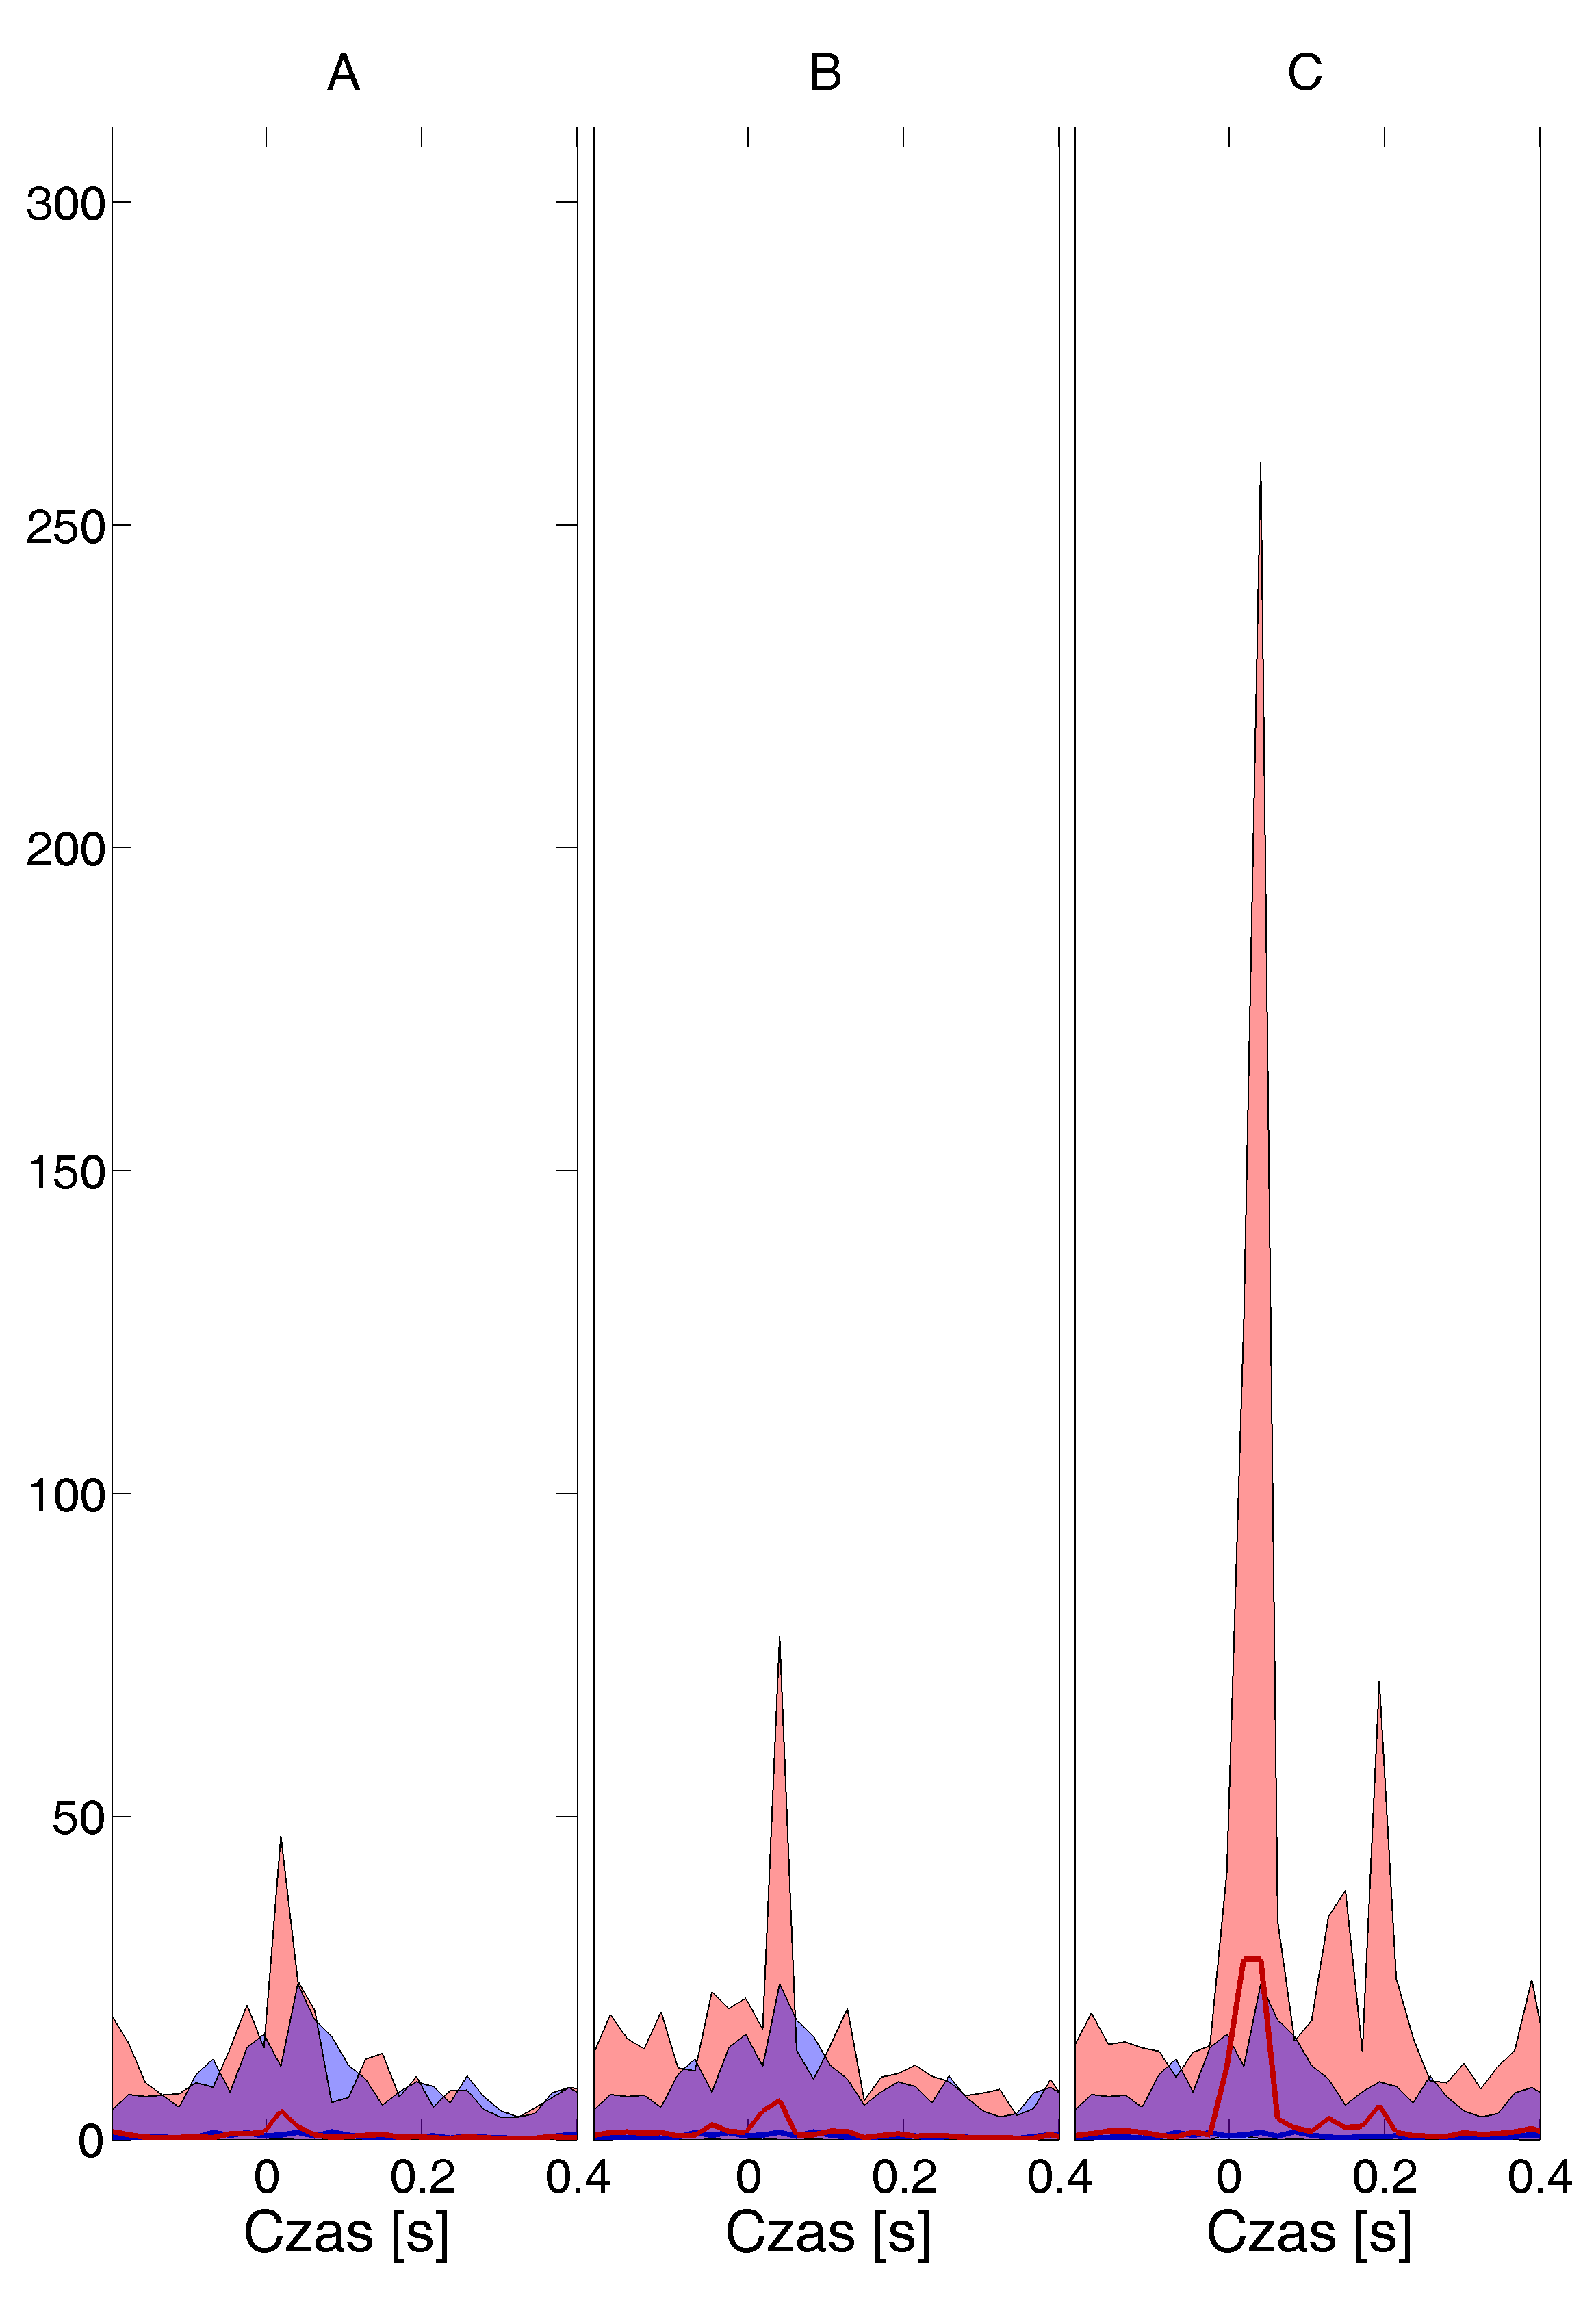
\includegraphics[width=1.\linewidth]{beta3_10-30_z_CxC5_do_LGN42.png}
			\caption{Po stymulacji elektrycznej}
			\label{rys:10_30_beta_CxC_LGN}
		\end{subfigure}
		\caption{Przedstawienie danych z różnych eksperymentów w paśmie 10-30 Hz.}
		\label{rys:10_30_CxC_LGN}
	\end{figure}
	\FloatBarrier
	Podobne obserwacje można poczynić dla zakresu częstości 20-40 Hz (Rysunek \ref{rys:20_40_CxC_LGN}). Można zauważyć, że dla obu warunków doświadczalnych na całym przedziale czasu, wartość funkcji NDTF dla kolejnych godzin treningu jest wyższa niż w danych kontrolnych. Dla danych z eksperymentu A (Rysunek \ref{rys:20_40_kon_CxC_LGN}) funkcja NDTF przyjmuje podobne wartości na całym wycinku czasowym, natomiast dla danych z eksperymentu B (Rysunek \ref{rys:20_40_beta_CxC_LGN}) widać wyraźnie pik w czasie 0-0,1 s i dla trzeciej godziny treningu -- także w 0,2 s.
	\begin{figure}[h]
		\begin{subfigure}{.5\textwidth}
			\centering
			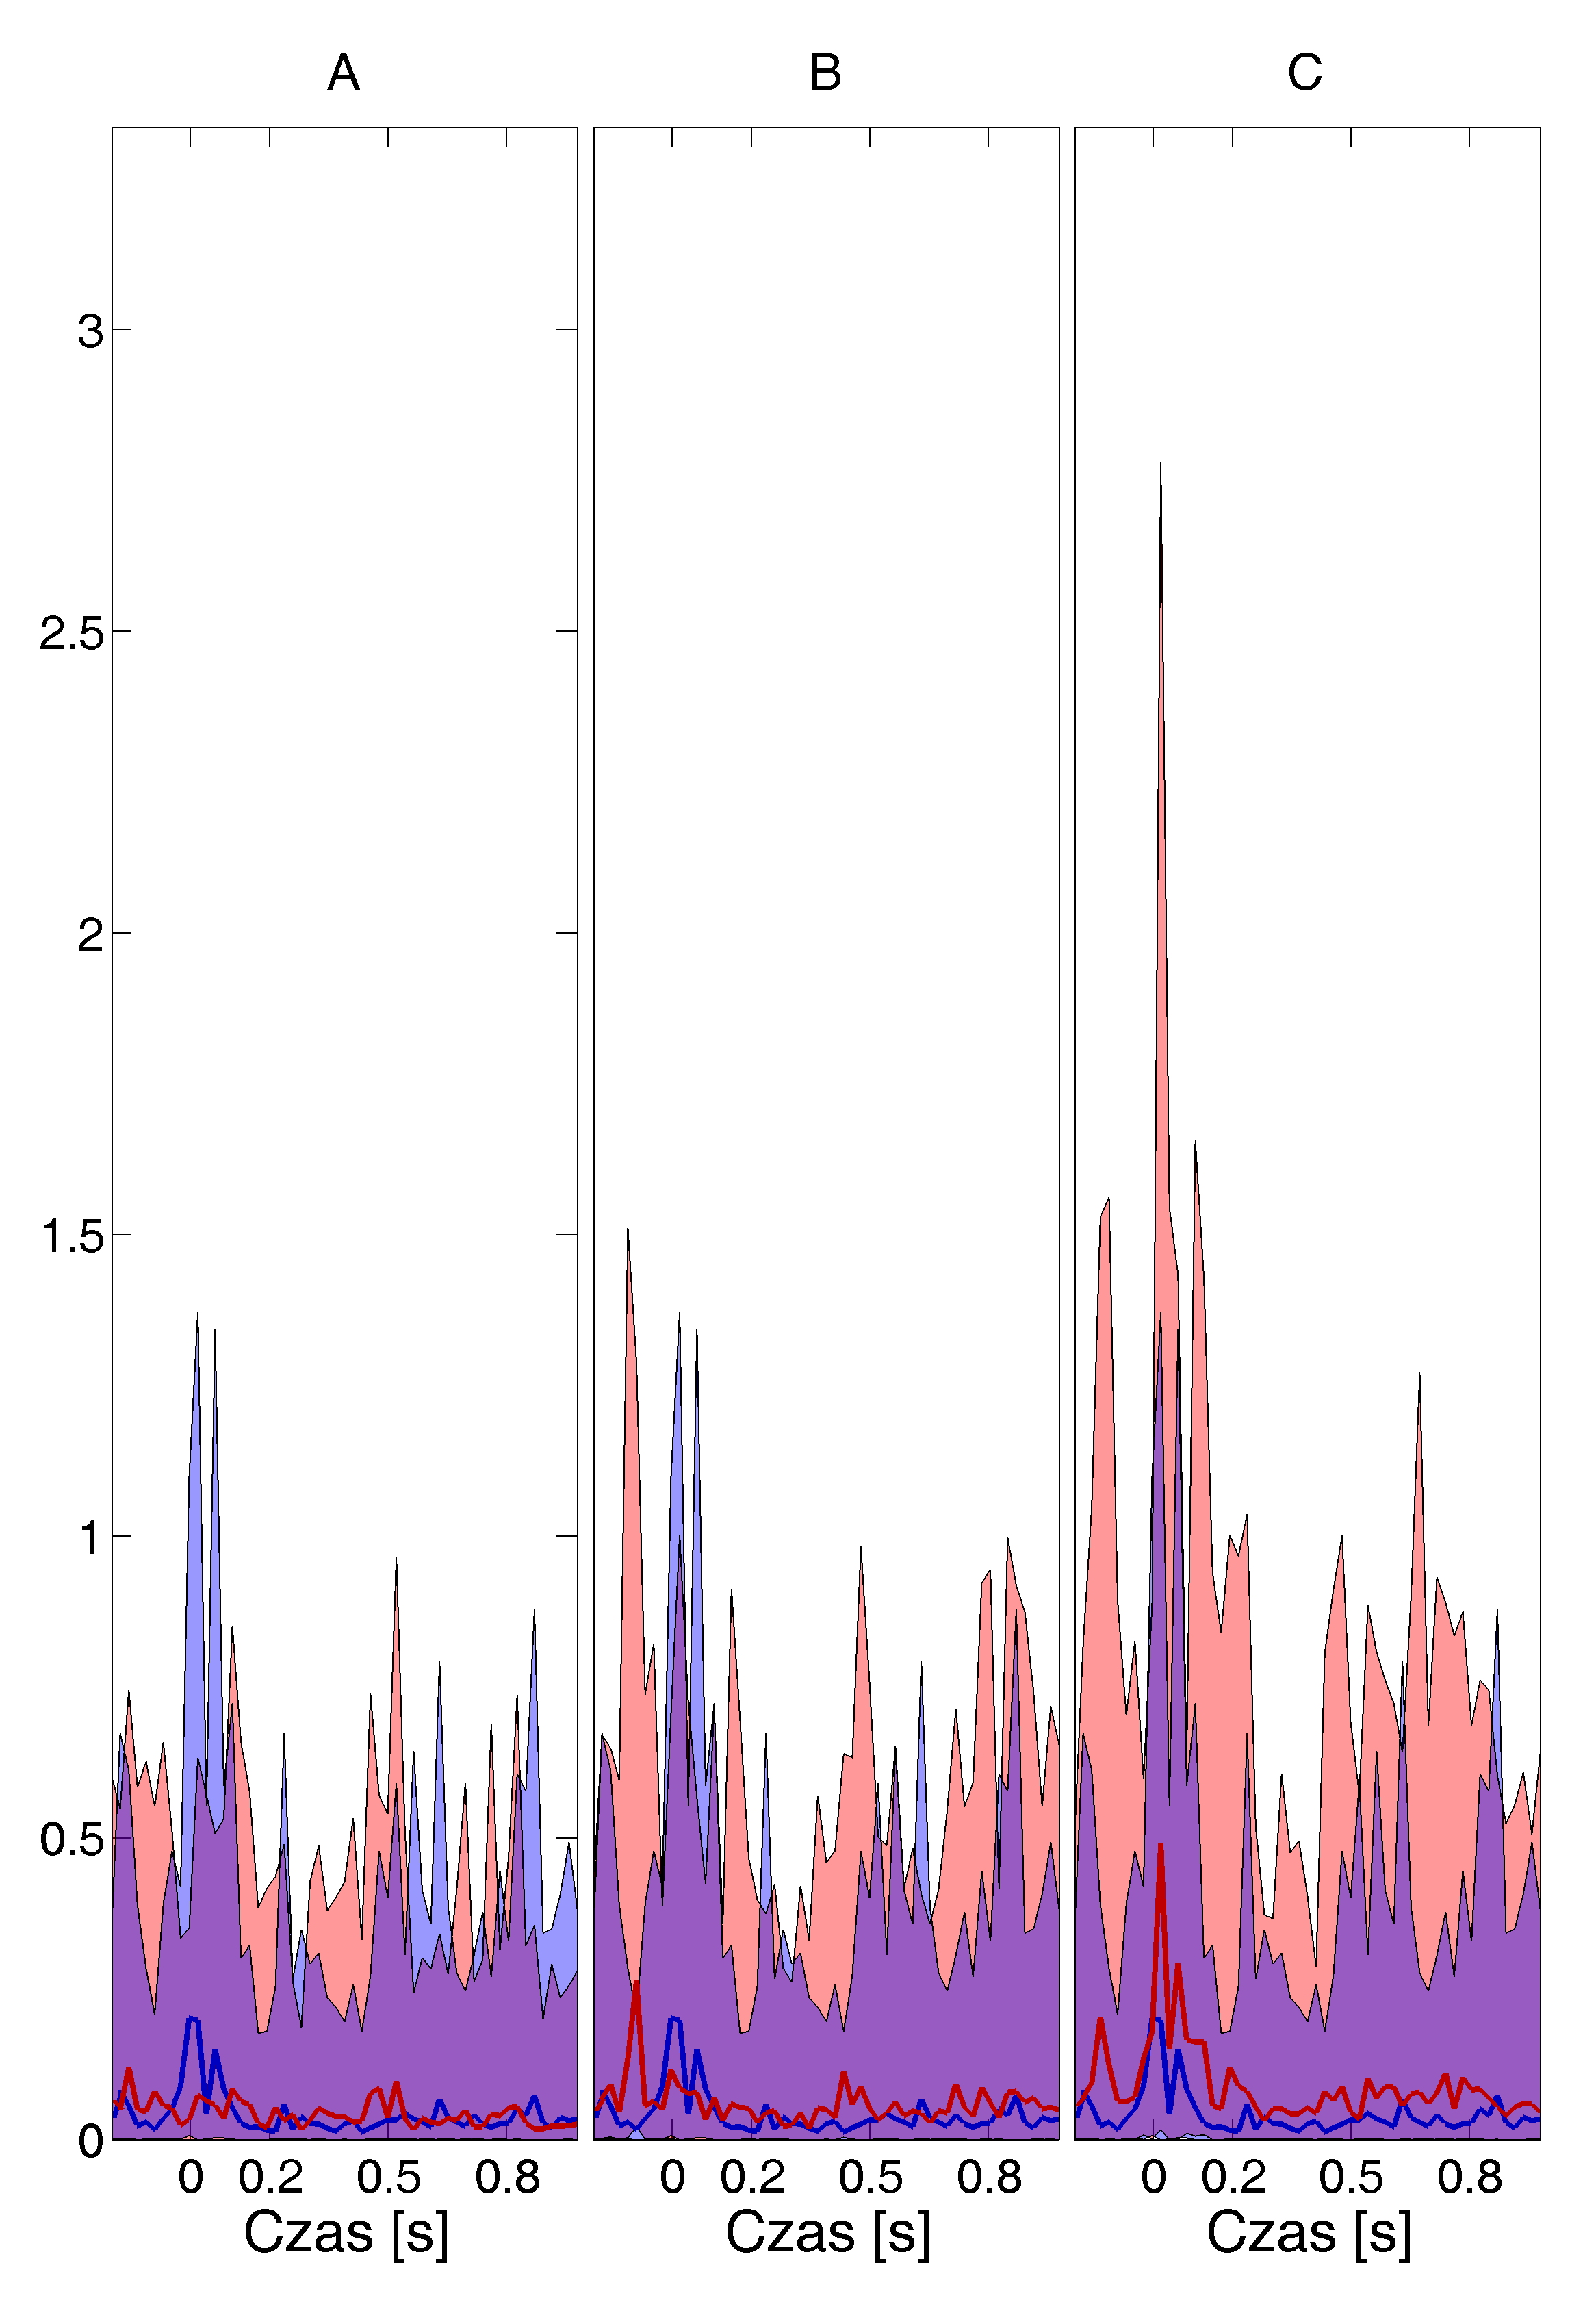
\includegraphics[width=1.\linewidth]{kontrola15_20-40_z_CxC8_do_LGN82.png}
			\caption{Bez stymulacji elektrycznej}
			\label{rys:20_40_kon_CxC_LGN}
		\end{subfigure}%
		\begin{subfigure}{.5\textwidth}
			\centering
			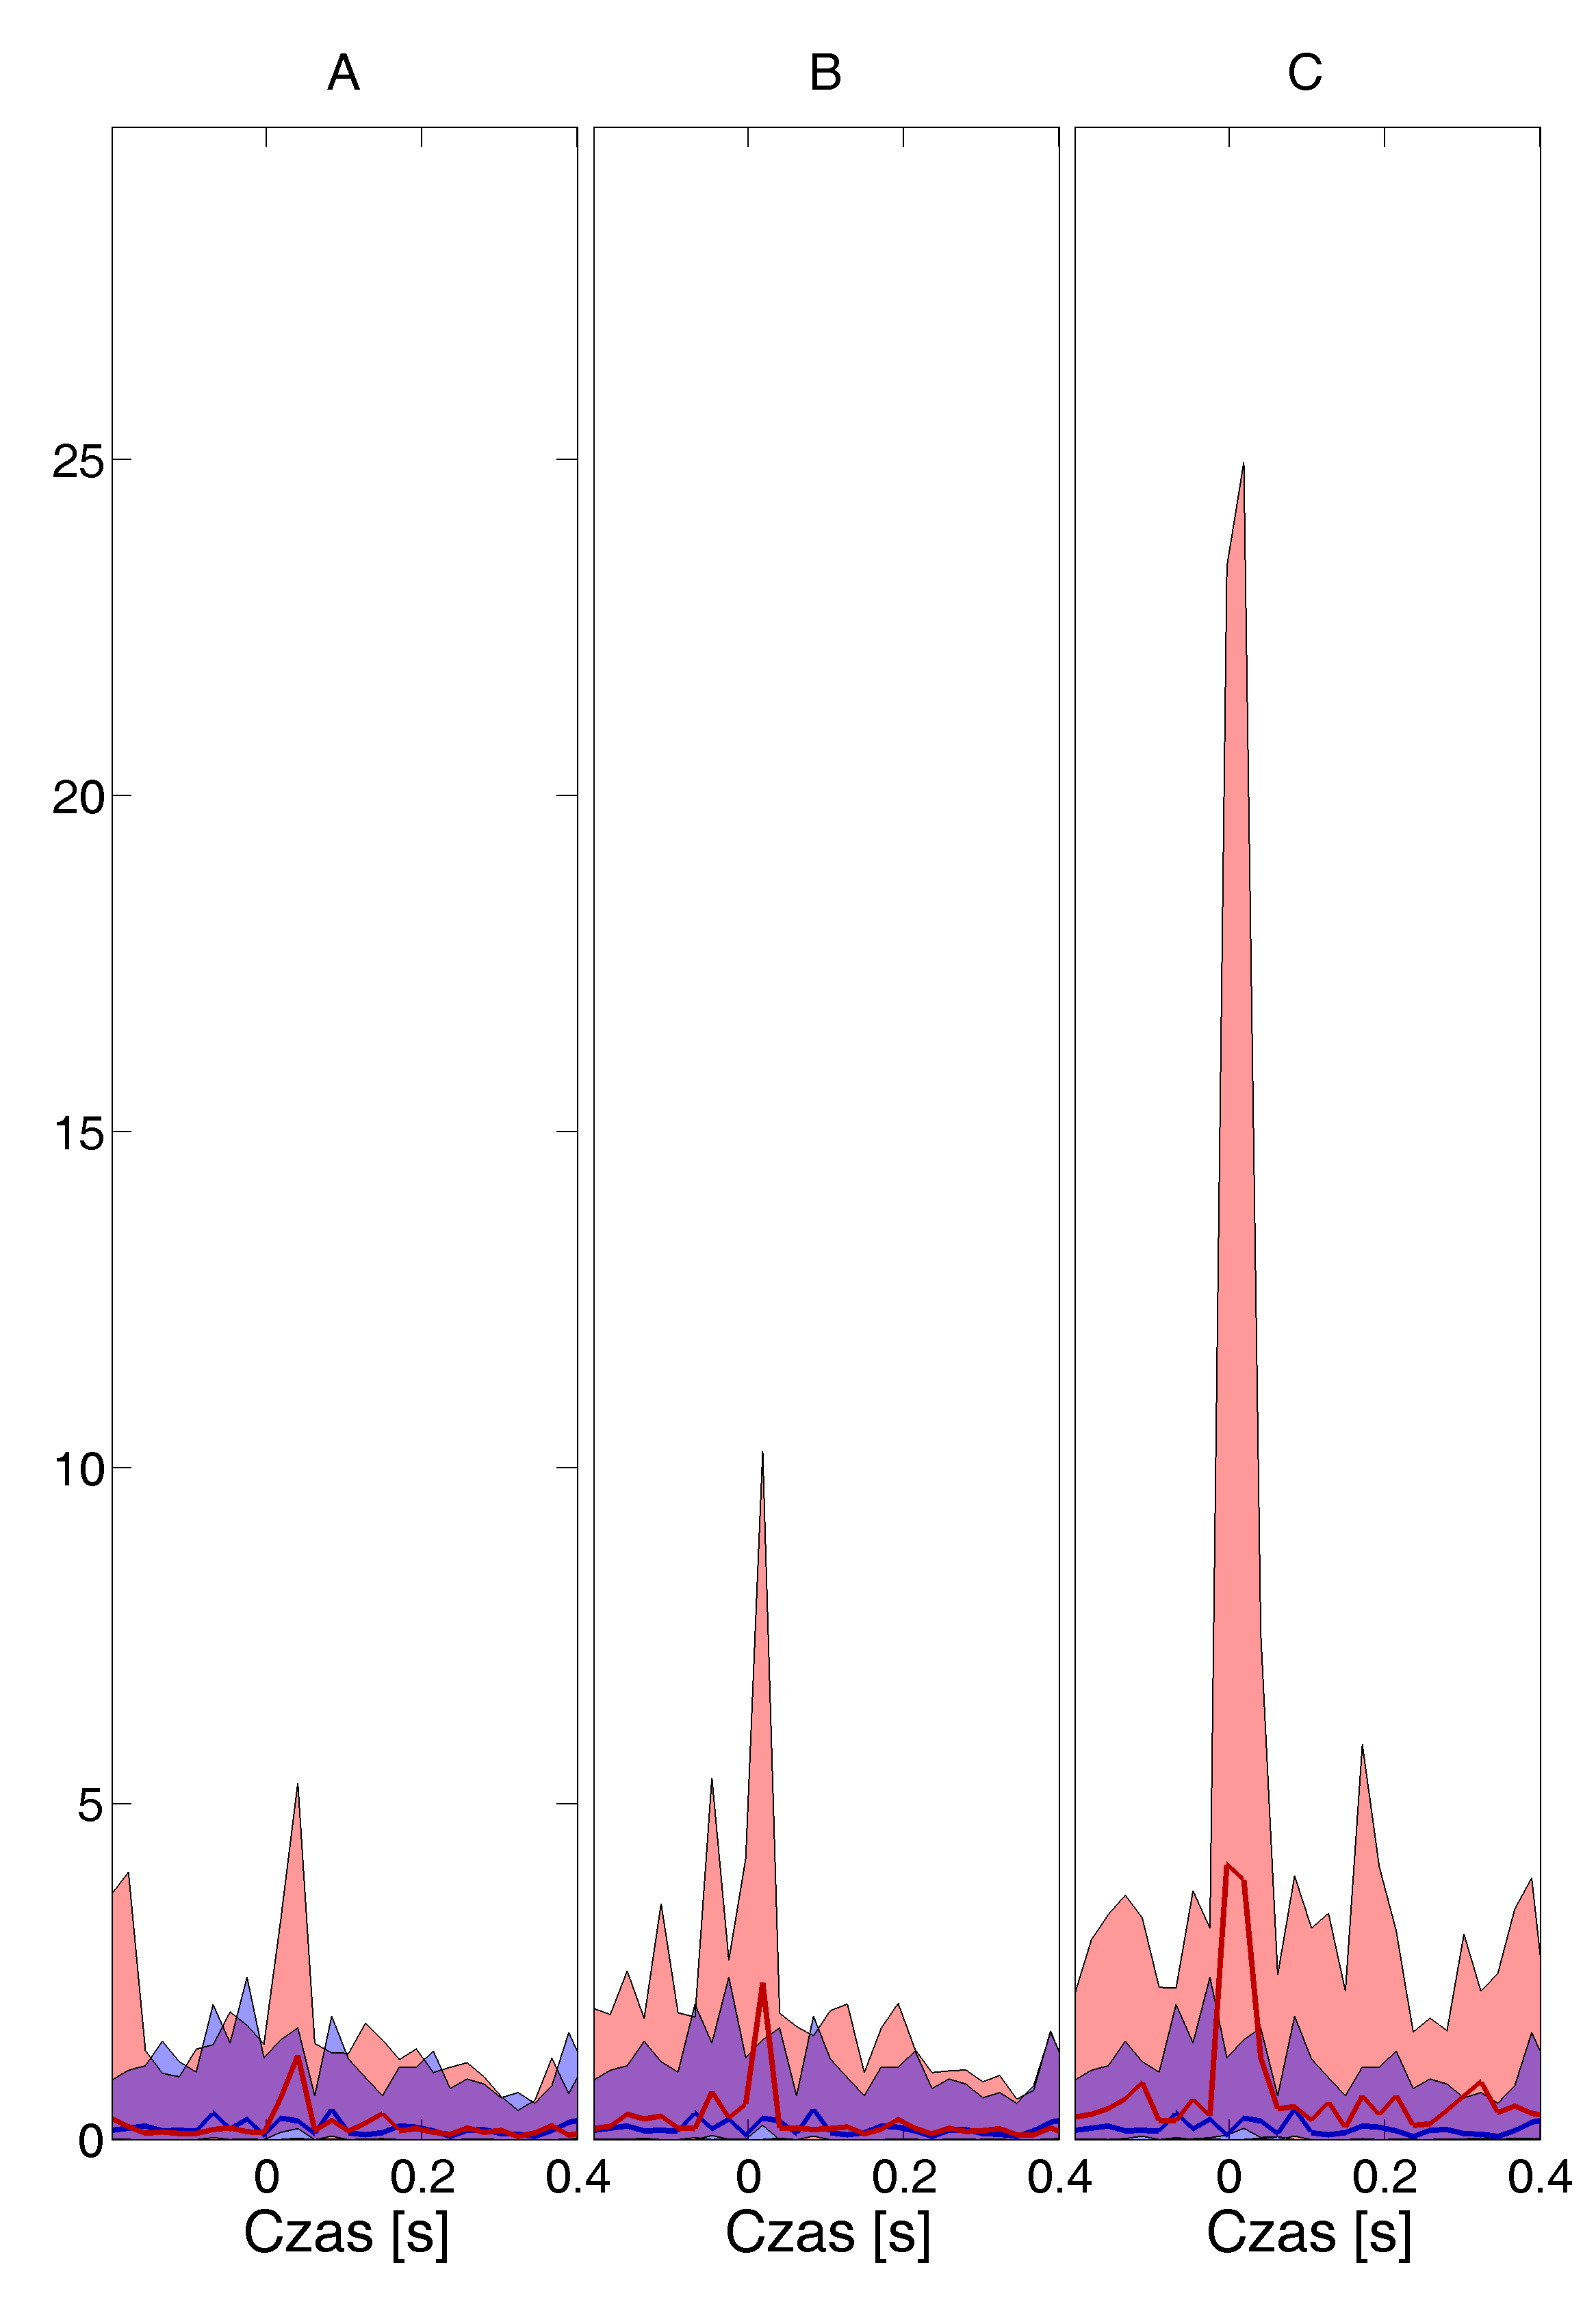
\includegraphics[width=1.\linewidth]{beta3_20-40_z_CxC5_do_LGN42.png}
			\caption{Po stymulacji elektrycznej}
			\label{rys:20_40_beta_CxC_LGN}
		\end{subfigure}
		\caption{Przedstawienie danych z różnych eksperymentów w paśmie 20-40 Hz.}
		\label{rys:20_40_CxC_LGN}
	\end{figure}
	\FloatBarrier
	%\newpage
	\subsection{Połączenia z CxC do SC}
	Do analizy wykorzystano kanały: z zestawu A: CxC8 i SC4 oraz z zestawu B: CxC5 i SC4.
	Na Rysunku \ref{rys:1_10_CxC_SC} przedstawiono wartości funkcji NDTF dla zakresu częstości 1-10 Hz. Dla danych z zestawu A (Rysunek \ref{rys:1_10_kon_CxC_SC}) nie widać wzmocnienia połączeń po kolejnych godzinach treningu względem kontroli. Natomiast dla danych z eksperymentu B (Rysunek \ref{rys:1_10_beta_CxC_SC}) dla pierwszej i drugiej godziny treningu, widoczne są piki w 0 s, co najprawdopodobniej jest wynikiem artefaktów związanych z bodźcem. Dla trzeciej godziny treningu widoczny jest wzrost wartości funkcji NDTF względem danych kontrolnych w czasie 0,2 s.
	\begin{figure}[h]
		\begin{subfigure}{.5\textwidth}
			\centering
			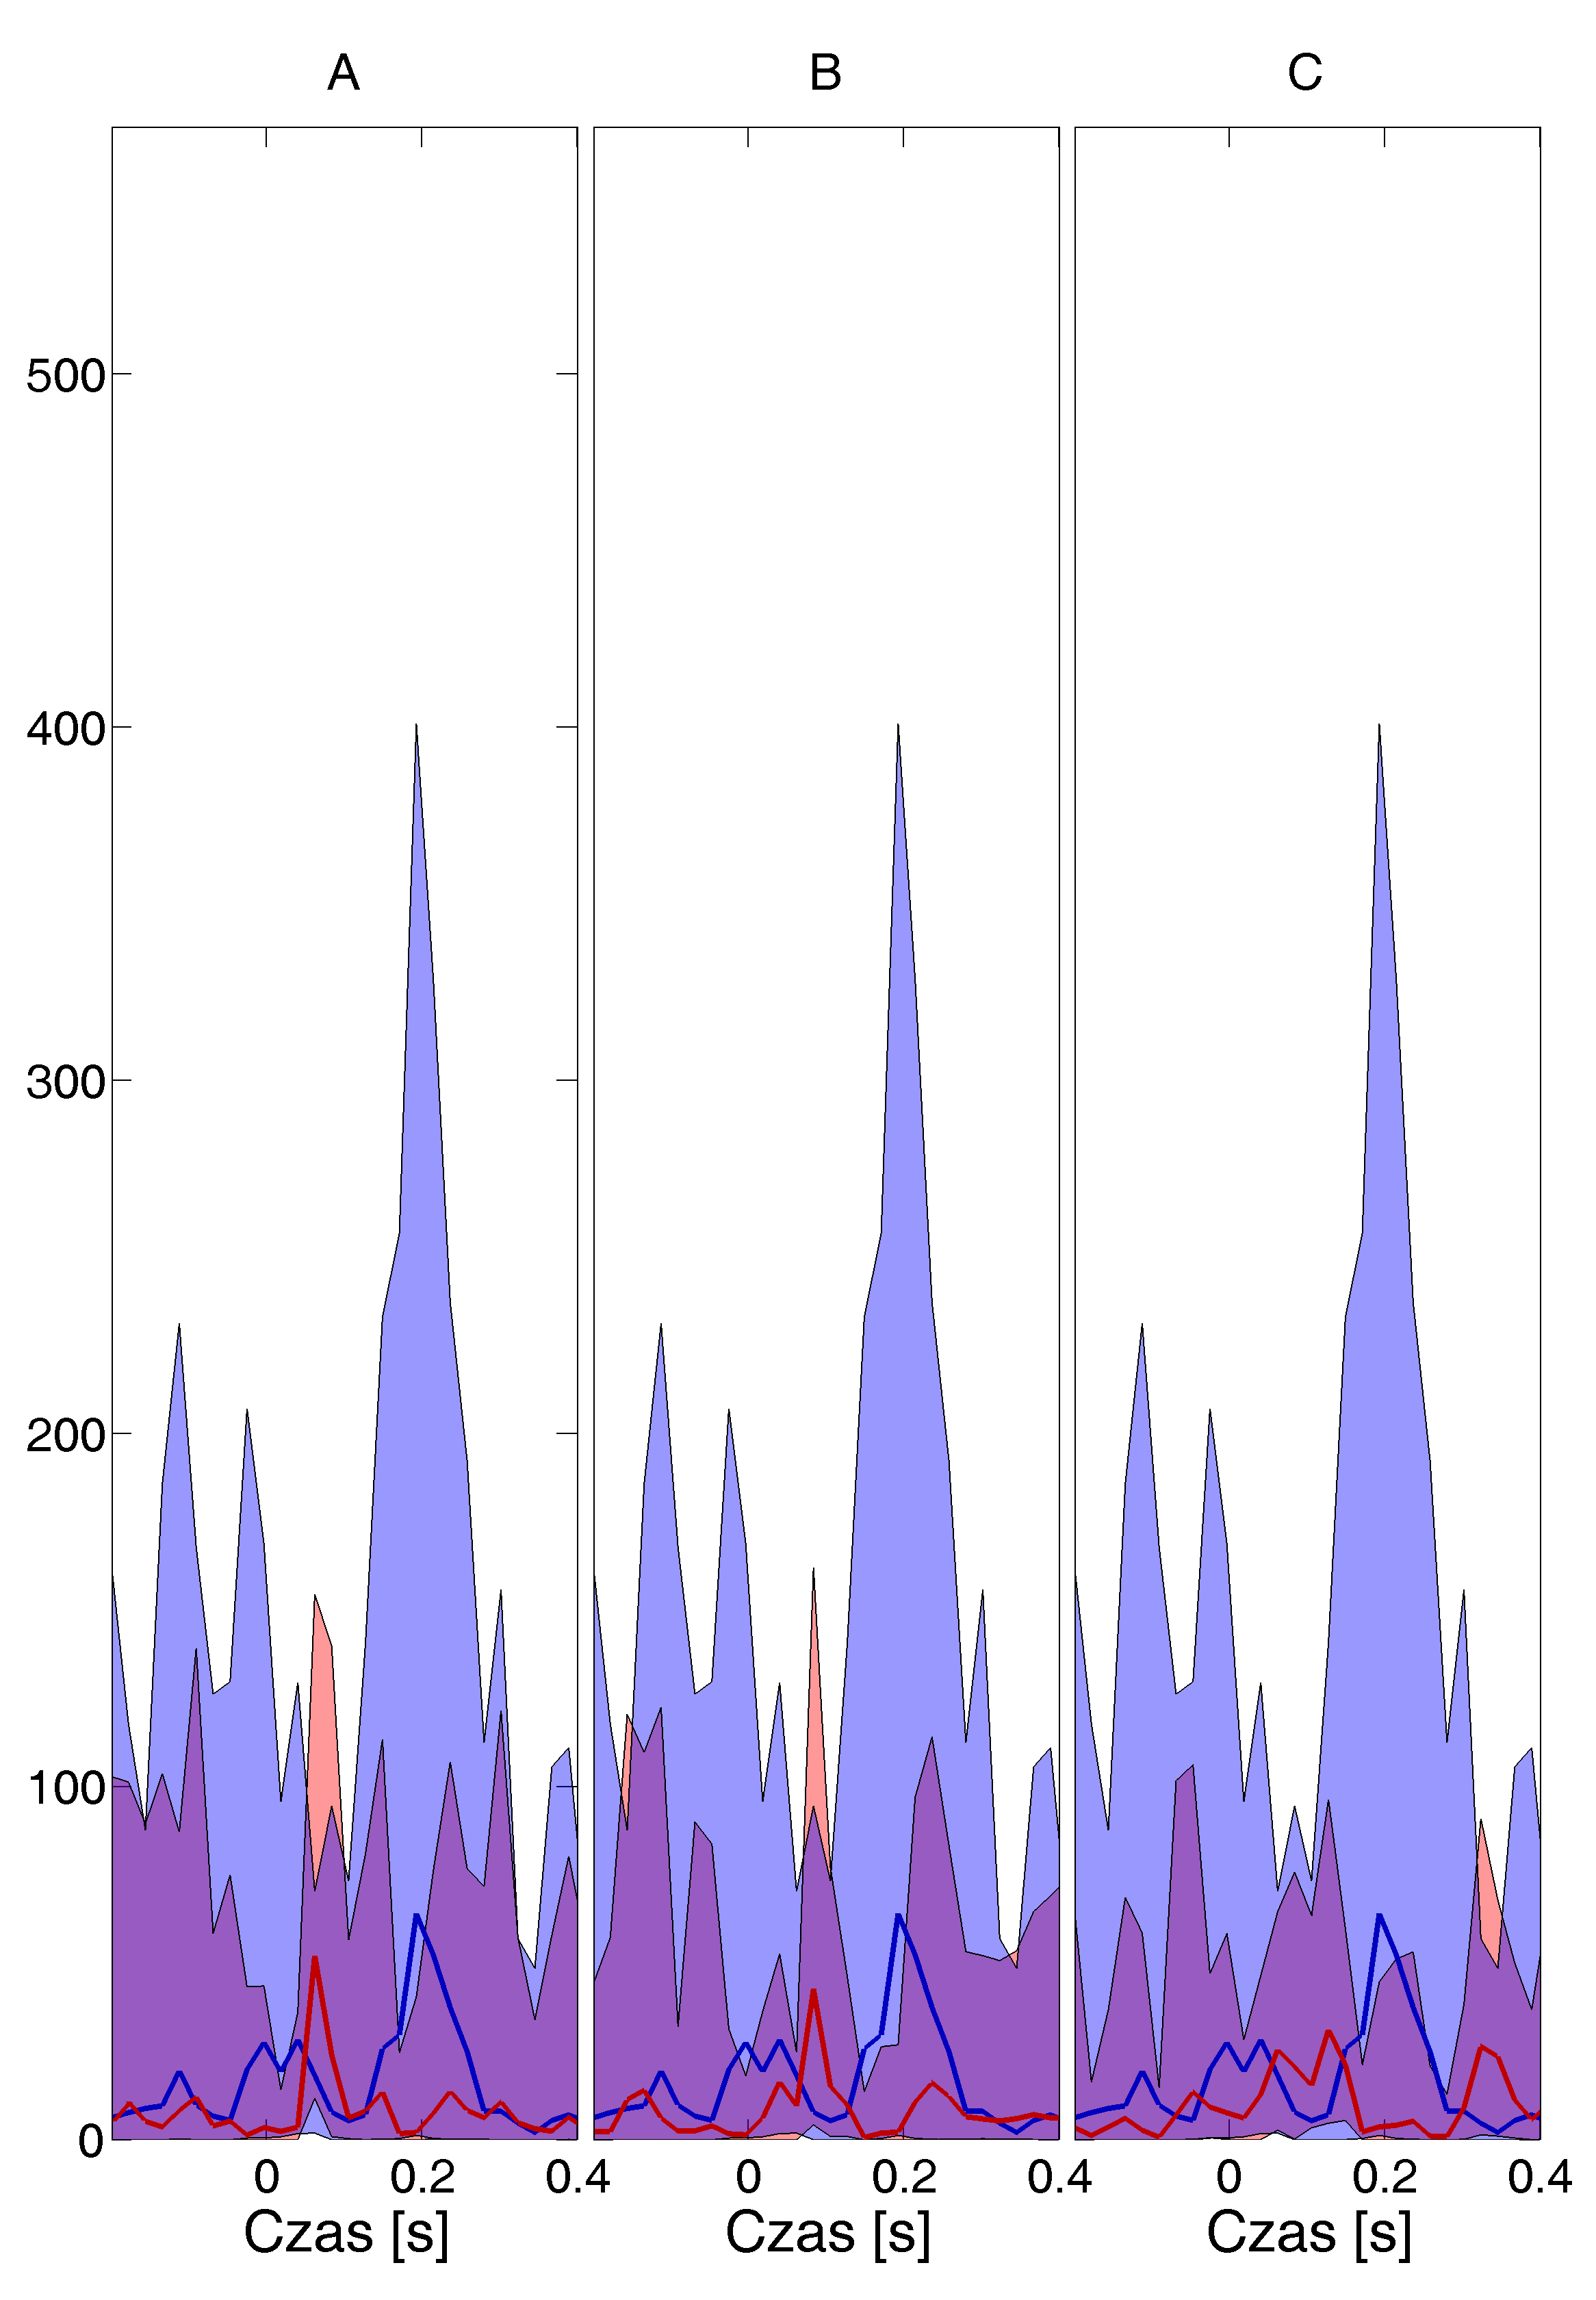
\includegraphics[width=1.\linewidth]{kontrola15_1-10_z_CxC8_do_SC42.png}
			\caption{Bez stymulacji elektrycznej}
			\label{rys:1_10_kon_CxC_SC}
		\end{subfigure}%
		\begin{subfigure}{.5\textwidth}
			\centering
			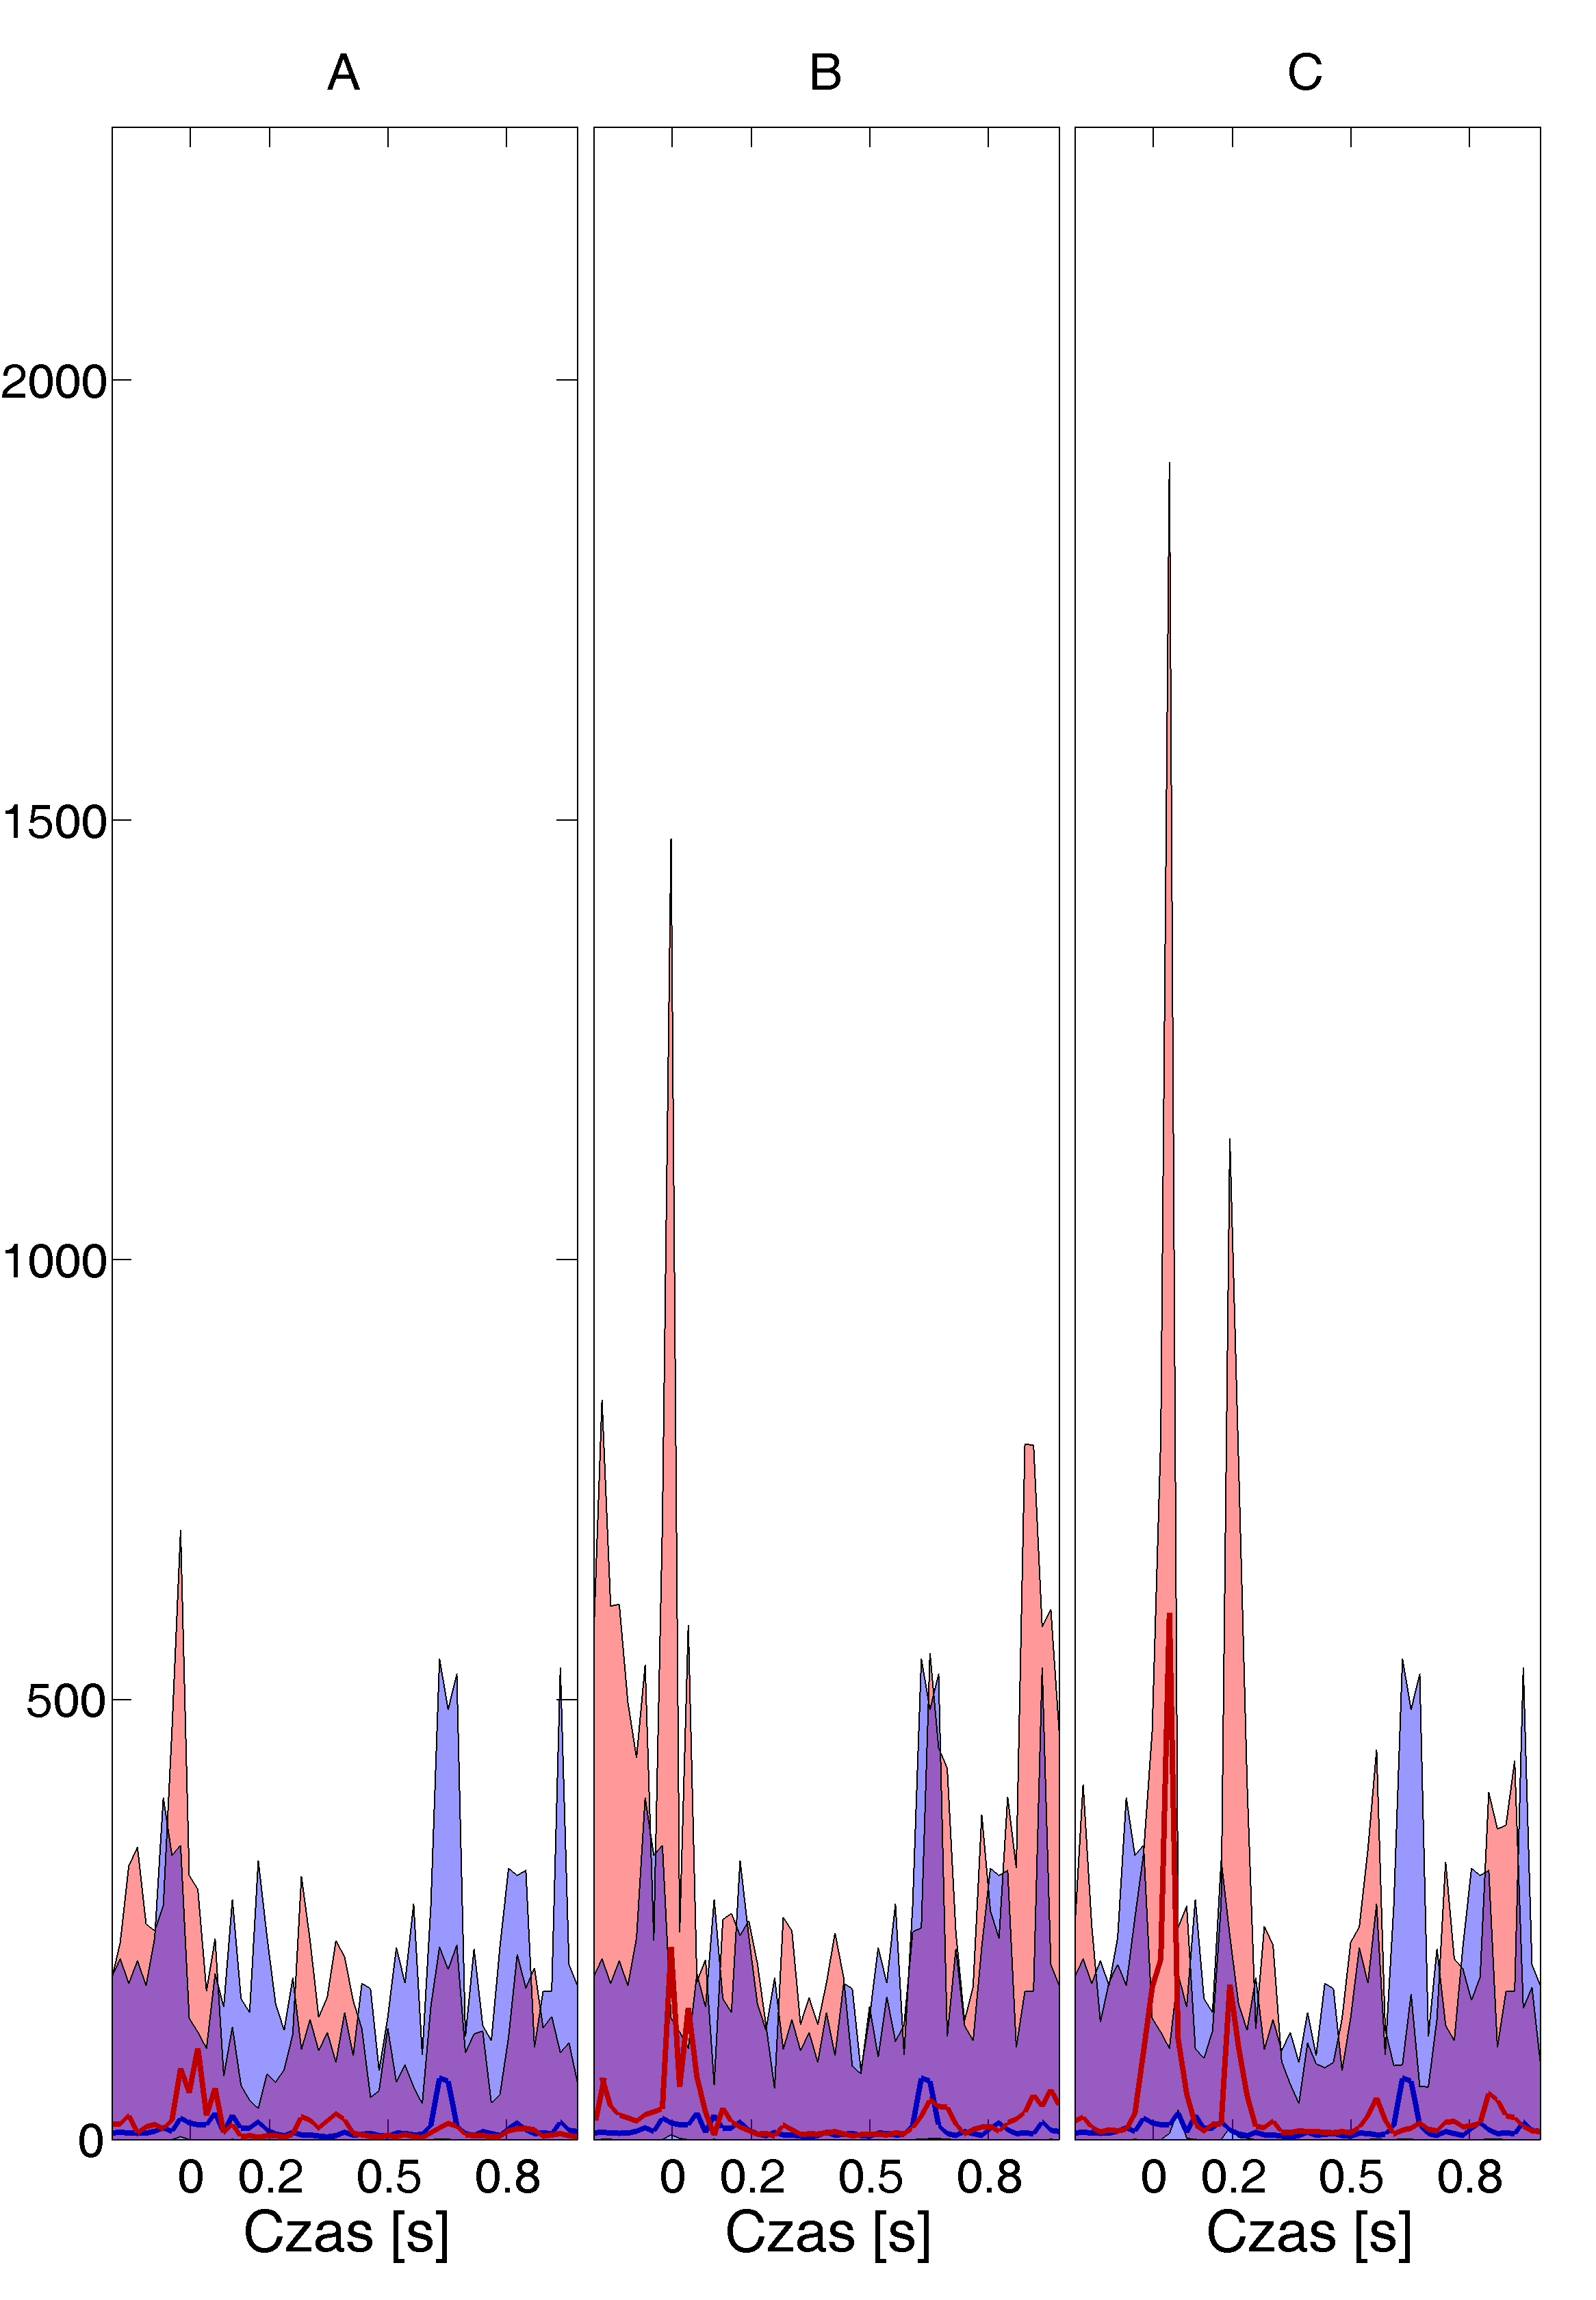
\includegraphics[width=1.\linewidth]{beta3_1-10_z_CxC5_do_SC42.png}
			\caption{Po stymulacji elektrycznej}
			\label{rys:1_10_beta_CxC_SC}
		\end{subfigure}
		\caption{Przedstawienie danych z różnych eksperymentów w paśmie 1-10 Hz.}
		\label{rys:1_10_CxC_SC}
	\end{figure}
	\FloatBarrier
	Na Rysunkach \ref{rys:10_30_CxC_SC} i \ref{rys:20_40_CxC_SC} przedstawiono wartości funkcji NDTF dla odpowiednio 10-30 Hz oraz 20-40 Hz. Dla obu zestawów danych widoczny jest pik w 0-0,1 s. Jednakże w eksperymentu A (Rysunki \ref{rys:10_30_kon_CxC_SC} i \ref{rys:20_40_kon_CxC_SC}) funkcja NDTF przyjmuje wysokie wartości również dla danych kontrolnych. Dla danych z eksperymentu B (Rysunki \ref{rys:10_30_beta_CxC_SC} i \ref{rys:20_40_beta_CxC_SC}) różnica między wartościami funkcji NDTF po każdej godzinie treningu a danymi kontrolnymi w czasie 0-0,1~s jest znacznie większa niż dla danych z eksperymentu A.
	\begin{figure}[h]
		\begin{subfigure}{.5\textwidth}
			\centering
			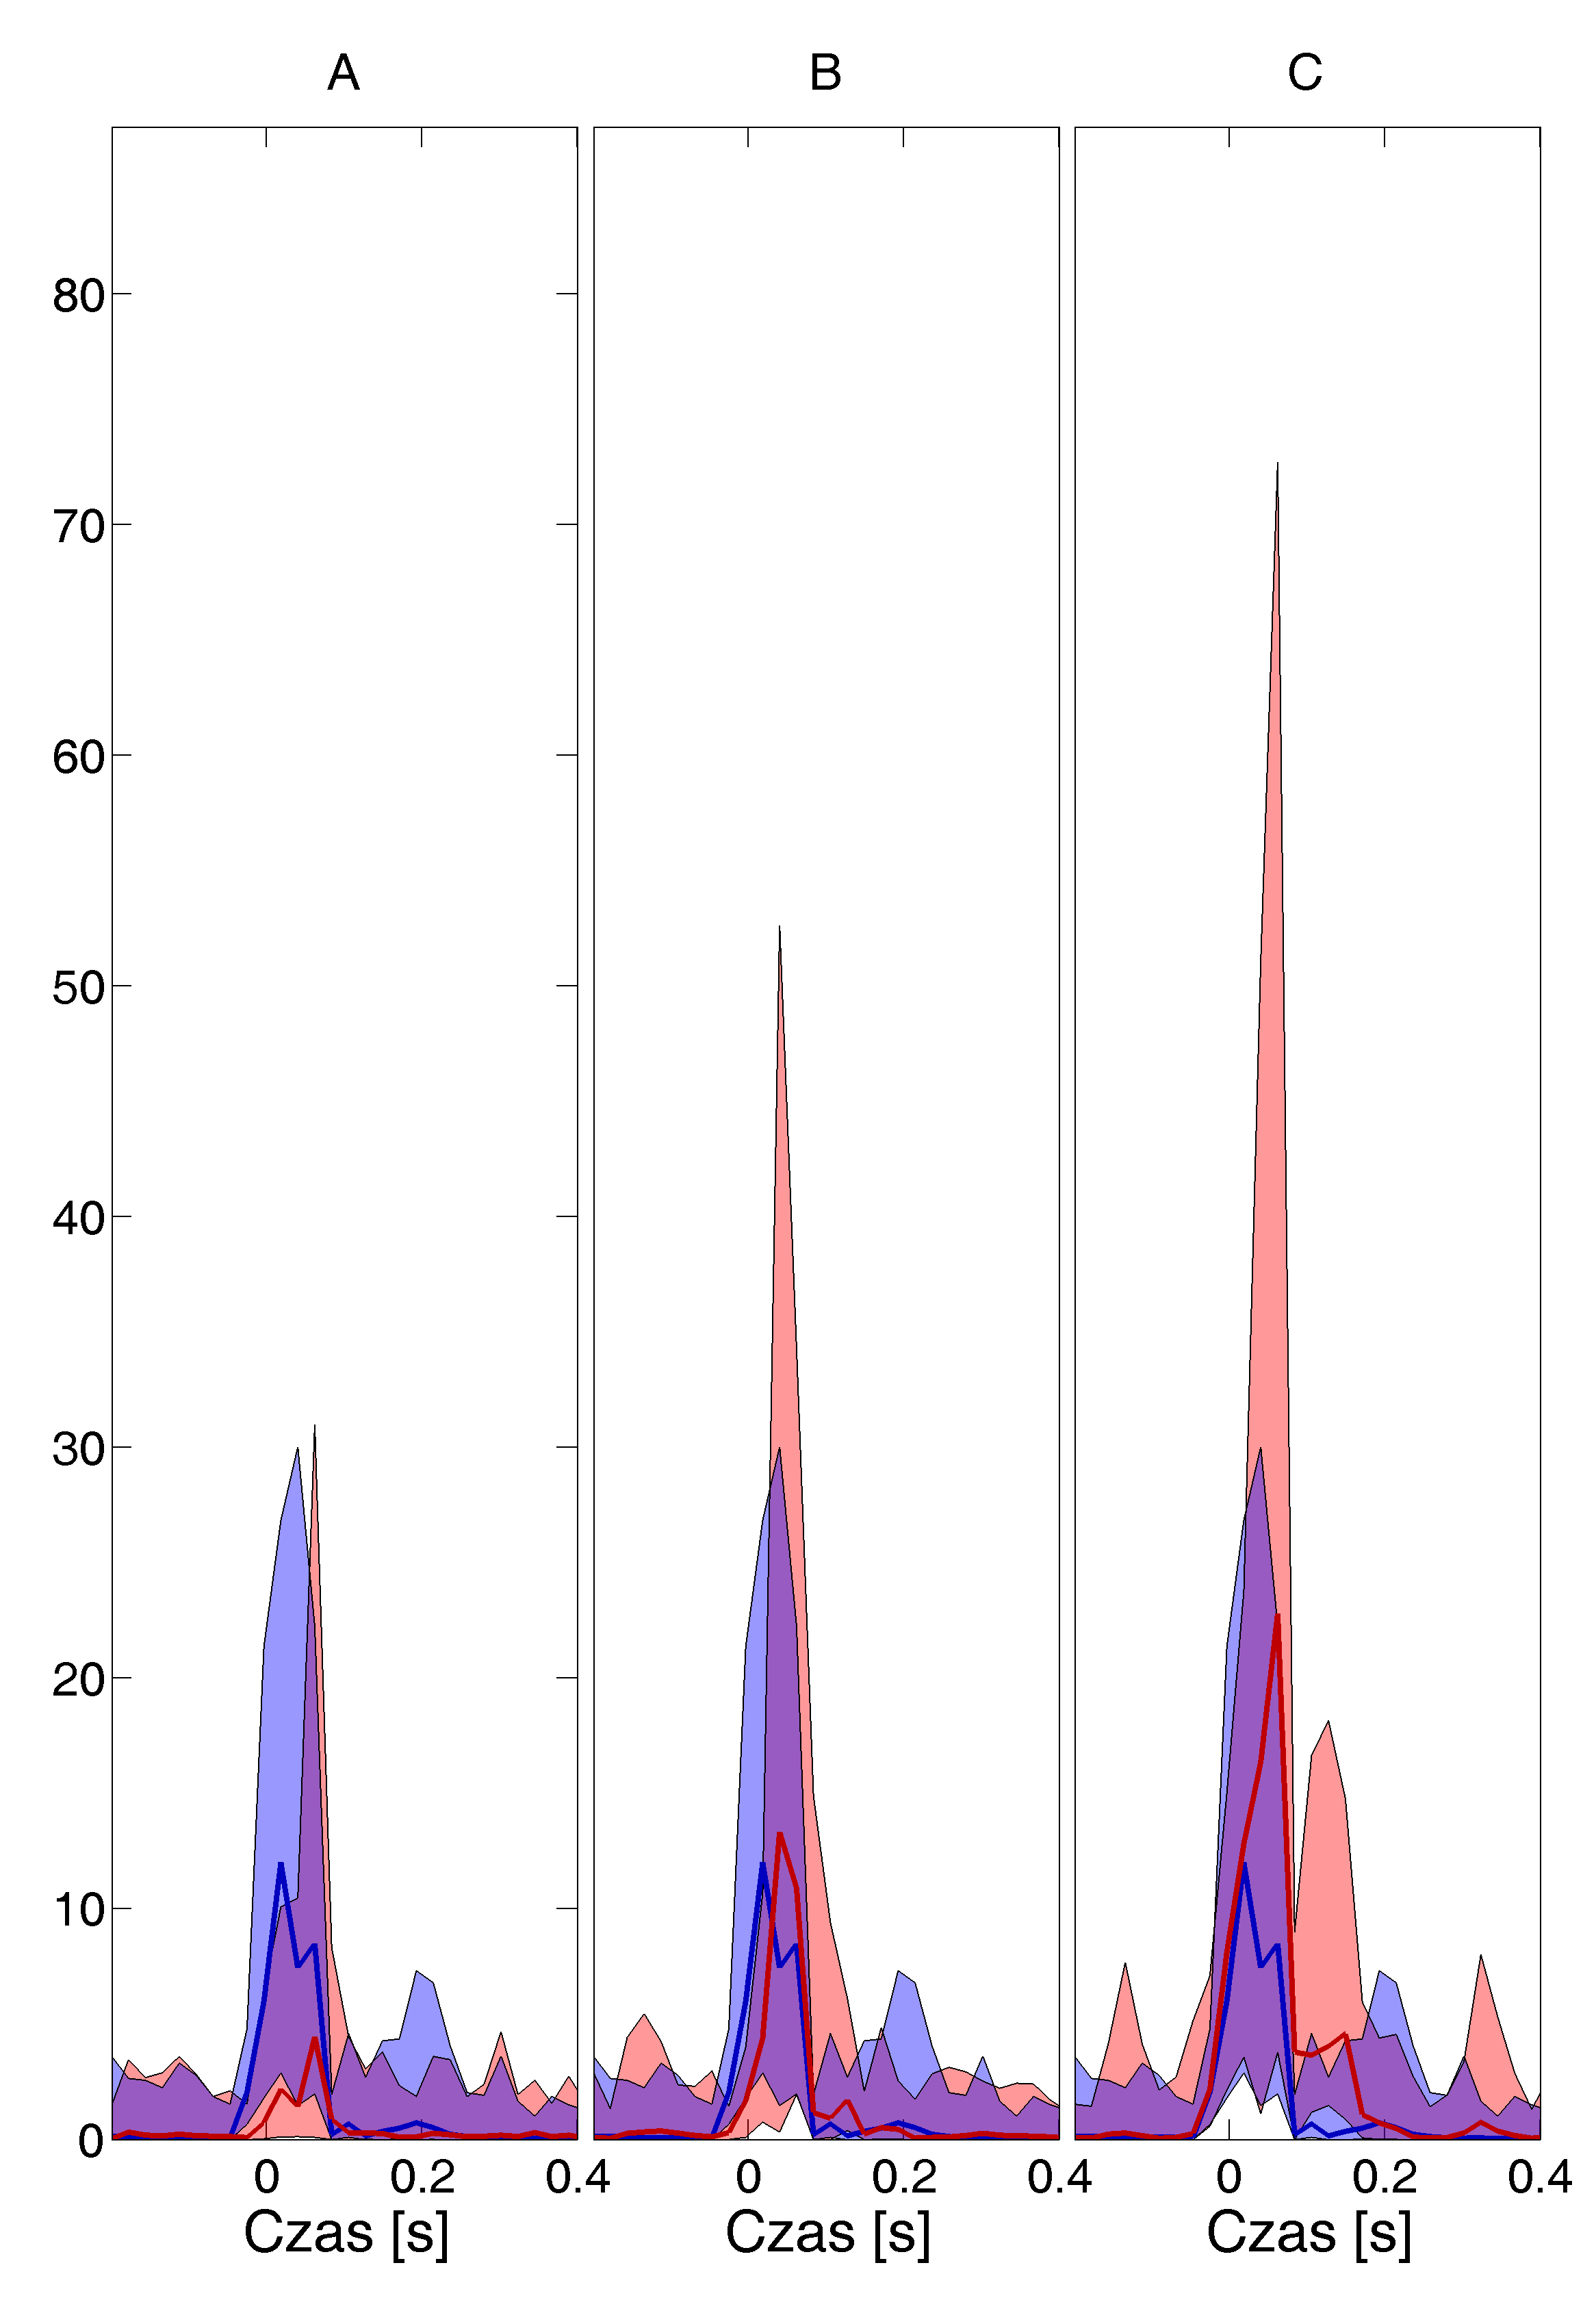
\includegraphics[width=1.\linewidth]{kontrola15_10-30_z_CxC8_do_SC42.png}
			\caption{Bez stymulacji elektrycznej}
			\label{rys:10_30_kon_CxC_SC}
		\end{subfigure}%
		\begin{subfigure}{.5\textwidth}
			\centering
			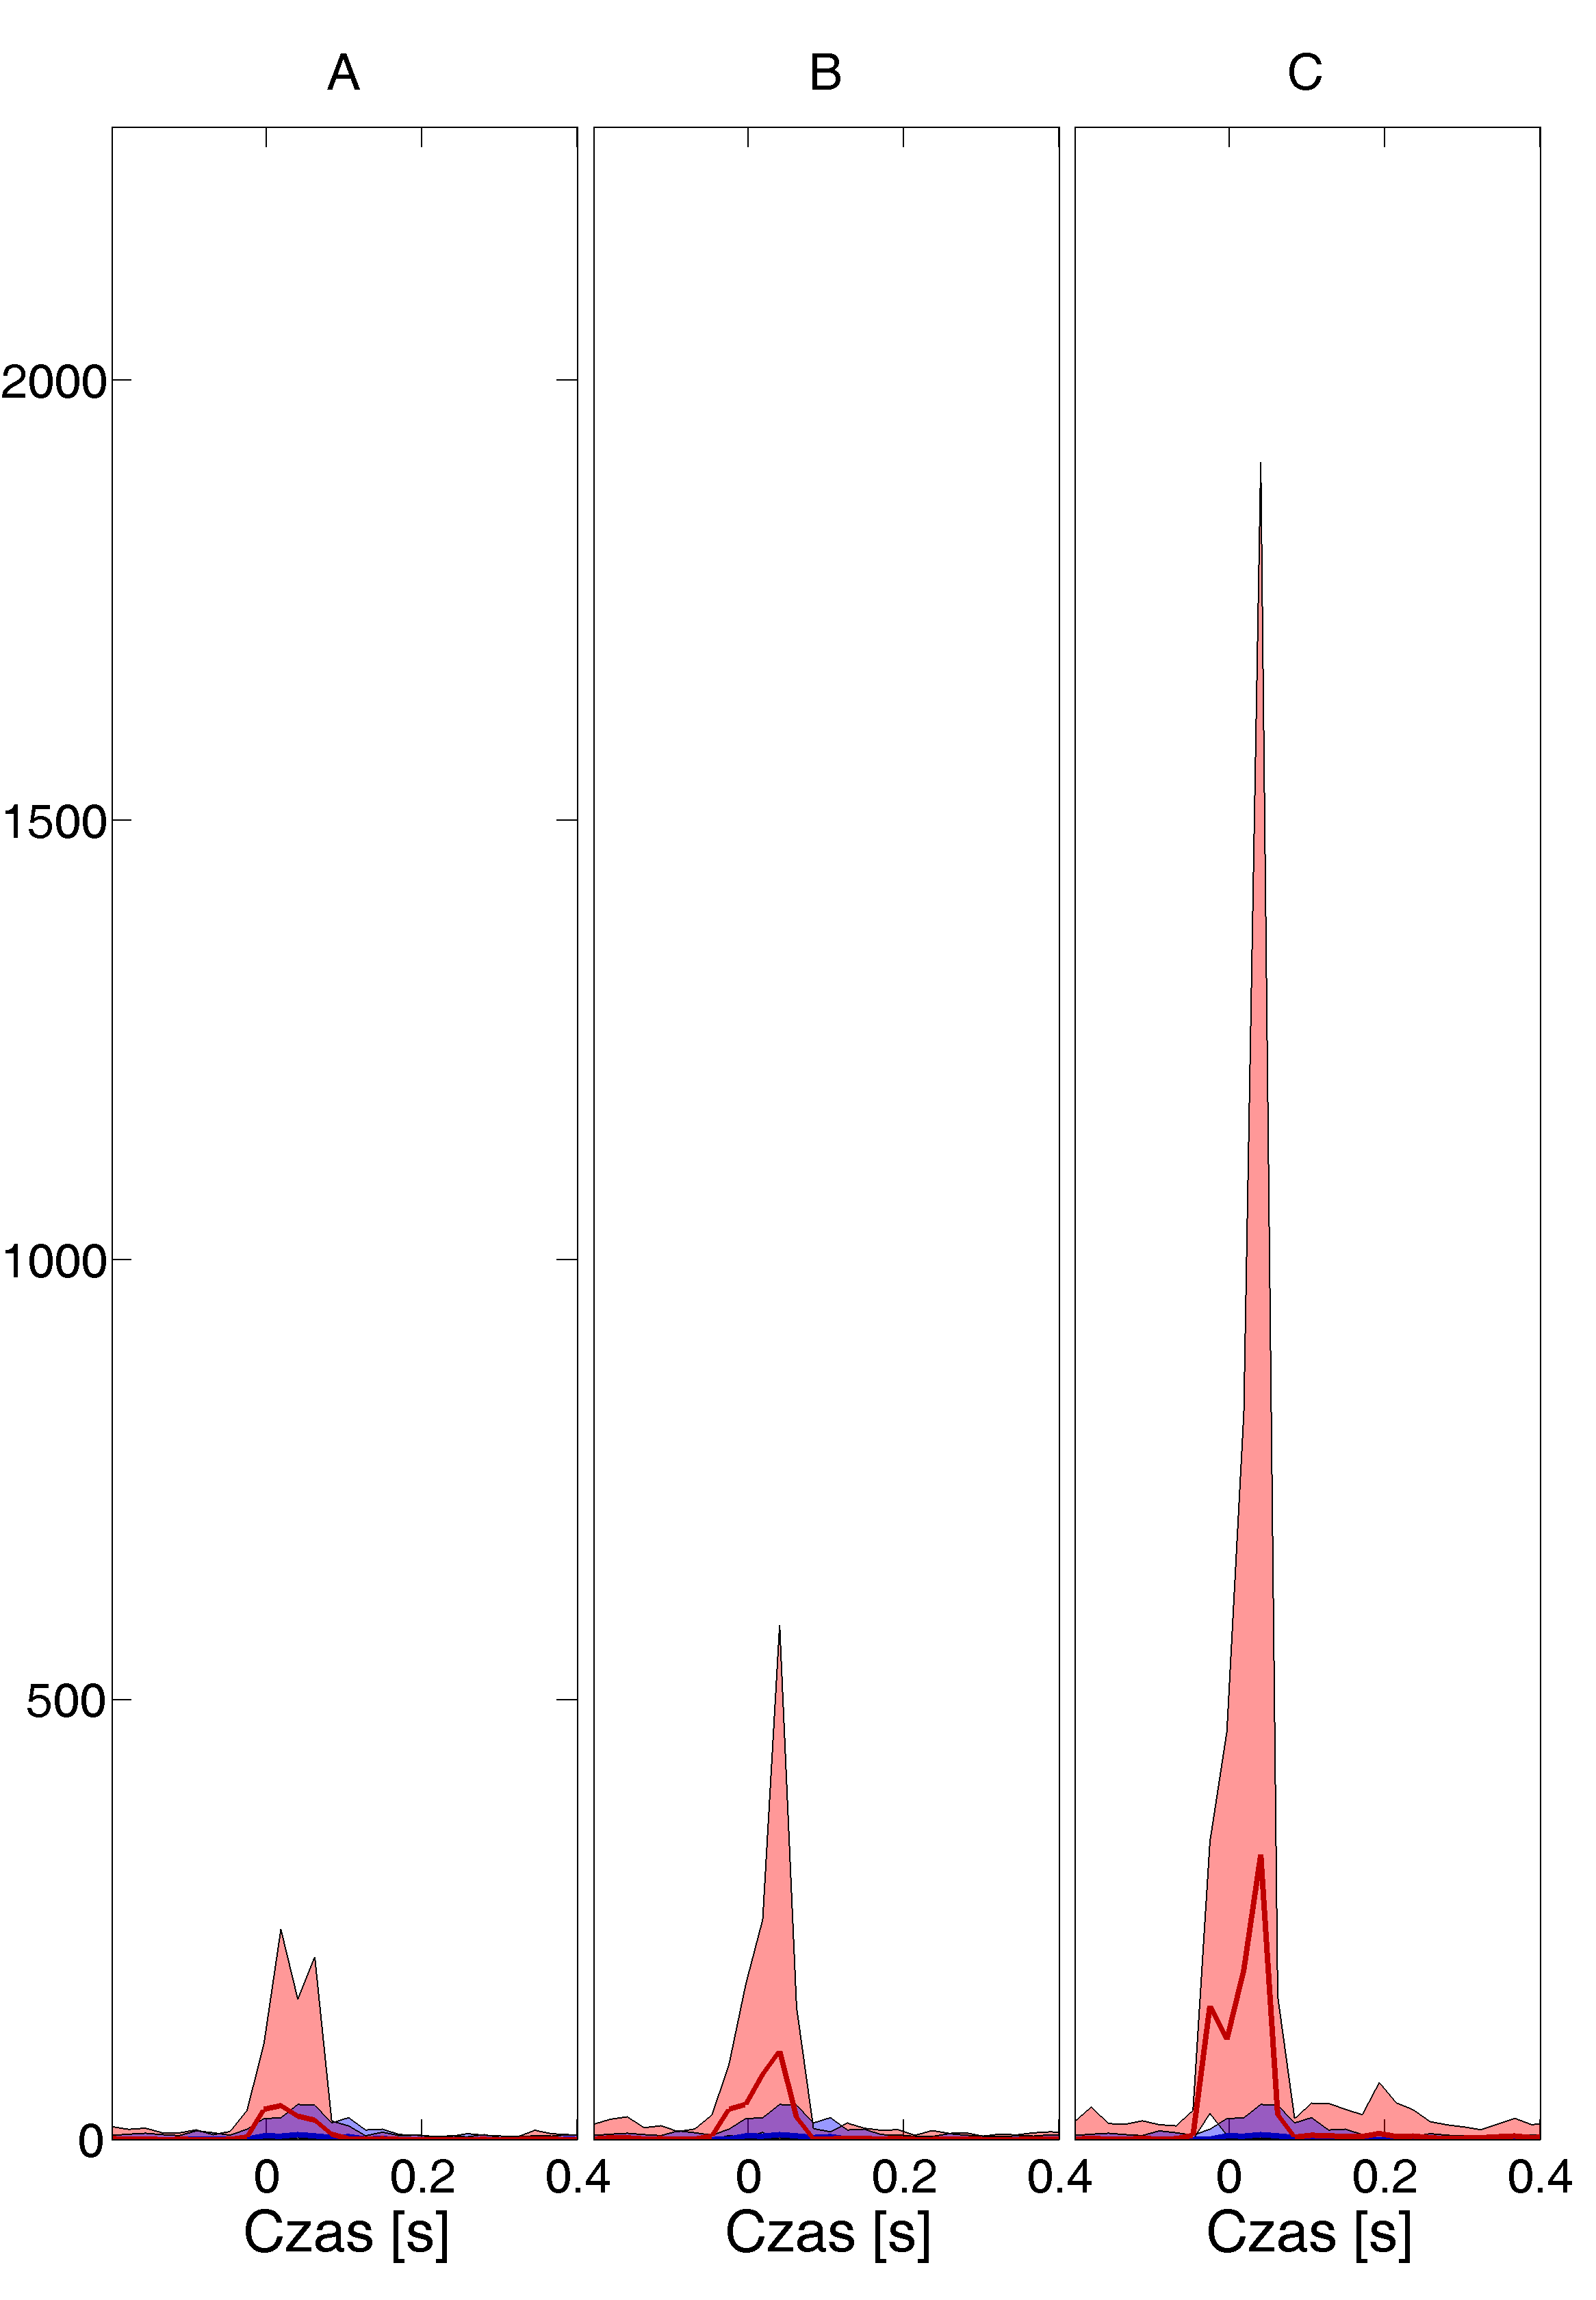
\includegraphics[width=1.\linewidth]{beta3_10-30_z_CxC5_do_SC42.png}
			\caption{Po stymulacji elektrycznej}
			\label{rys:10_30_beta_CxC_SC}
		\end{subfigure}
		\caption{Przedstawienie danych z różnych eksperymentów w paśmie 10-30 Hz.}
		\label{rys:10_30_CxC_SC}
	\end{figure}
	\begin{figure}[h]
		\begin{subfigure}{.5\textwidth}
			\centering
			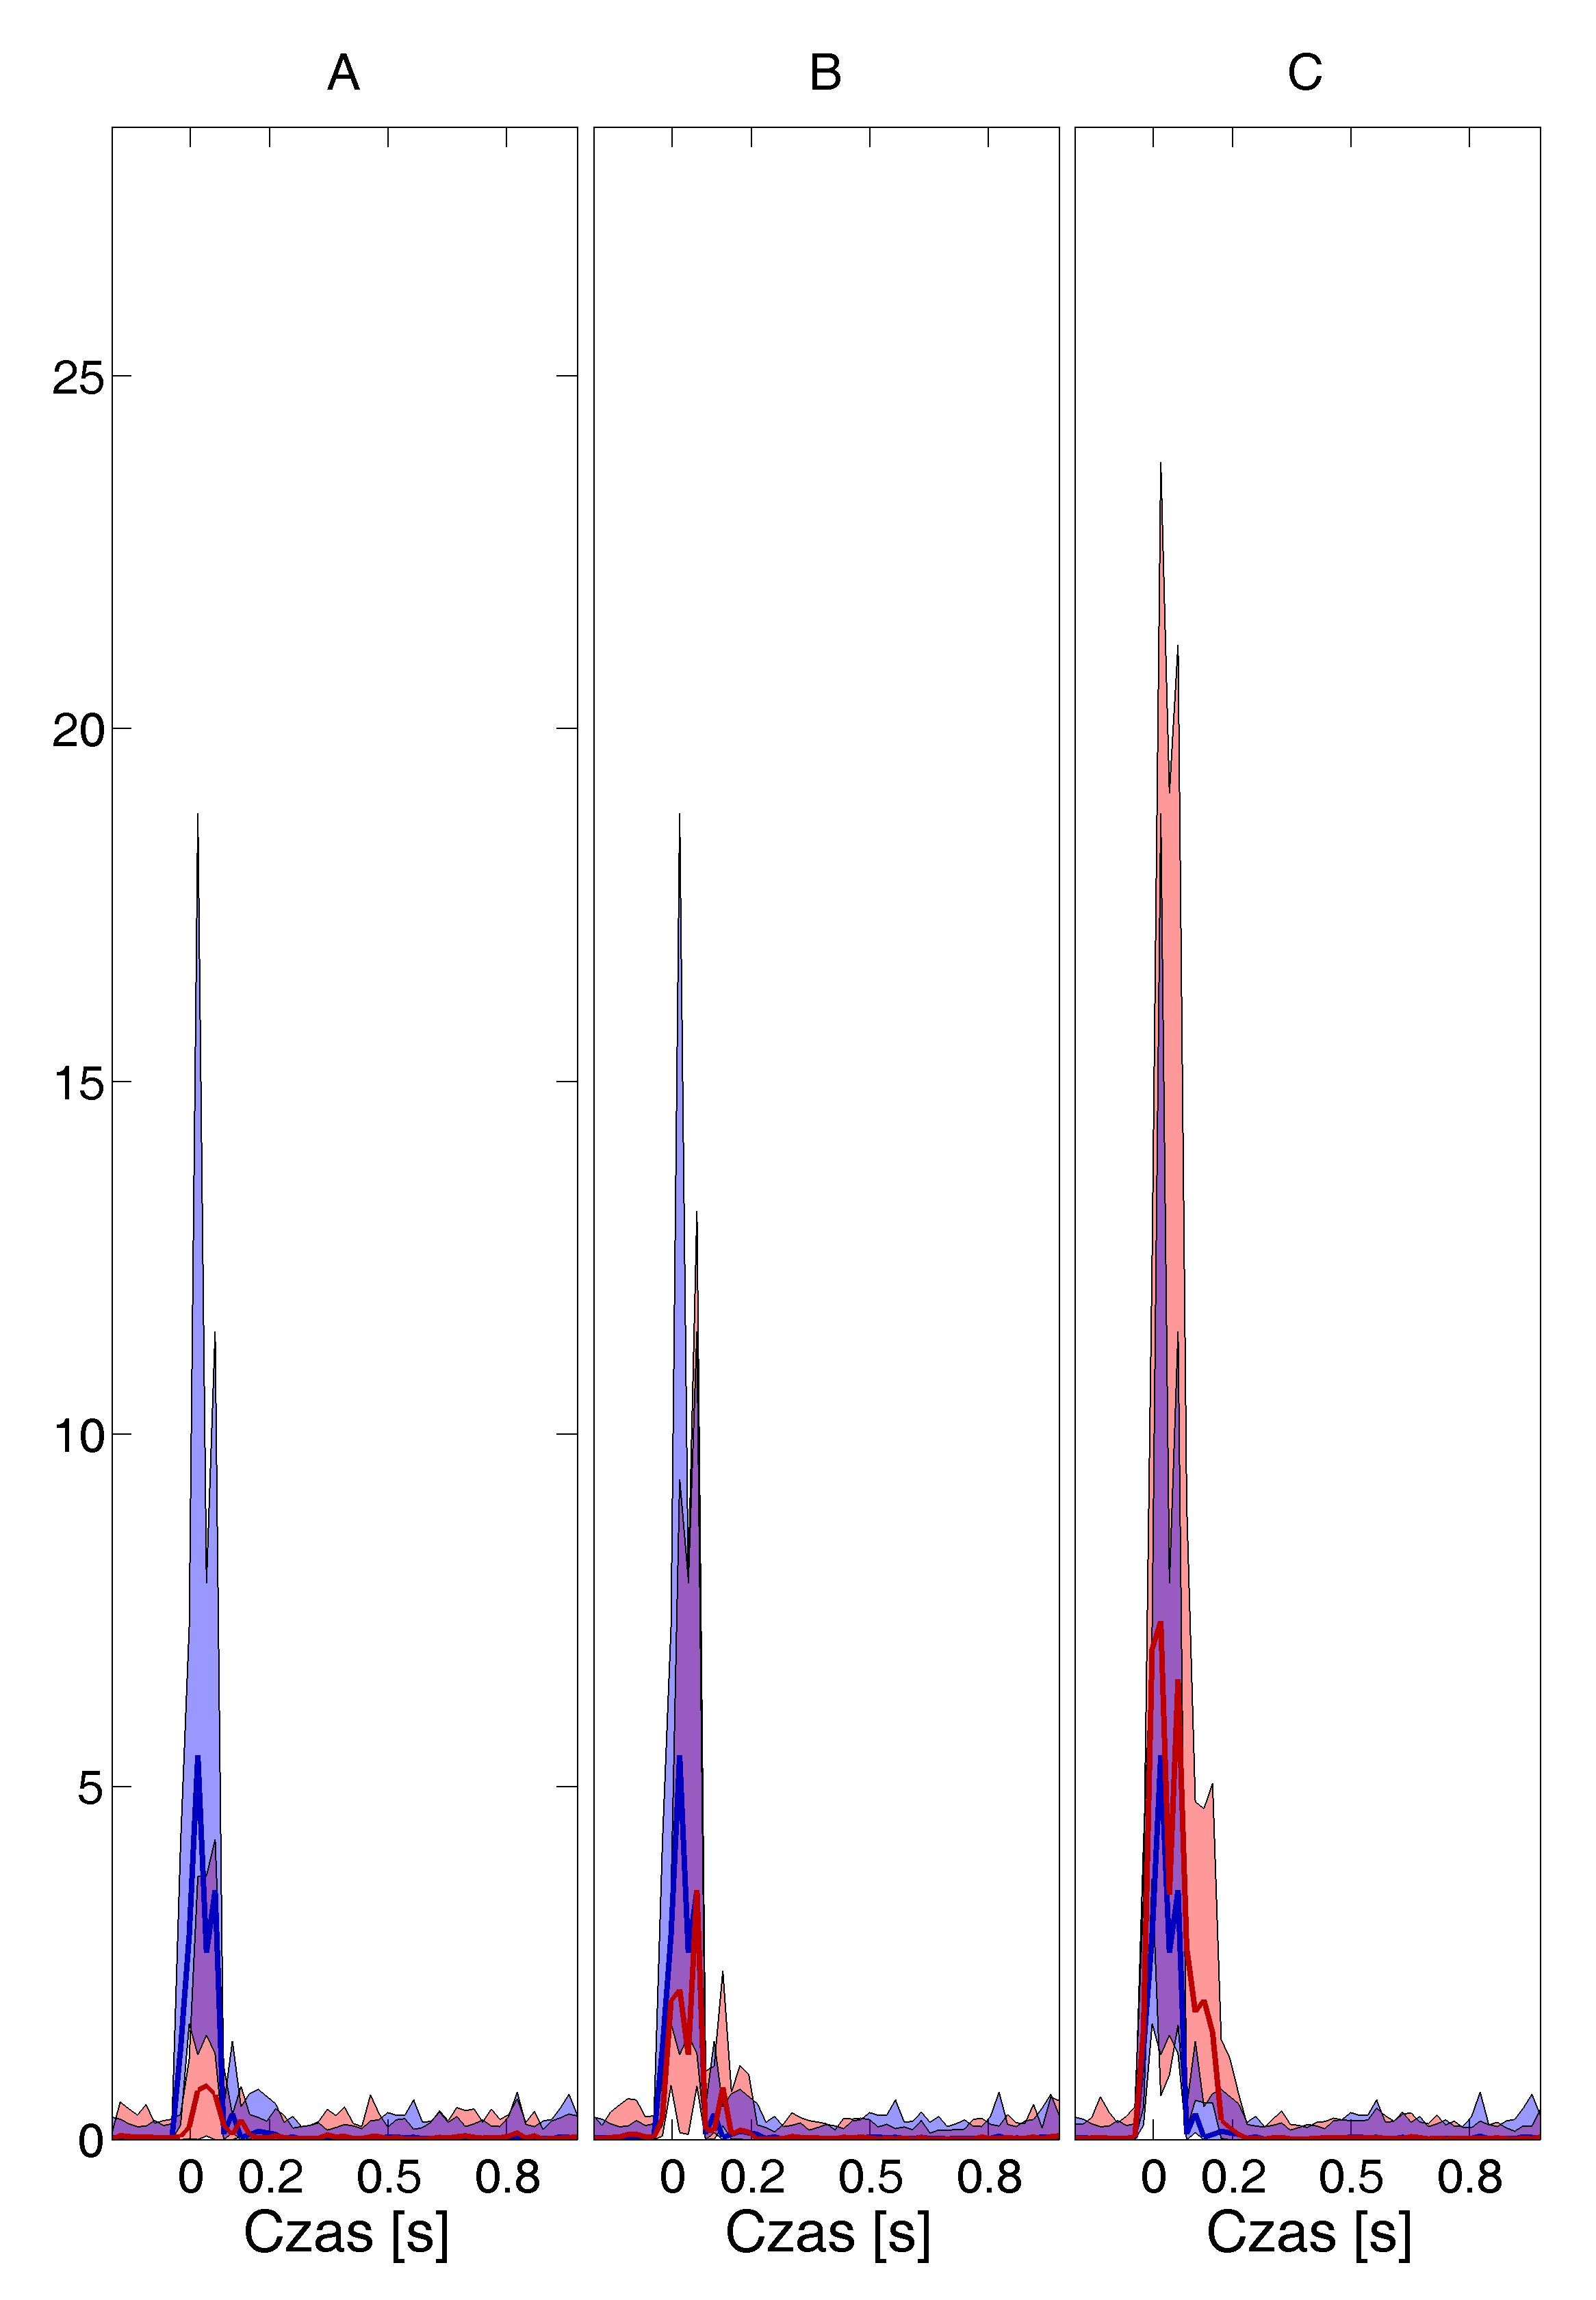
\includegraphics[width=1.\linewidth]{kontrola15_20-40_z_CxC8_do_SC42.png}
			\caption{Bez stymulacji elektrycznej}
			\label{rys:20_40_kon_CxC_SC}
		\end{subfigure}%
		\begin{subfigure}{.5\textwidth}
			\centering
			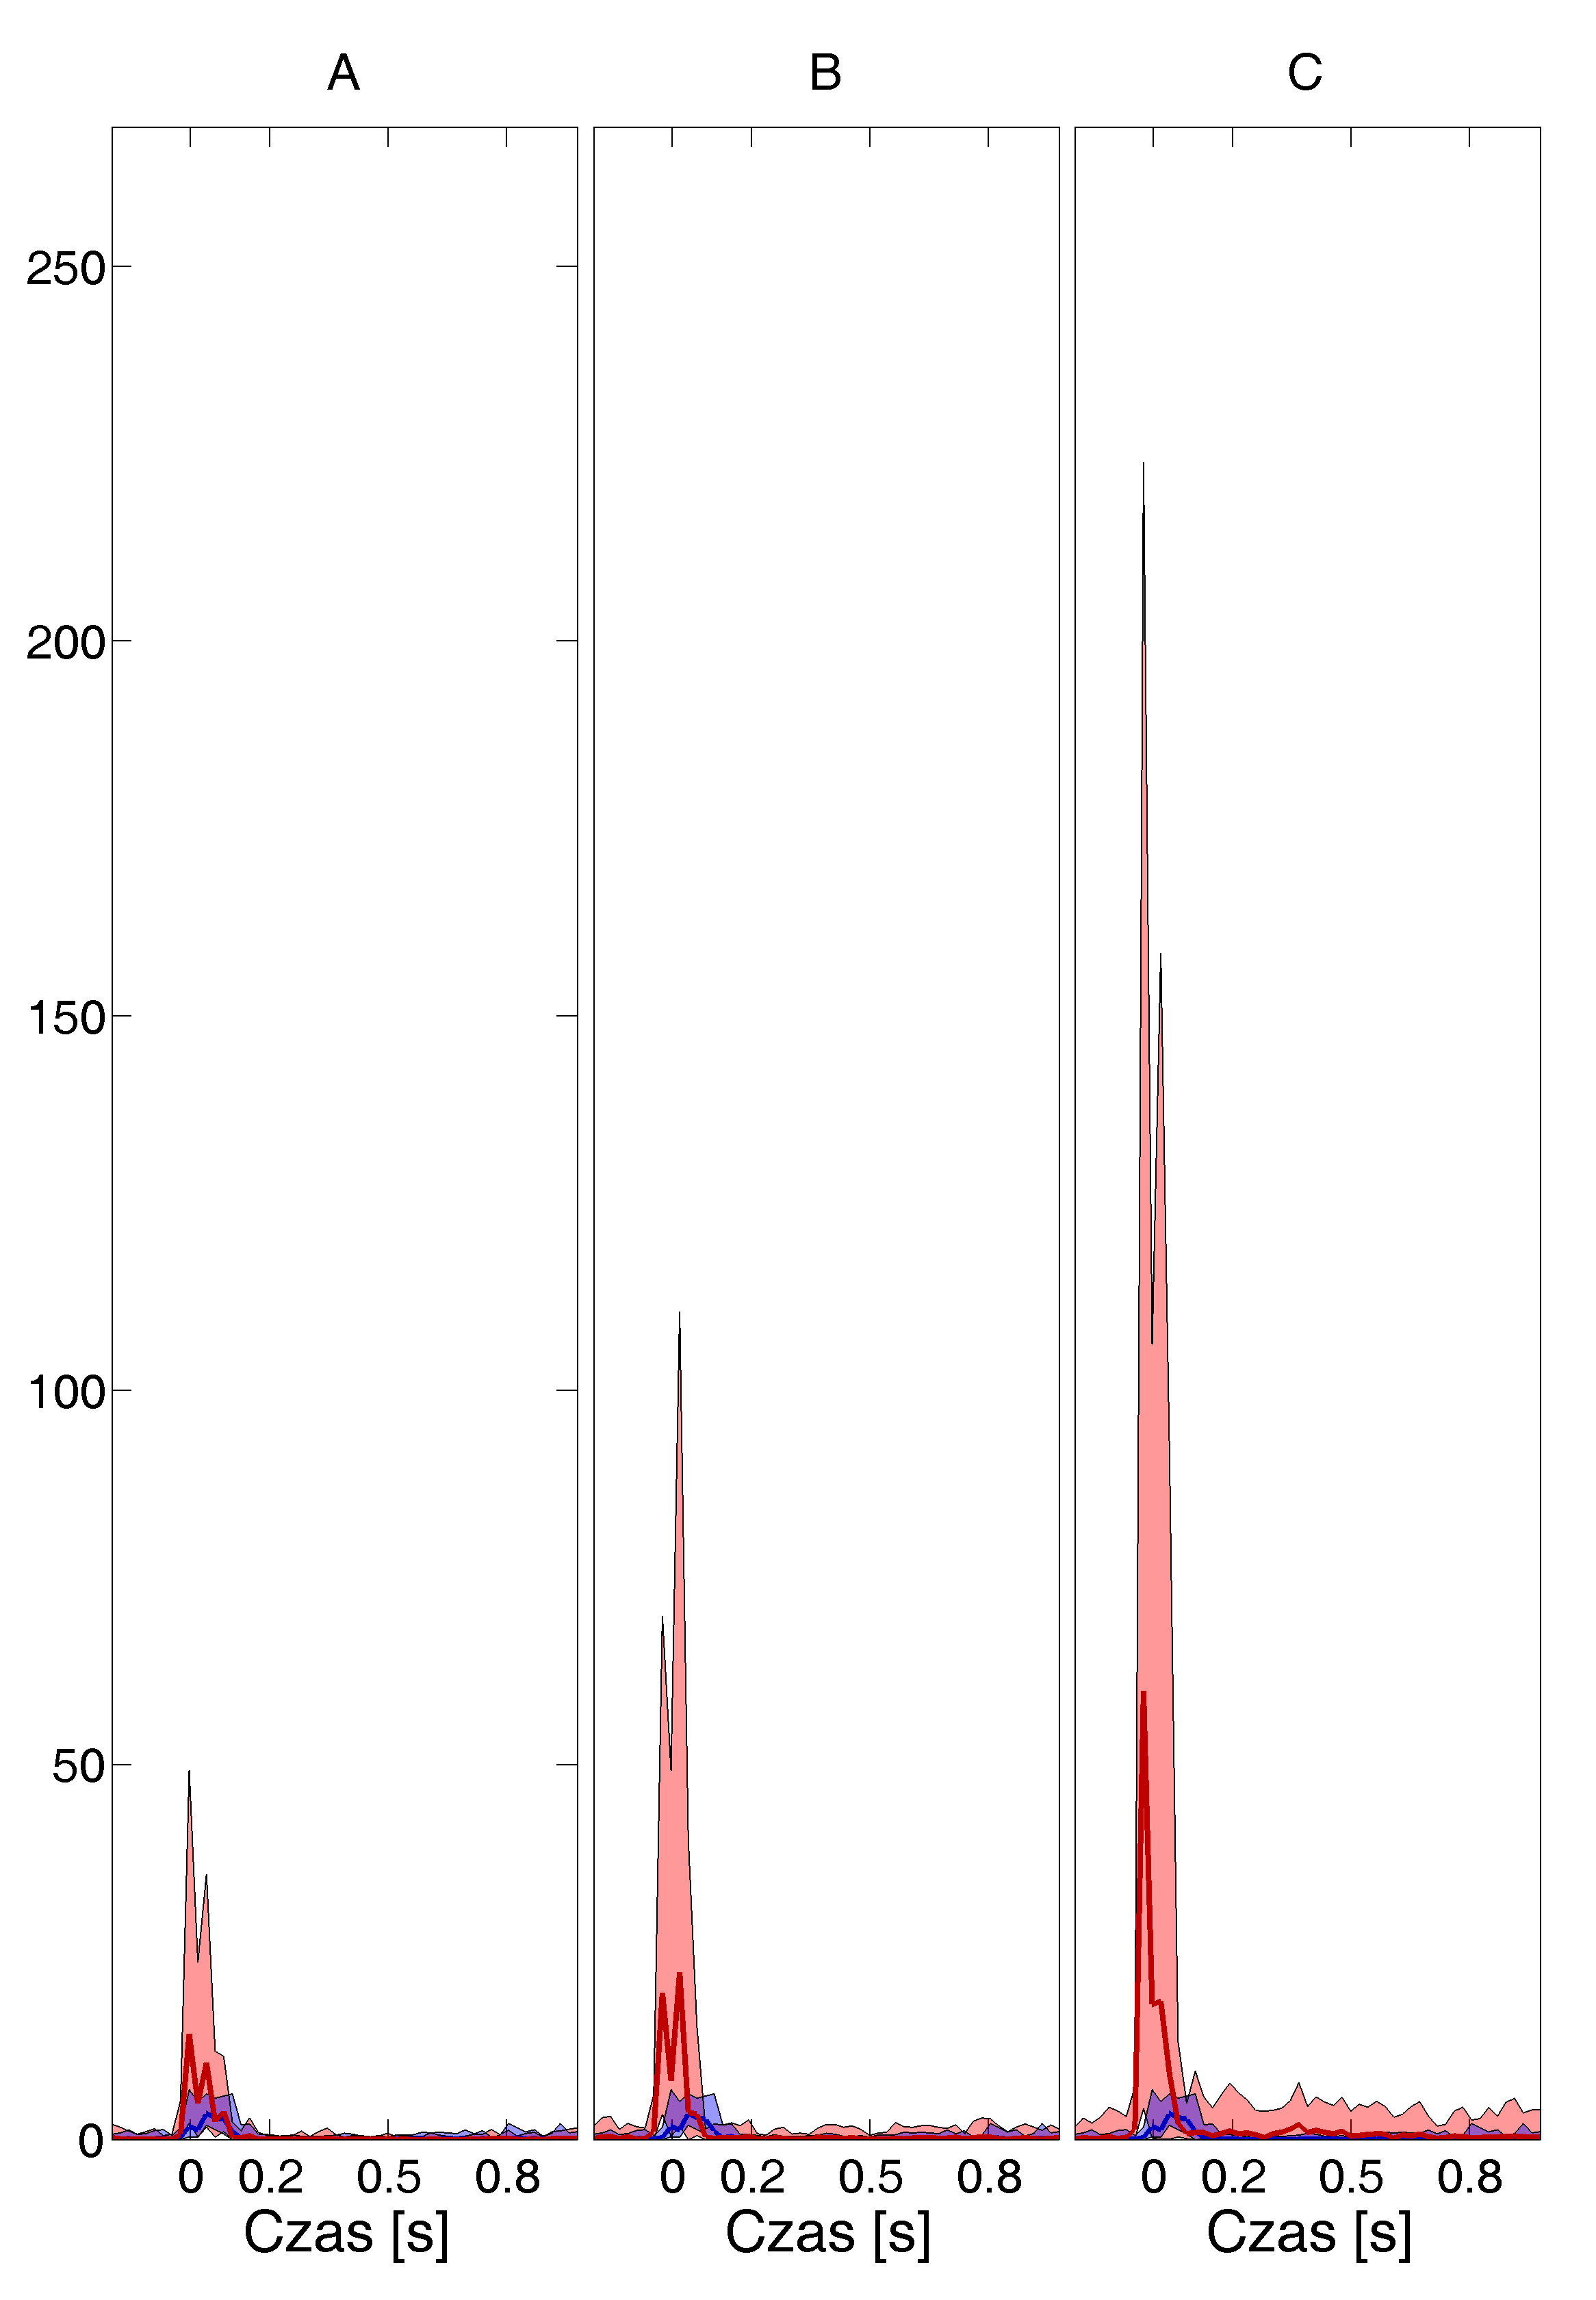
\includegraphics[width=1.\linewidth]{beta3_20-40_z_CxC5_do_SC42.png}
			\caption{Po stymulacji elektrycznej}
			\label{rys:20_40_beta_CxC_SC}
		\end{subfigure}
		\caption{Przedstawienie danych z różnych eksperymentów w paśmie 20-40 Hz.}
		\label{rys:20_40_CxC_SC}
	\end{figure}
	\FloatBarrier
	%\newpage
	\subsection{Połączenia z SC do CxC}
	Do analizy wykorzystano kanały: z zestawu A SC6 i CxC10 oraz z zestawu B: SC2 i CxC8.
	W paśmie 1-10 Hz (Rysunek \ref{rys:1_10_SC_CxC}) dla obu warunków doświadczalnych widoczne są piki w 0,2 s. Dla danych z eksperymentu A (Rysunek \ref{rys:1_10_kon_SC_CxC}) stosunkowo wysoka wartość funkcji NDTF w czasie 0-0,1 s utrzymuje się przez cały czas trwania treningu. Dla danych z eksperymentu B (Rysunek \ref{rys:1_10_beta_SC_CxC}) wysoka wartość funkcji NDTF w czasie 0-0,1 s po każdej godzinie treningu maleje.
	\begin{figure}[h]
		\begin{subfigure}{.5\textwidth}
			\centering
			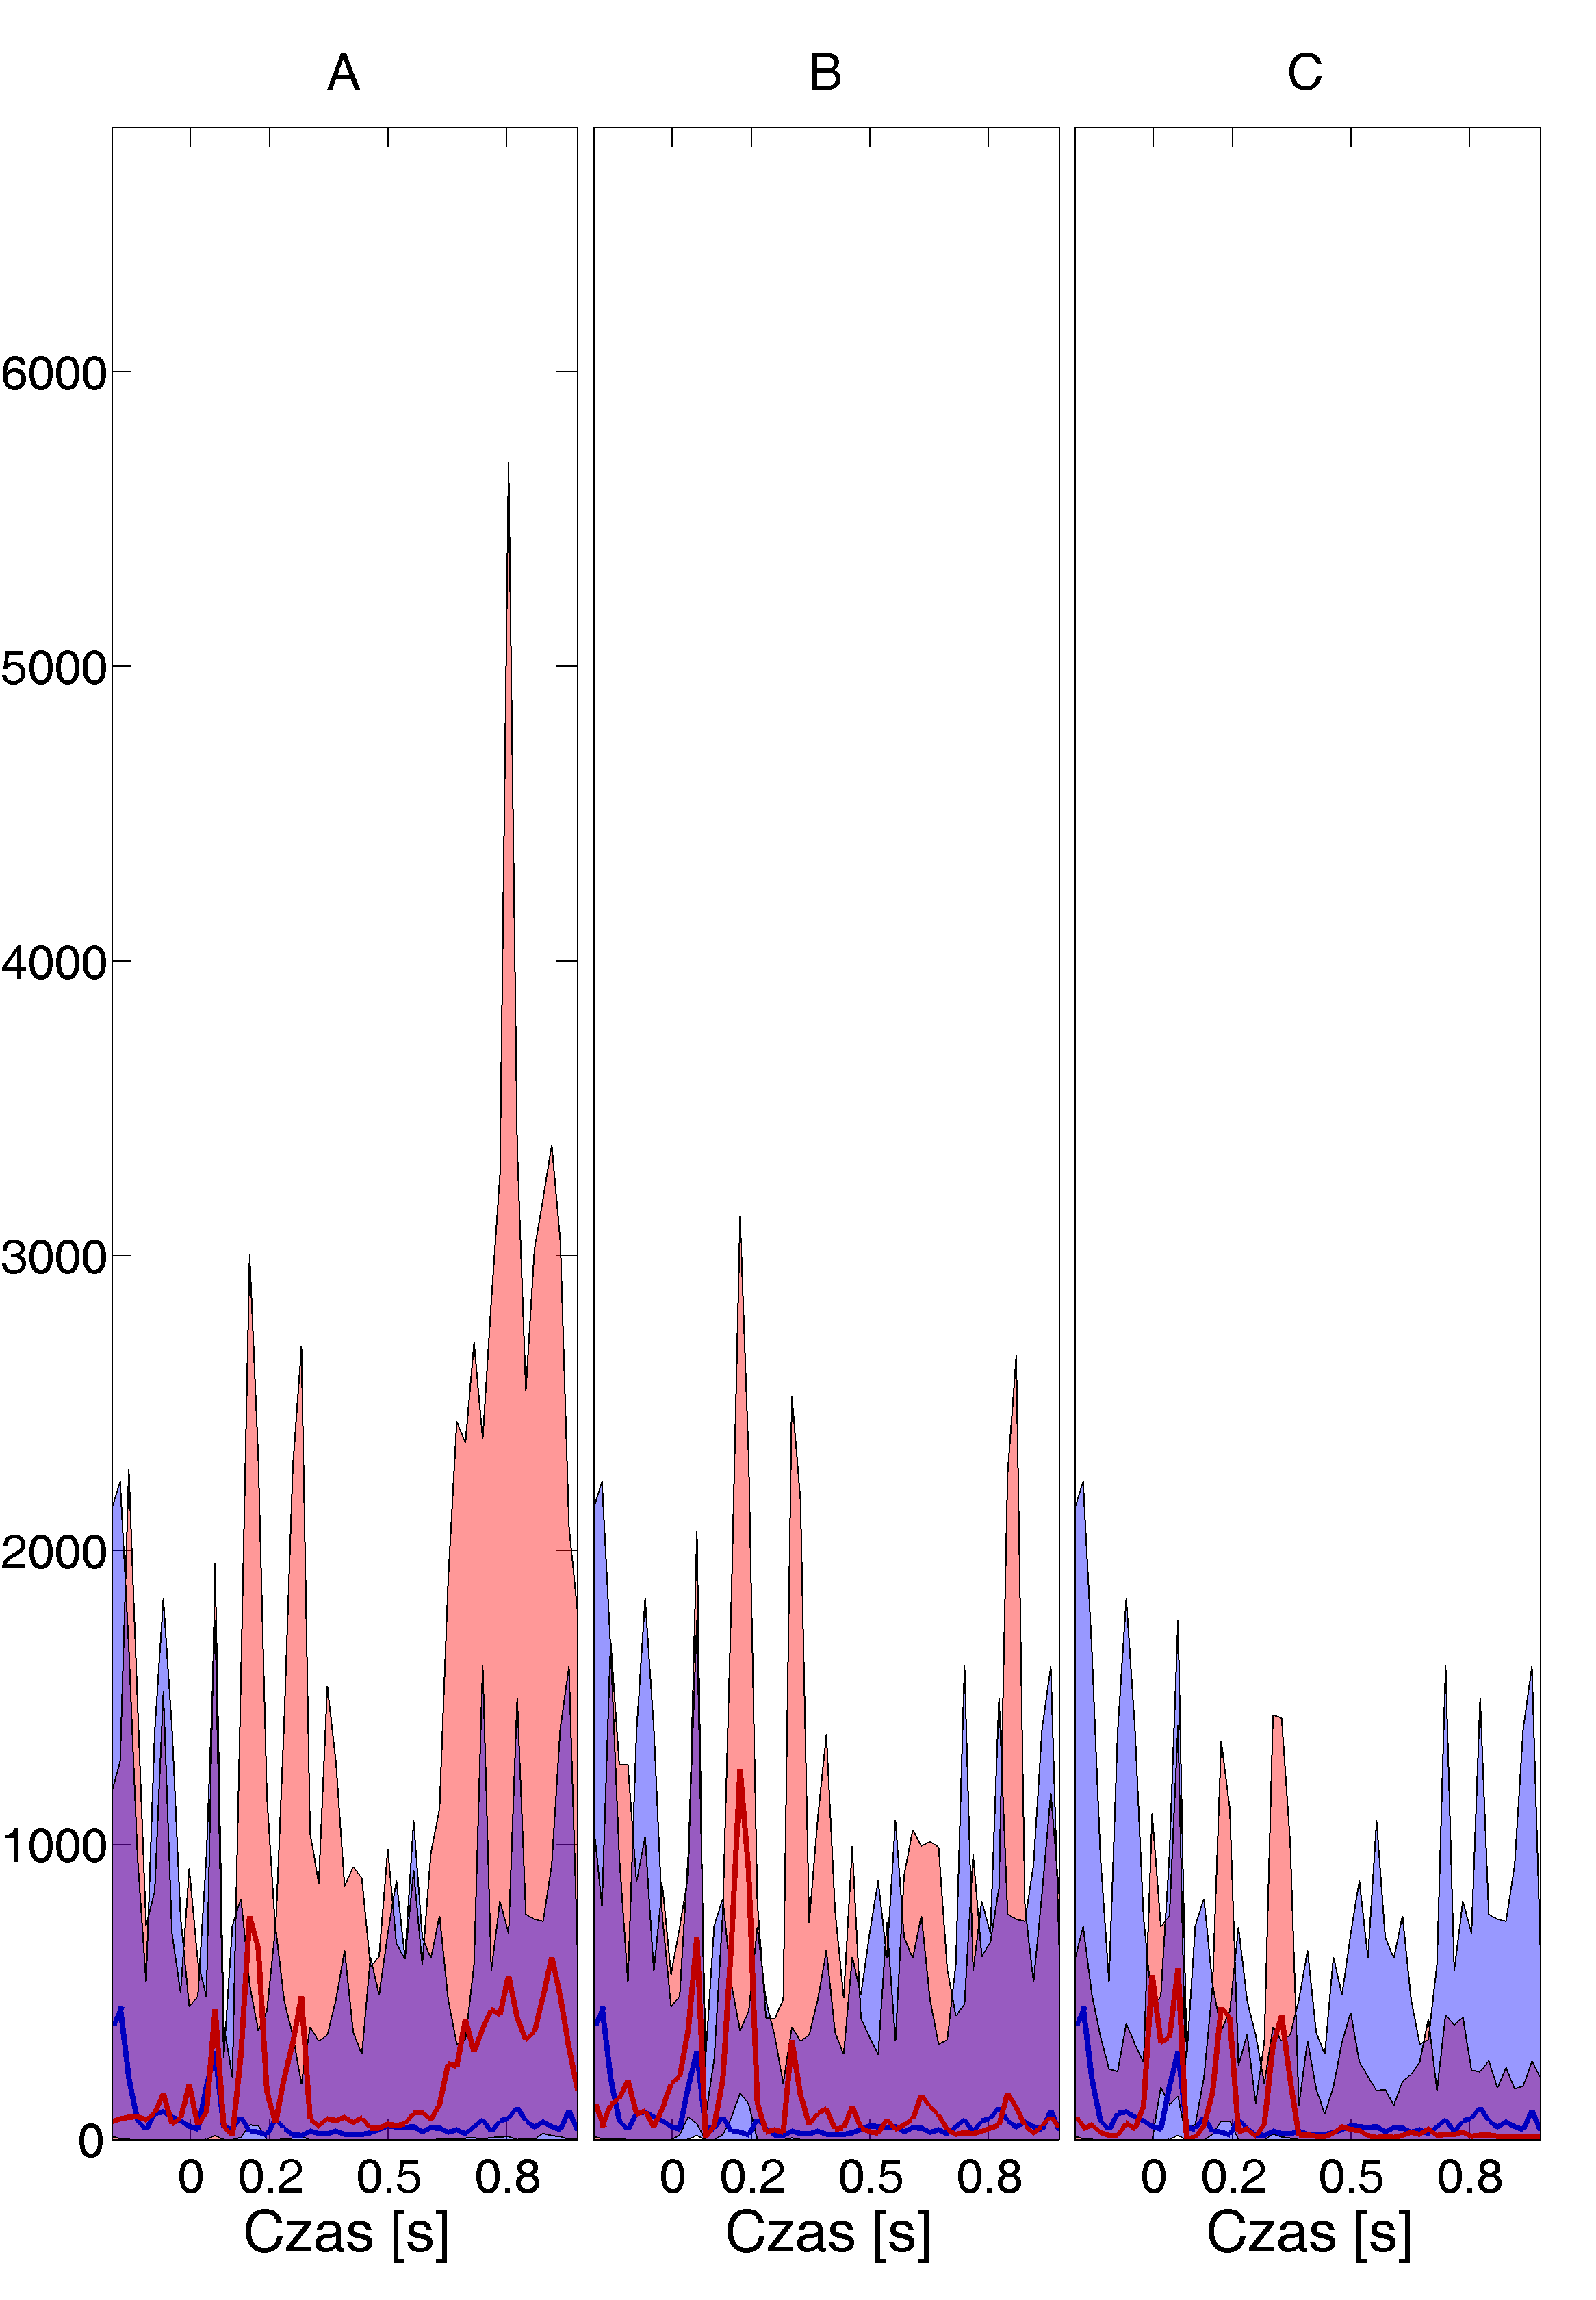
\includegraphics[width=1.\linewidth]{kontrola15_1-10_z_SC6_do_CxC102.png}
			\caption{Bez stymulacji elektrycznej}
			\label{rys:1_10_kon_SC_CxC}
		\end{subfigure}%
		\begin{subfigure}{.5\textwidth}
			\centering
			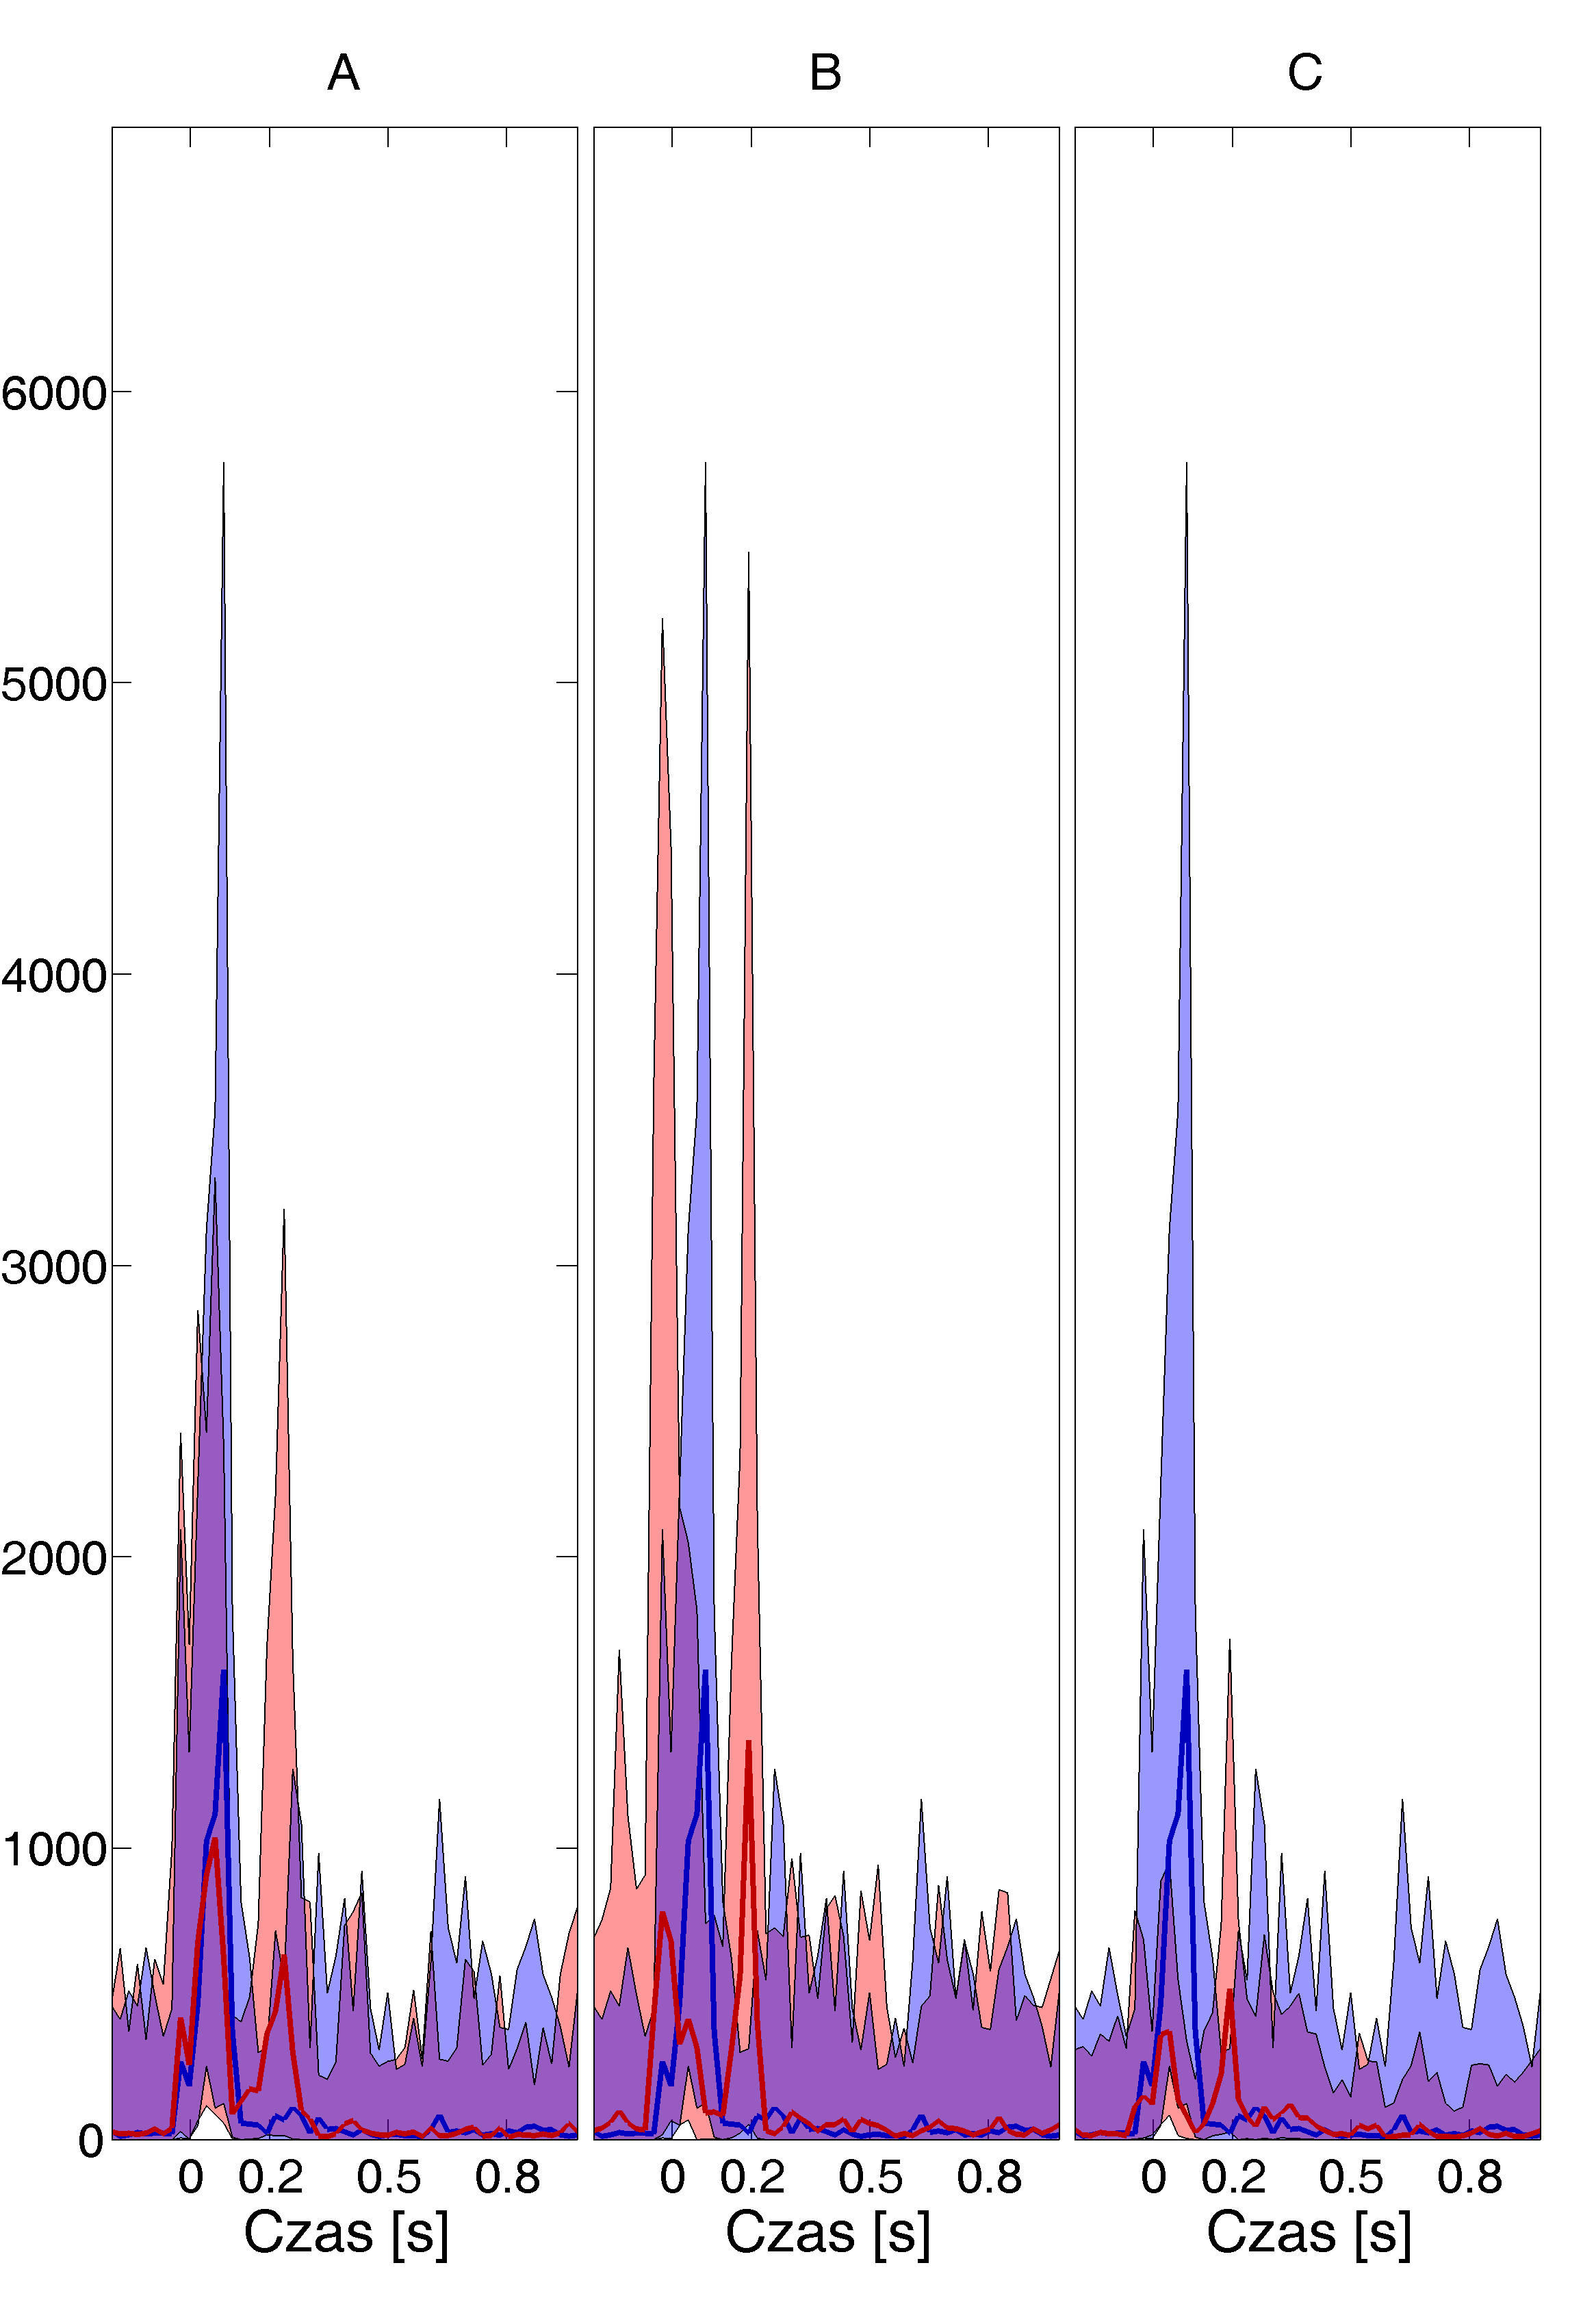
\includegraphics[width=1.\linewidth]{beta3_1-10_z_SC2_do_CxC82.png}
			\caption{Po stymulacji elektrycznej}
			\label{rys:1_10_beta_SC_CxC}
		\end{subfigure}
		\caption{Przedstawienie danych z różnych eksperymentów w paśmie 1-10 Hz.}
		\label{rys:1_10_SC_CxC}
	\end{figure}
	\FloatBarrier
	W paśmie 10-30 Hz dla obu zestawów danych (Rysunek \ref{rys:10_30_SC_CxC}) widoczne są piki w czasie 0-0,1 s i w 0,2 s. Jednakże różnica wartości funkcji NDTF między kolejnymi godzinami treningu a kontrolą jest znacznie większa dla danych z eksperymentu~A (Rysunek \ref{rys:10_30_kon_SC_CxC}) niż dla danych z eksperymentu B (Rysunek \ref{rys:10_30_beta_SC_CxC}).
	\begin{figure}[h]
		\begin{subfigure}{.5\textwidth}
			\centering
			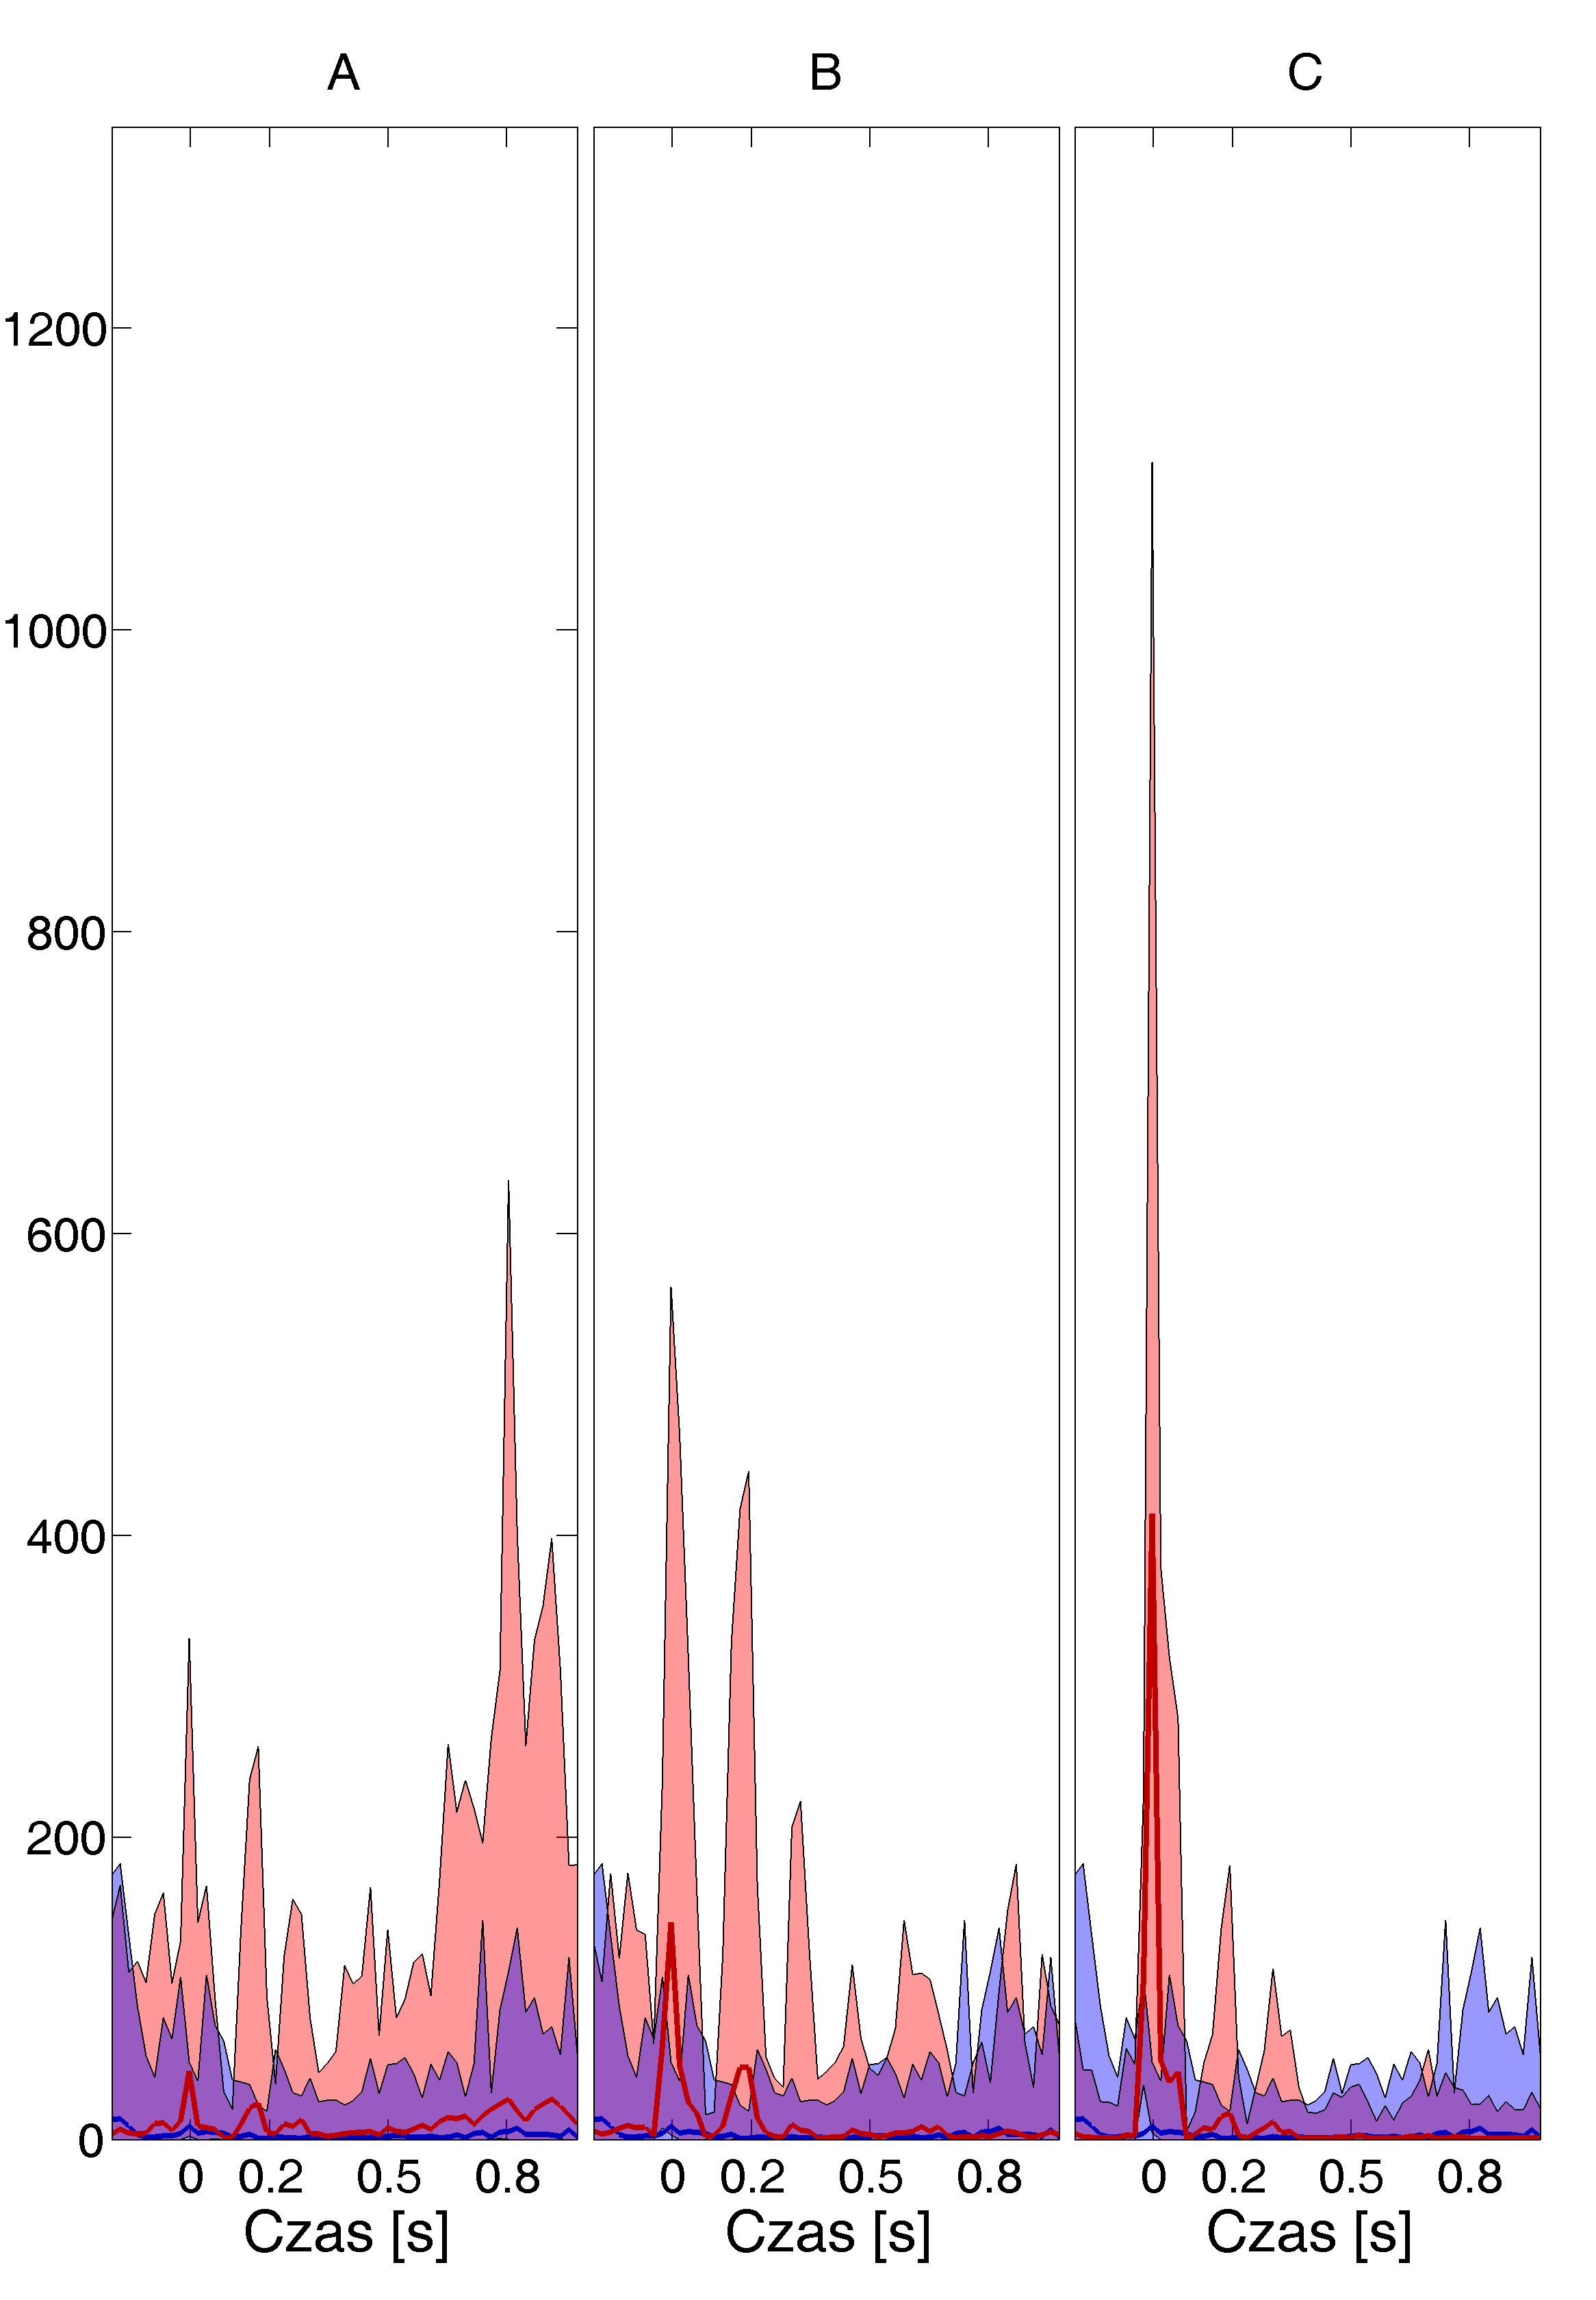
\includegraphics[width=1.\linewidth]{kontrola15_10-30_z_SC6_do_CxC102.png}
			\caption{Bez stymulacji elektrycznej}
			\label{rys:10_30_kon_SC_CxC}
		\end{subfigure}%
		\begin{subfigure}{.5\textwidth}
			\centering
			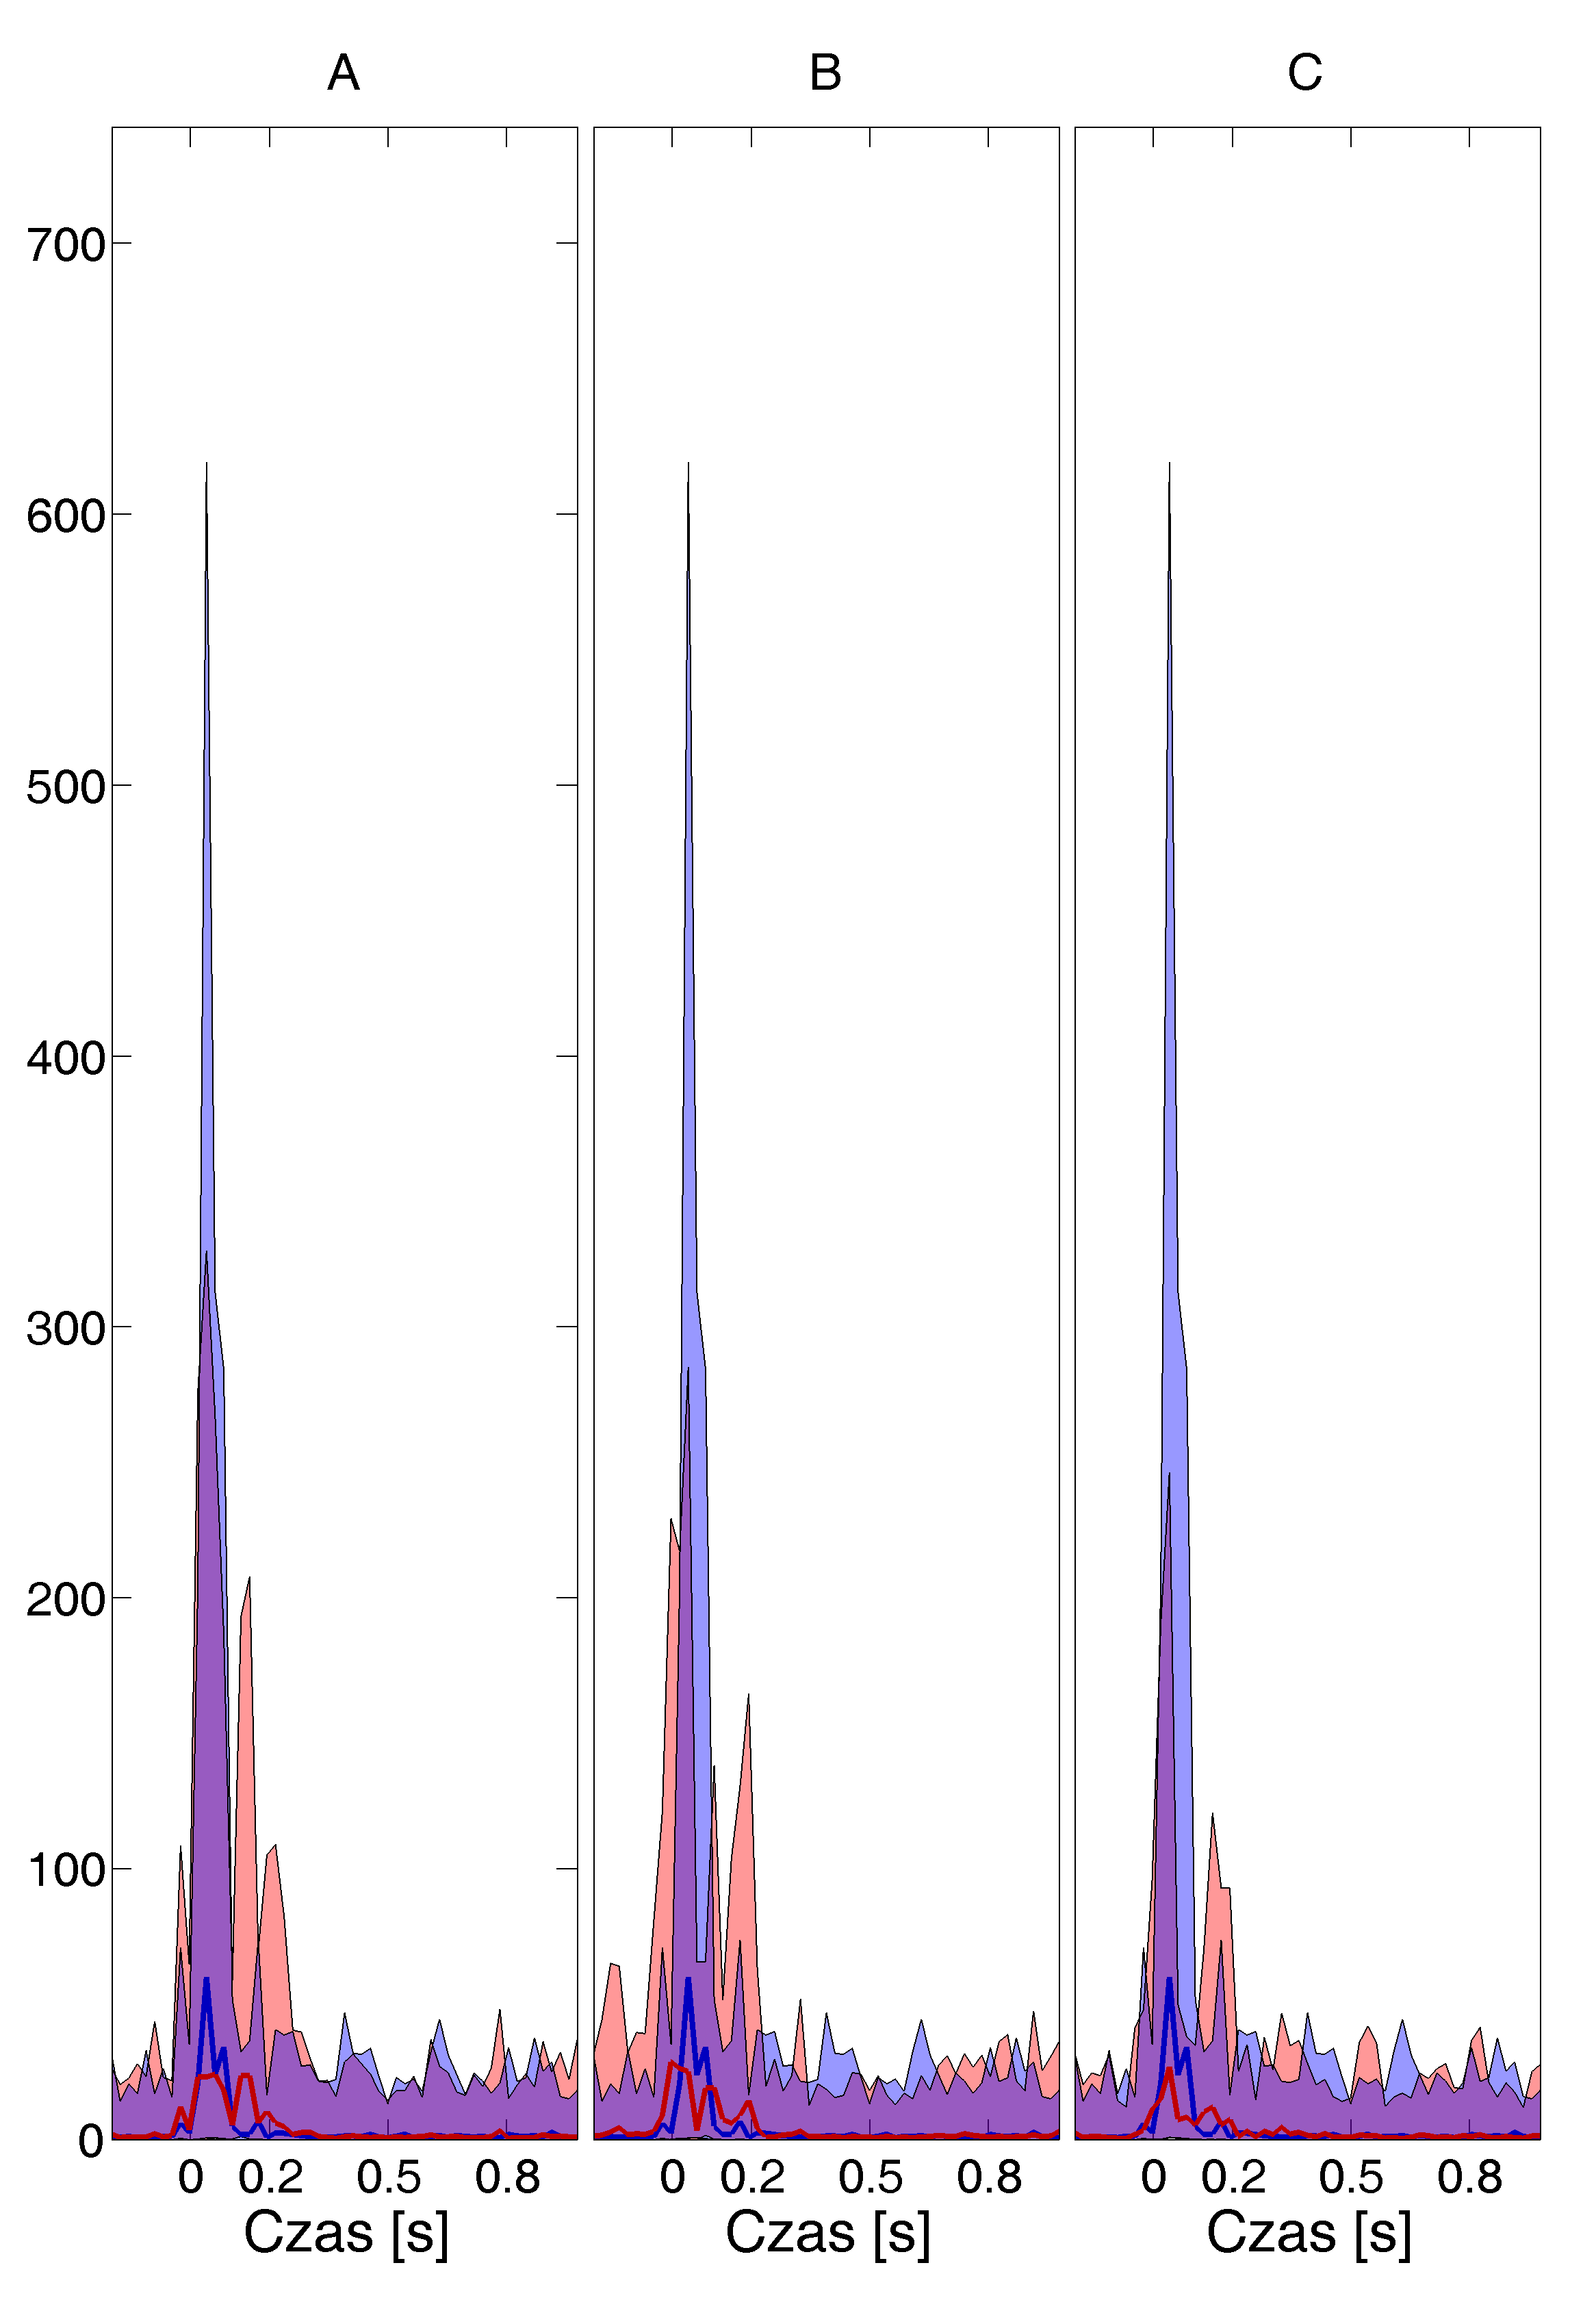
\includegraphics[width=1.\linewidth]{beta3_10-30_z_SC2_do_CxC82.png}
			\caption{Po stymulacji elektrycznej}
			\label{rys:10_30_beta_SC_CxC}
		\end{subfigure}
		\caption{Przedstawienie danych z różnych eksperymentów w paśmie 10-30 Hz.}
		\label{rys:10_30_SC_CxC}
	\end{figure}
	\FloatBarrier
	Na Rysunku \ref{rys:20_40_SC_CxC} przedstawiono wartości funkcji NDTF dla zakresu częsrości 20-40 Hz. Dla danych z eksperymentu A (Rysunek \ref{rys:20_40_kon_SC_CxC}) widoczny jest wysoki pik w czasie 0 s, co jest zapewne efektem zakłócenia wywołanego prezentacją bodźca. Poza tym, dla obu warunków doświadczalnych nie widać różnic między danymi kontrolnymi a każdą kolejną godziną treningu.
	\begin{figure}[h]
		\begin{subfigure}{.5\textwidth}
			\centering
			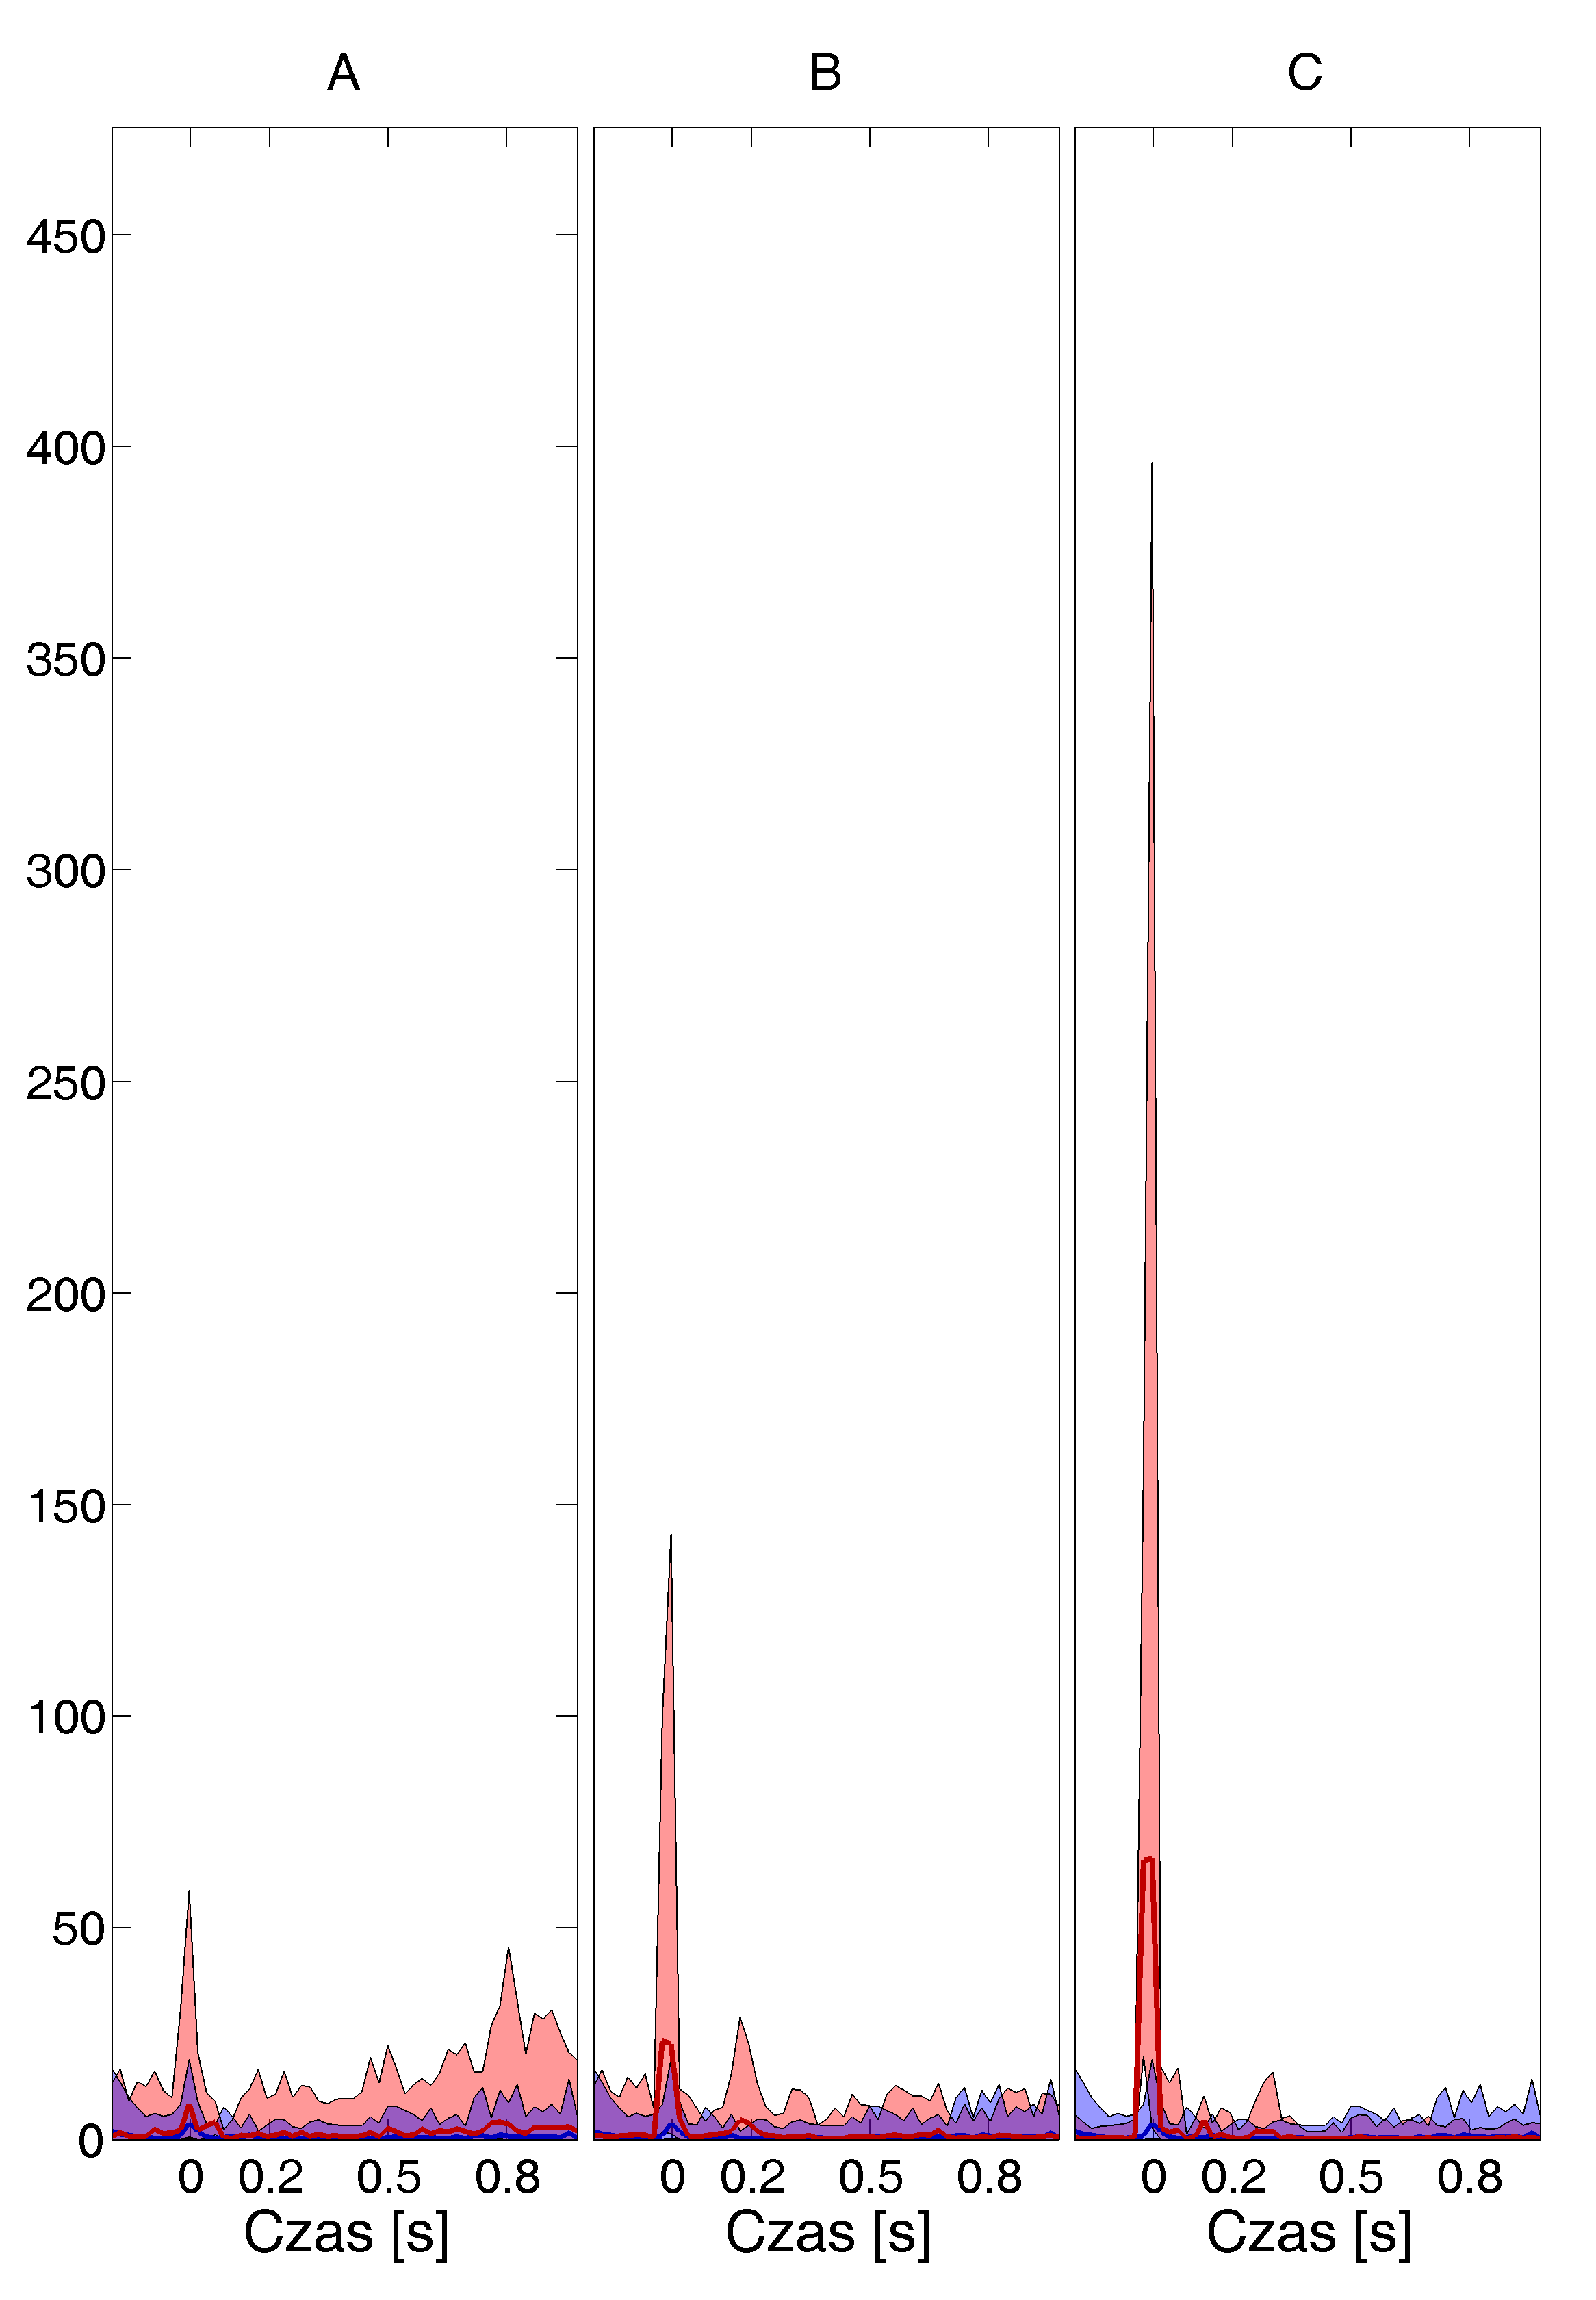
\includegraphics[width=1.\linewidth]{kontrola15_20-40_z_SC6_do_CxC102.png}
			\caption{Bez stymulacji elektrycznej}
			\label{rys:20_40_kon_SC_CxC}
		\end{subfigure}%
		\begin{subfigure}{.5\textwidth}
			\centering
			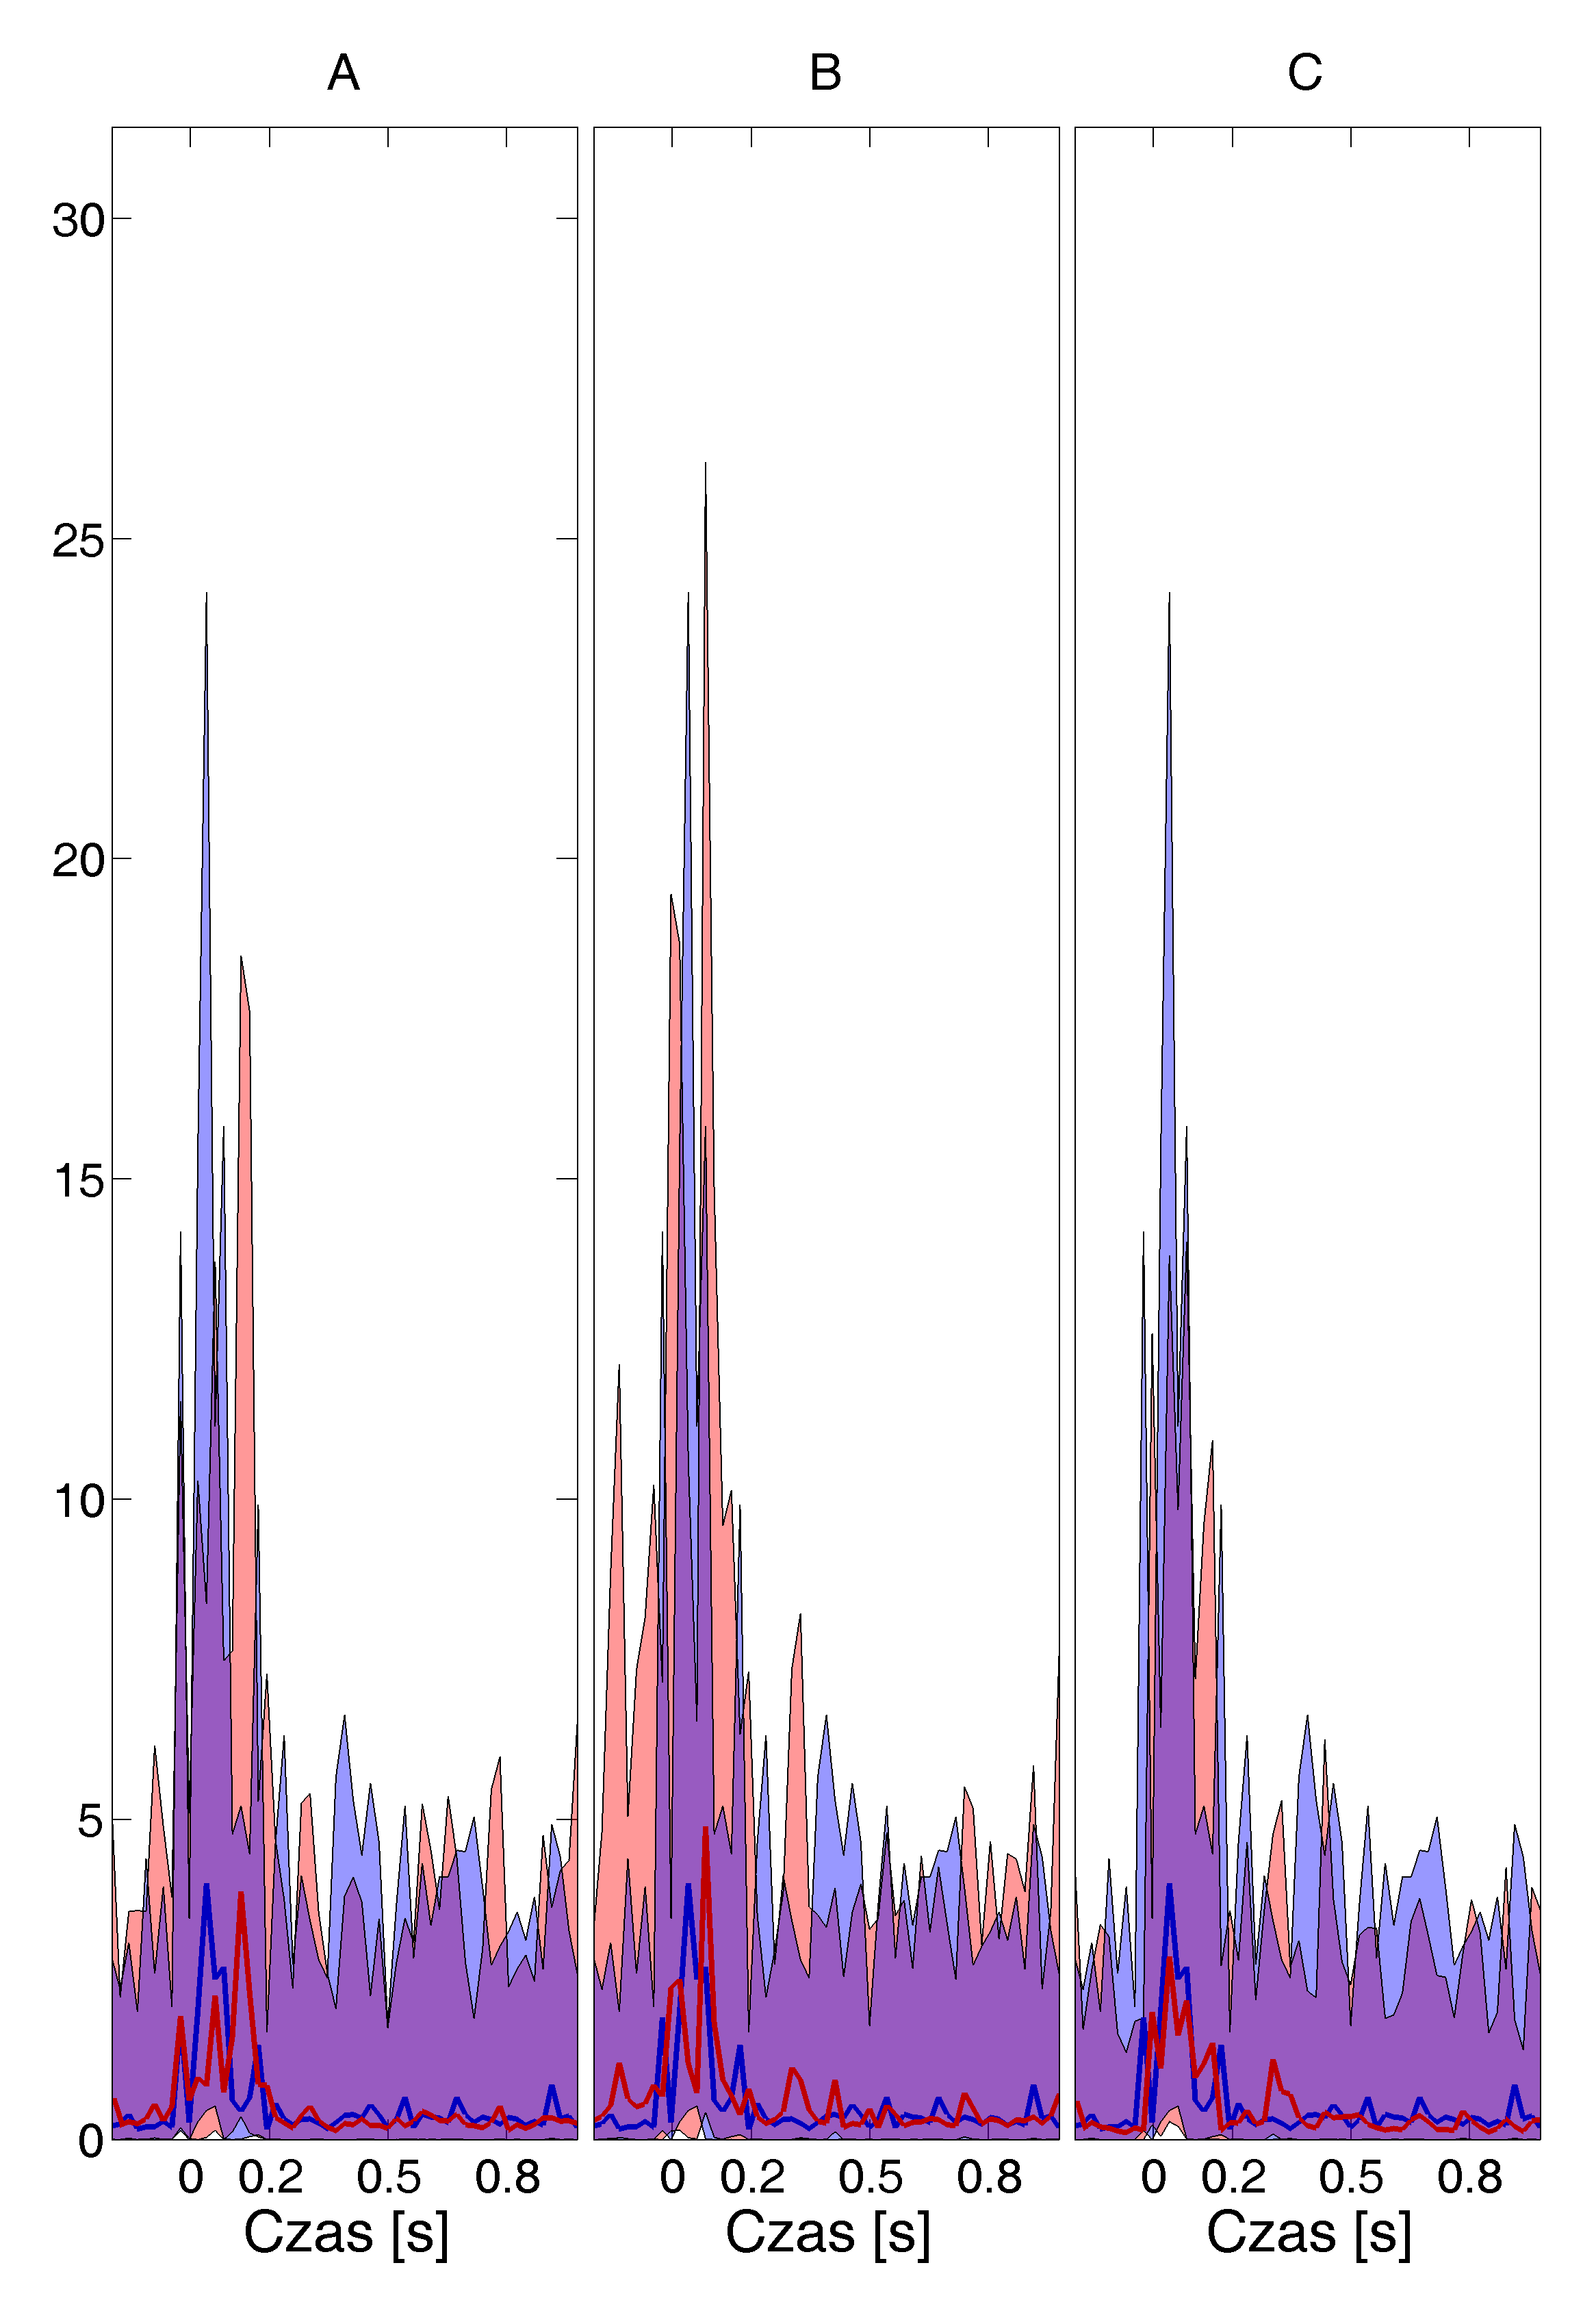
\includegraphics[width=1.\linewidth]{beta3_20-40_z_SC2_do_CxC82.png}
			\caption{Po stymulacji elektrycznej}
			\label{rys:20_40_beta_SC_CxC}
		\end{subfigure}
		\caption{Przedstawienie danych z różnych eksperymentów w paśmie 20-40 Hz.}
		\label{rys:20_40_SC_CxC}
	\end{figure}
	\FloatBarrier
	\subsection{Połączenia z LGN do CxC}
	Dla żadnego zestawu danych, niezależnie od dobieranych zakresów częstości nie udało się zaobserwować połączenia między tymi strukturami.
	\chapter{Dyskusja}
	Przede wszystkim należy podkreślić, że niniejsza praca jest właściwe zaprezentowaniem metod analizy. Wykorzystano jedynie po jednym szczurze z każdego paradygmatu, więc nie ma pewności, że zaprezentowane zależności nie są wynikiem różnorodności osobniczych. Po drugie, występują różnice w budowie mózgów poszczególnych zwierząt, za czym idą także różnice w rozmieszczeniu struktur mózgowych. Dlatego nie można mieć pewności, że wybrane do porównania kontakty były umieszczone na tej samej głębokości. W celu wykonania rzeczywistego porównania należałoby przeanalizować więcej zwierząt z obu warunków doświadczalnych. 

	Analiza statystyczna uśrednionych potencjałów wywołanych powala stwierdzić, że obserwowany wzrost amplitudy wraz z treningiem wzrokowym jest istotny statystycznie. Nie można jednak jednoznacznie rozstrzygnąć, czy stymulacja elektryczna przed przystąpieniem do treningu wzrokowego istotnie tę amplitudę zwiększa. Dla rejestracji z kontralateralnej kory wzrokowej po stymulacji elektrycznej rzeczywiście obserwuje się wzrost już po pierwszej godzinie treningu, co nie występuje po samym treningu wzrokowym (tylko w 2 z 4 kanałów wykazano istotny wzrost amplitudy po pierwszej godzinie treningu). W przypadku rejestracji z ipsilateralnej kory wzrokowej testy statystyczne wykazały, że stymulacja elektryczna przed treningiem wzrokowym nie spowodowała znaczącego wzrostu amplitudy. Dopiero po trzeciej godzinie treningu wzrost amplitudy był istotny statystycznie. Jednakże ze względu na nietypowy kształt potencjału, można podejrzewać, że elektroda nie została dobrze umieszczona i rejestrowany sygnał nie musi być odpowiedzią ipsilateralnej kory wzrokowej. W przypadku wzgórka czworaczego górnego wzrost amplitudy jest istotny po każdej godzinie treningu dla obu warunków doświadczalnych.
	
	Nieznormalizowana funkcja przejścia pozwala na określenie kierunku oddziaływania między danymi źródłowymi w częstości i czasie. Jak nadmieniono we wstępie, informacja wzrokowa jest przetwarzana dwiema drogami. Jedna z nich prowadzi przez jądro kolankowate boczne do kory wzrokowej, a druga przez wzgórek czworaczy górny i kompleks tylno-boczny poduszki do kory wzrokowej. Kora wzrokowa wysyła również informację zwrotną zarówno do LGNu \citep{viola2}, jak i do wzgórka \citep{viola}. Z tego względu analizowano połączenia między wymienionymi strukturami mózgowymi w obu kierunkach.
	
	Dla pary CxC-LGN udało się zaobserwować wzrost funkcji NDTF zaraz po zaprezentowaniu bodźca wzrokowego, co jest szczególnie widoczne dla zestawu danych po stymulacji elektrycznej. Niestety nie udało się wykryć połączenia między jądrem kolankowatym bocznym a kontralateralną korą wzrokową. Wytłumaczeniem może być fakt, że ponieważ LGN jest niewielką strukturą położoną głęboko pod warstwą korową, dostęp do niej jest utrudniony i być może nie trafiono elektrodą dokładnie w tę strukturę.
	
	Kolejnymi analizowanymi połączeniami, były te między korą wzrokową a wzgórkiem czworaczym górnym. Dla pary CxC-SC w obu warunkach doświadczalnych zaobserwowano znaczący wzrost funkcji NDTF względem danych kontrolnych zaraz po zaprezentowaniu bodźca wzrokowego. Dla połączeń SC-CxC wysoka wartość funkcji NDTF względem danych kontrolnych utrzymywała się na stałym poziomie dla zestawu danych bez stymulacji elektrycznej. Natomiast dla danych po stymulacji elektrycznej ta wartość wraz z długością treningu spadała.
	
	Jest możliwe, że brak istotnych różnic w amplitudzie potencjału wywołanego jest spowodowany zbyt krótkim czasem stymulacji elektrycznej. W innych tego rodzaju badaniach stosowano znacząco dłuższy czas stymulacji np. 30 min \citep{lazzaro}.
	
	Przy analizie porównawczej funkcji NDTF należałoby wykorzystać więcej szczurów, by przekonać się, czy wykryte zależności powtarzają się dla większej grupy badanych zwierząt.

	\bibliography{bibliography}
	
\end{document}


%%% Local Variables:
%%% mode: latex
%%% TeX-master: t
%%% coding: latin-2
%%% End:
